%\subsection{Phương trình mặt phẳng}
\begin{name}
	{\tenchude}
	{TOÁN 12 - PHƯƠNG TRÌNH MẶT PHẲNG}
	{LỚP TOÁN THẦY PHÁT}
	{Thời gian: 90 phút - Không kể thời gian phát đề}
\end{name}
\Opensolutionfile{ans}[ans/ans-0-B15]
\caulc
\begin{ex}%[2H5N1-2]
	Trong không gian $Oxyz$, cho mặt phẳng $(P)\colon x-2 y+3 z+1=0$. Hỏi véc-tơ nào dưới đây là một véc-tơ pháp tuyến của mặt phẳng $(P)$?
	\choice
	{\True $(1;-2; 3)$}
	{$(1; 2; 3)$}
	{$(-2; 3; 1)$}
	{$(2;-2; 4)$}
	\loigiai{
		Véc-tơ $(1;-2; 3)$ là một véc-tơ pháp tuyến của mặt phẳng $(P)$.
	}
\end{ex}
\begin{ex}%[2H5N1-4]
	Trong không gian $Oxyz$, cho hai mặt phẳng $(P)\colon x-y-2z+1=0$ và $(Q)\colon mx+(3-2m)y+nz+1=0$. Khi hai mặt phẳng $(P)$ và $(Q)$ song song với nhau thì giá trị của biểu thức $T=m+n$ bằng
	\choice
	{$1$}
	{$0$}
	{\True $-3$}
	{$5$}
	\loigiai{
		Hai mặt phẳng $(P)$ và $(Q)$ song song với nhau khi và chỉ khi \[\dfrac{m}{1}=\dfrac{3-2m}{-1}=\dfrac{n}{-2}\neq \dfrac{1}{1}\Leftrightarrow \heva{&m=3\\&n=-6.}\]
		Vậy $T=m+n=3-6=-3$.
	}
\end{ex}

\begin{ex}%[2H5H1-3]
	Trong không gian với hệ trục tọa độ $Oxyz$, cho mặt phẳng $(P)\colon 2x-y-2z-1=0$. Mặt phẳng $(Q)$ đi qua gốc tọa độ $O$ và song song với $(P)$ là
	\choice
	{$2x+y-2z=0$}
	{\True $2x-y-2z=0$}
	{$2x-y-2z+1=0$}
	{$2x+2y-z=0$}
	\loigiai{
		Mặt phẳng $(Q)$ song song với $(P)$ nên mặt phẳng $(Q)$ có dạng $2x-y-2z+d=0$ ($ d\neq -1 $).\\
		Mặt phẳng $(Q)$ đi qua gốc $O$ nên $ d=0 $ (thỏa mãn).\\
		Vậy $(P)\colon 2x-y-2z=0$. 
	}
\end{ex}


\begin{ex}%[2H5H1-3]
	Trong không gian $Oxyz$, mặt phẳng $(\alpha)$ đi qua điểm $A(1;2;-3)$ và nhận véc-tơ $\overrightarrow{n}=(2;-1;3)$ làm véc-tơ pháp tuyến có phương trình là
	\choice
	{$x+2y-3z+9=0$}
	{$x+2y-3z-9=0$}
	{\True $2x-y+3z+9=0$}
	{$2x-y+3z-9=0$}
	\loigiai{
		Mặt phẳng $(\alpha)$ đi qua điểm $A(1;2;-3)$ và nhận véc-tơ $\overrightarrow{n}=(2;-1;3)$ làm véc-tơ pháp tuyến có phương trình
		$$2(x-1)-(y-2)+3(z+3)=0 \Leftrightarrow 2x-y+3z+9=0.$$
	}
\end{ex}

\begin{ex}%[2H5N1-1]
	Trong không gian $Oxyz$, điểm $M(1;-3;2)$ thuộc mặt phẳng có phương trình nào sau đây?
	\choice 
	{\True$2x+y-z+3=0$}
	{$3x-y+z-2=0$}
	{$2x+y-z+4=0$}
	{$x-2y-z+1=0$}
	\loigiai{ Thay toạ độ điểm $M(1;-3;2)$ lần lượt vào các mặt phẳng ta được
		\begin{itemize}
			\item $3\cdot 1-1\cdot (-3)+1\cdot 2-2\neq 0$. Do đó $M$ không thuộc mặt phẳng $2x+y-z+3=0$.
			\item $2\cdot 1+1\cdot (-3)-1\cdot 2+4\neq 0$. Do đó $M$ không thuộc mặt phẳng $2x+y-z+4=0$.
			\item $1\cdot 1-2\cdot (-3)-1\cdot 2+1\neq 0$. Do đó $M$ không thuộc mặt phẳng $x-2y-z+1=0$.
			\item $2\cdot 1+1\cdot (-3)-1\cdot 2+3=0$. Do đó $M$ thuộc mặt phẳng $2x+y-z+3=0$.
		\end{itemize}
	}
\end{ex}
\begin{ex}%[2H5H1-3]
	Trong không gian $Oxyz$, cho hai điểm $A(-1;2;0)$, $B(1;1;3)$ và mặt phẳng $(P)\colon x-2y+3z-5=0$. Phương trình của mặt phẳng đi qua hai điểm $A$, $B$ đồng thời vuông góc với $(P)$ là
	\choice
	{$x+2y+z-3=0$}
	{$2x+y-z=0$}
	{\True $x-y-z+3=0$}
	{$x+y-z-1=0$}
	\loigiai
	{
		Ta có $\overrightarrow{AB}=(2;-1;3)$ và véc-tơ pháp tuyến của mặt phẳng $(P)$ là $\overrightarrow{n}_P=(1;-2;3)$.\\
		Gọi $(Q)$ là mặt phẳng đi qua $A$, $B$ và vuông góc $(P)$.\\
		Khi đó véc-tơ pháp tuyến của mặt phẳng $(Q)$ là $$\overrightarrow{n}_Q=\left[\overrightarrow{AB}, \overrightarrow{n}_P\right]=(3;-3;-3)=3(1;-1;-1).$$
		Vậy phương trình mặt phẳng $(Q)$ đi qua $A(-1;2;0)$ và có véc-tơ pháp tuyến $\overrightarrow{n}_Q=(1;-1;-1)$ có phương trình
		$$(Q)\colon x-y-z+3=0.$$
	}
\end{ex}


\begin{ex}%[2H5N1-1]
	Trong không gian $Oxyz$, mặt phẳng $(P)\colon x+2y-2z+1=0$ đi qua điểm nào dưới đây?
	\choice
	{\True $M(1;2;3)$}
	{$N(1;2;-2)$}
	{$P(-1;2;-3)$}
	{$Q(2;-2;1)$}
	\loigiai{
		Thay tọa độ các điểm $M$, $N$, $P$, $Q$ vào phương trình mặt phẳng $(P)$ ta thấy chỉ có điểm $M$ có tọa độ thỏa mãn.\\
		Vậy		mặt phẳng $(P)\colon x+2y-2z+1=0$ đi qua điểm $M(1;2;3)$.
	}
\end{ex}	

\begin{ex}%[2H5H1-3]
	Trong không gian $Oxyz$, cho hai điểm $A(-1;0;2)$, $B(3;2;0)$. Phương trình mặt phẳng trung trực của $AB$ là
	\choice
	{$x+y+z+2=0$}
	{$2 x+y-z+2=0$}
	{$x+y+z-2=0$}
	{\True $2x+y-z-2=0$}
	\loigiai{
		Ta có $\overrightarrow{AB}=(4;2;-2)$.\\
		Gọi $(P)$ là mặt phẳng trung trực của $AB$. Ta có phương trình $(P)$ đi qua trung điểm $I(1;1;1)$ của $AB$ và nhận $\overrightarrow{n}=(2;1;-1) $ làm một véc-tơ pháp tuyến là
		\[ 2(x-1)+(y-1)-(z-1)=0\Leftrightarrow 2x+y-z-2=0.\]
	}
\end{ex}
\begin{ex}%[2H5H1-3]
	Trong không gian với hệ trục tọa độ $Oxyz$, cho điểm $M(1;2;3)$. Gọi $A$, $B$, $C$ lần lượt là hình chiếu vuông góc của điểm $M$ lên các trục $Ox$, $Oy$, $Oz$. Phương trình mặt phẳng $(ABC)$ là
	\choice
	{\True $\dfrac{x}{1}+\dfrac{y}{2}+\dfrac{z}{3}=1$}
	{$-\dfrac{x}{1}+\dfrac{y}{2}+\dfrac{z}{3}=1$}
	{$\dfrac{x}{1}+\dfrac{y}{2}+\dfrac{z}{3}=0$}
	{$\dfrac{x}{1}-\dfrac{y}{2}+\dfrac{z}{3}=1$}
	\loigiai{
		Ta có điểm $M(1;2;3)$ có hình chiếu vuông góc lên các trục $Ox$, $Oy$, $Oz$ là $A(1;0;0)$, $B(0;2;0)$, $C(0;0;3)$.\\
		Do đó phương trình mặt phẳng $(ABC)\colon \dfrac{x}{1}+\dfrac{y}{2}+\dfrac{z}{3}=1$.
	}
\end{ex}






\begin{ex}%[2H5N1-5]
	Trong không gian $Oxyz$, cho điểm $M(-1;2;0)$ và mặt phẳng $(P)\colon 2x-2y+z+1=0$. Tính khoảng cách từ điểm $M$ đến mặt phẳng $(P)$.
	\choice
	{$-\dfrac{5}{3}$}
	{$\dfrac{7}{3}$}
	{\True $\dfrac{5}{3}$}
	{$ 5 $}
	\loigiai{
		Khoảng cách từ điểm $ M $ đến $ (P) $ là
		$$ \mathrm{d}(M,(P))=\dfrac{|2\cdot (-1)-2\cdot 2+0+1|}{\sqrt{2^2+(-2)^2+1^2}}=\dfrac{|-5|}{\sqrt{9}}=\dfrac{5}{3}.$$}
\end{ex}


\begin{ex}%[2H5H1-3]
	Phương trình mặt phẳng $(P)$ chứa hai điểm $A(2;1;1)$; $B(3;-2;4)$ và song song với $CD$, $C(-2;3;1)$; $D(-3;4;-6)$ có dạng $(P)\colon 9x + by + cx + d = 0$. Giá trị của $b + c + d$ bằng
	\choice 
	{$-19$}
	{\True $-18$}
	{$-17$}
	{$-20$}
	\loigiai{
		Ta có $\overrightarrow{AB} = (1;-3;3)$, $\overrightarrow{CD} = (-1;1;-7)$.\\
		Vì mặt phẳng $(P)$ chứa hai điểm $A(2;1;1)$; $B(3;-2;4)$ và song song với $CD$ nên $(P)$ nhận $\overrightarrow{n} = \left[ \overrightarrow{AB};\overrightarrow{CD} \right] = (18;4;-2)$ làm một véc-tơ pháp tuyến.\\
		Mặt phẳng $(P)$ đi qua điểm $A(2;1;1)$ và có véc-tơ pháp tuyến $\overrightarrow{n'} = (9;2;-1)$ nên có phương trình là
		$$ 9(x-2) + 2(y-1) - 1(z-1) = 0 \Leftrightarrow 9x + 2y - z - 19 = 0. $$
		Vậy $b = 2$, $c = -1$, $d = -19$ do đó $b + c + d = 2 + (-1) + (-19) = -18$.
	}
\end{ex}

\begin{ex}%[2H5H1-3]
	Mặt phẳng $(P)$ đi qua điểm $A(2;3;-5)$ và chứa trục $Ox$ có phương trình là
	\choice 
	{$y = 0$}
	{$3y - 5z = 0$}
	{\True $5y + 3z = 0$}
	{$y - z = 0$}
	\loigiai{
		Trục $Ox$ đi qua $O(0;0;0)$ và có $\overrightarrow{i} = (1;0;0)$, $\overrightarrow{OA} = (2;3;-5)$.\\
		Ta có $\overrightarrow{n} = \left[ \overrightarrow{OA};\overrightarrow{i} \right] = (0;-5;-3)$.\\
		Mặt phẳng $(P)$ đi qua điểm $A(2;3;-5)$ và nhận $\overrightarrow{n} = (0;-5;-3)$ làm một véc-tơ pháp tuyến có phương trình là
		$$ 0(x-2) - 5(y - 3) - 3(z + 5) = 0 \Leftrightarrow -5y - 3z = 0 \Leftrightarrow 5y + 3z = 0. $$
	}
\end{ex}

\Closesolutionfile{ans}
% %\indapan{6}{ans/ans-0-B15}

\cauds
\Opensolutionfile{ans}[ans/ans-0-B15-DS]

\begin{ex}%[2H5N1-2]
	Trong không gian $Oxyz$, cho mặt phẳng $(P)\colon x-3y+2z-3=0$. Các khẳng định sau là đúng hay sai?
	\choiceTF
	{\True $\vec{n_1}=(1;-3;2)$ là một véc-tơ pháp tuyến của $(P)$}
	{\True $\vec{n_2}=(-4;12;-8)$ là một véc-tơ pháp tuyến của $(P)$}
	{\True $\vec{n_3}=(-2;6;-4)$ không phải là một véc-tơ pháp tuyến của $(P)$}
	{$\vec{n_4}=(1;-2;3)$ là một véc-tơ pháp tuyến của $(P)$}
	\loigiai{
		Mặt phẳng $(P)$ có một véc-tơ pháp tuyến là $\vec{n_1}=(1;-3;2)$, nên $(P)$ có hai véc-tơ pháp tuyến khác là $\vec{n_2}=(-4;12;-8)$ và $\vec{n_3}=(-2;6;-4)$. Véc-tơ $\vec{n_4}=(1;-2;3)$ không phải là một véc-tơ pháp tuyến của $(P)$. 
	}
\end{ex}
\begin{ex}%[2H5H1-2]
	Trong không gian $Oxyz$, cho mặt phẳng $(P)$ đi qua ba điểm $A(1;0;2)$, $B(-1;2;1)$, $C(2;-3;1)$. Các khẳng định sau là đúng hay sai?
	\choiceTF
	{\True Mặt phẳng $(P)$ có một cặp véc-tơ chỉ phương là $\vec{u_1}=(-2;2;-1)$ và $\vec{u_2}=(3;-5;0)$}
	{\True Mặt phẳng $(P)$ có một véc-tơ pháp tuyến là $\vec{n}=(-5;-3;4)$}
	{Mặt phẳng $(P)$ có một véc-tơ pháp tuyến là $\vec{n}=(5;3;4)$}
	{\True Mặt phẳng $(P)$ có một véc-tơ pháp tuyến là $\vec{n}=(10;6;-8)$}
	\loigiai{
		Mặt phẳng $(P)$ đi qua ba điểm $A(1;0;2)$, $B(-1;2;1)$, $C(2;-3;1)$ nên $(P)$ nhận $\break \vec{AB}=(-2;2;-1)$ và $\vec{BC}=(3;-5;0)$ làm cặp véc-tơ chỉ phương. \\
		Do đó, ta có thể chọn véc-tơ $\vec{n}=[\vec{AB},\vec{BC}]=(-5;-3;4)$ làm một véc-tơ pháp tuyến của $(P)$.\\
		Vậy véc-tơ $(10;6;-8)$ cũng là một véc-tơ pháp tuyến của $(P)$.
	}
\end{ex}


\begin{ex}%[2H5H1-4]
	Trong không gian $Oxyz$, cho hai mặt phẳng $(P)\colon 2x-y+3z+1=0$ và $(Q)\colon -4x+by+cz+5=0$. Các khẳng định sau là đúng hay sai?
	\choiceTF
	{\True $(P)\parallel (Q)\Leftrightarrow b=2, c=-6$}
	{Tồn tại giá trị của $b$ và $c$ để $(P)\equiv (Q)$}
	{\True Với $b=1$ và $c=2$ thì $(P)$ cắt $(Q)$}
	{\True Với $b=1$ và $c=3$ thì $(P)\perp (Q)$}
	\loigiai{
		\begin{itemchoice}
			\itemch Ta có $(P)\parallel (Q)\Leftrightarrow \dfrac{2}{-4}=\dfrac{-1}{b}=\dfrac{3}{c}\neq \dfrac{1}{5}\Leftrightarrow b=2, c=-6$.
			\itemch Ta có $(P)\equiv (Q)\Leftrightarrow \dfrac{2}{-4}=\dfrac{-1}{b}=\dfrac{3}{c}= \dfrac{1}{5}$. Hệ phương trình này vô nghiệm vì $\dfrac{2}{-4}\neq \dfrac{1}{5}$ nên không tồn tại giá trị của $b$ và $c$ để hai mặt phẳng trùng nhau.
			\itemch Với $b=1$ và $c=2$ ta có $\dfrac{2}{-4}\neq \dfrac{-1}{1}\neq \dfrac{3}{2}$ nên hai mặt phẳng $(P)$ và $(Q)$ cắt nhau.
			\itemch Với $b=1$ và $c=3$, ta có $\vec{n}_{(P)}=(2;-1;3)$ và $\vec{n}_{(Q)}=(-4;1;3)$. Ta có $\vec{n}_{(P)}\cdot \vec{n}_{(Q)}=-8-1+9=0$. Do đó $(P)\perp (Q)$.
		\end{itemchoice}
	}
\end{ex}
\begin{ex}%[2H5H1-6]
	Trong không gian với hệ tọa độ $Oxyz$ cho hai mặt phẳng $(P_1)$ và $(P_2)$ có các véc tơ pháp tuyến lần lượt là $\overrightarrow{n_1}$, $\overrightarrow{n_2}$. Gọi $\alpha$ là góc giữa $(P_1)$ và $(P_2)$. Xác định tính đúng, sai của các mệnh đề sau:
	\choiceTF
	{$\alpha=(\overrightarrow{n_1}; \overrightarrow{n_2})$}
	{$\alpha + (\overrightarrow{n_1}; \overrightarrow{n_2}) = 180^\circ$}
	{$\cos\alpha = \cos (\overrightarrow{n_1}; \overrightarrow{n_2})$}
	{\True $\cos\alpha = \left|\cos (\overrightarrow{n_1}; \overrightarrow{n_2})\right|$}
	\loigiai{
		Theo định nghĩa, góc giữa hai mặt phẳng là góc giữa hai đường thẳng lần lượt vuông góc với hai mặt phẳng đó. Như vậy nếu gọi $\alpha$ là góc giữa $(P_1)$ và $(P_2)$ thì $0^\circ \le \alpha \le 90^\circ$.\\
		Trong khi đó: $0^\circ \le (\overrightarrow{n_1}; \overrightarrow{n_2}) \le 180^\circ$.\\
		Như vậy $\heva{& \alpha = (\overrightarrow{n_1}; \overrightarrow{n_2}) & \text{nếu\;} 0^\circ\le (\overrightarrow{n_1}; \overrightarrow{n_2}) \le 90^\circ \\& \alpha = 180^\circ-(\overrightarrow{n_1}; \overrightarrow{n_2}) & \text{nếu\;} (\overrightarrow{n_1}; \overrightarrow{n_2}) > 90^\circ.}$\\
		
	}
\end{ex}





\Closesolutionfile{ans}
% %\indapan{3}{ans/ans-0-B15-DS}

\Opensolutionfile{ans}[ans/ans-0-B15-KQ]
\caukq

\begin{ex}%[2H5H1-5]
	Trong không gian $Oxyz$, cho $(P)\colon x - y + z - 3 = 0$ và $A(5;6;7)$. Gọi $H(a;b;c)$ là hình chiếu vuông góc của $A$ trên $(P)$. Tính $a + 2b + c$.
	\shortans{$24$}
	\loigiai{
		Mặt phẳng $(P)\colon x - y + z - 3 = 0$ có véc-tơ pháp tuyến $\overrightarrow{n}_{P} = (1;-1;1)$.\\
		Gọi $d$ là đường thẳng đi qua $A(5;6;7)$ và vuông góc với $(P)$. Khi đó đường thẳng $d$ nhận $\overrightarrow{n}_{P} = (1;-1;1)$ làm một véc-tơ chỉ phương nên $d$ có phương trình 
		$$ d\colon \heva{&x = 5 + t\\&y = 6 - t\\&z = 7 + t.} $$
		Vì $H(a;b;c)$ là hình chiếu vuông góc của $A$ trên $(P)$ nên $H \in d \Rightarrow H(5+t;6-t;7+t)$ và $H \in (P)$ do đó
		$$ (5+t) - (6-t) + (7+t) - 3 = 0 \Leftrightarrow t = -1. $$
		Suy ra $H(4;7;6)$, do đó $a + 2b + c = 4 + 2\cdot 7 + 6 = 24$.
	}
\end{ex}

\begin{ex}%[2H5V1-6]
	Trong không gian với hệ tọa độ $Oxyz$, cho các điểm $A(1;0;0)$, $B(0;2;0)$, $C(0;0;m)$. Để mặt phẳng $(ABC)$ hợp với mặt phẳng $(Oxy)$ một góc $60^\circ$ thì tổng các giá trị của $m$ là
	\shortans{$0$}
	\loigiai{
		Mặt phẳng $Oxy$ có véc-tơ pháp tuyến là $\overrightarrow{k}=(0;0;1)$.\\
		Ta có $\overrightarrow{AB}=(-1;2;0)$ và $\overrightarrow{AC}=(-1;0;m)$, suy ra véc-tơ pháp tuyến của mặt phẳng $(ABC)$ là $\overrightarrow{n}=\left[\overrightarrow{AB},\overrightarrow{AC}\right]=(2m;m;2)$.\\
		Theo bài ra ta có
		$$\cos60^\circ=\dfrac{\left|\overrightarrow{k}\cdot\overrightarrow{n}\right|}{|\overrightarrow{k}|\cdot|\overrightarrow{n}|}$$
		$$\Leftrightarrow \sqrt{5m^2+4}=4\Leftrightarrow m^2=\dfrac{12}{5}\Leftrightarrow m=\pm\sqrt{\dfrac{12}{5}}.$$
		Vậy tổng các giá trị $m$ thỏa bài toán là $0$.
	}
\end{ex}

\begin{ex}%[2H5V1-5]
	Trong không gian cho hai điểm $ A(2;-2;2) $, $ B(4;2;-1) $ và mặt phẳng $ (P)\colon (m+2n)x+(m-1)y +(n+2)z-6=0$. Gọi $ H $ là hình chiếu vuông góc của $ A $ lên mặt phẳng $ (P) $. Khi hai tham số $ m $, $ n $ thay đổi, quỹ tích điểm $ H $ luôn cách $ B $ một đoạn bằng $ \sqrt{21} $ là đường tròn có bán kính bằng bao nhiêu (làm tròn đến hàng phần trăm)?
	\shortans{$2{,}24$}
	\loigiai{Giả sử $ C(x_0,y_0,z_0) $ là điểm cố định thuộc $ (P) $ khi $ m,n $ thay đổi, tức là
		$$\begin{array}{lll}
			&&(m+2n)x_0+(m-1)y_0 +(n+2)z_0-6=0\\
			& \Leftrightarrow & m\left(x_0+y_0\right)+n\left(2x_0+z_0\right)-y_0+2z_0-6=0,\,\forall m,n\in\mathbb{R}\\
			&\Leftrightarrow&\heva{&x_0+y_0=0\\&2x_0+z_0=0\\&-y_0+2z_0-6=0}\\\
			&\Rightarrow& C(-2;2;4).
		\end{array} $$
		\immini{Do $ \widehat{AHC}=90^\circ$ nên $ H \in (C)$ là mặt cầu đường kính $ (AC) $, có tâm $ I(0;0;3) $ và bán kính $ R= 3$.\\
			Do $ HB = \sqrt{21}$ nên $ H $ thuộc mặt cầu tâm $ B(4;2;-1) $, bán kính $ R'=HB=\sqrt{21} $.\\
			Khi đó quỹ tích $H$ là đường tròn giao tuyến của hai mặt cầu tâm $ I(0;0;3) $ và bán kính $ R= 3$ và mặt cầu tâm $ B(4;2;-1) $, bán kính $ R'=HB=\sqrt{21} $.\\
			Gọi $ r $ là bán kính đường tròn quỹ tích của $ H $, ta có 
			$$ \sqrt{9-r^2} +\sqrt{21-r^2}=IB=6\Leftrightarrow r=\sqrt{5}.$$}{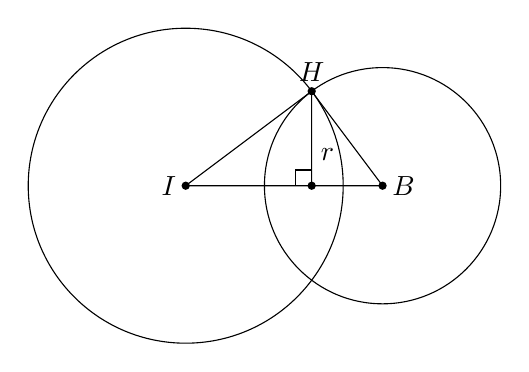
\begin{tikzpicture}[>=stealth,x=1cm,y=1cm,scale=1]
				\fill[black] (-1,0)node[left]{\normalsize $I$} circle (1.5pt);
				\fill[black] (1.5,0)node[right]{\normalsize $B$} circle (1.5pt);
				\fill[black] (0.6,1.2)node[above]{\normalsize $H$} circle (1.5pt);
				\fill[black] (0.6,0) circle (1.5pt);
				\draw(-1,0) circle (2cm);
				\draw(1.5,0) circle (1.5cm);
				\draw (-1,0)--(0.6,1.2)--(1.5,0)--cycle (0.6,0)--(0.6,1.2);
				\node at (0.8,0.4) {$ r $};
				\draw (0.6,0)--(0.6,0.2)--(0.4,0.2)--(0.4,0);
		\end{tikzpicture}}
	}
\end{ex}


\begin{ex}%[2H5V1-5]
	Trong không gian $Oxyz$, cho hai điểm $A(1;-1;3)$, $B(3;2;2)$. Biết rằng hai điểm $A$ và $B$ nằm khác phía so với mặt phẳng $ (\alpha)\colon ax+by+3z+d=0 $, với $ a $ và $ d $ là những tham số. Biết rằng tổng khoảng cách từ $ A $ và $ B $ đến $ (\alpha) $ lớn nhất. Giá trị nguyên dương lớn nhất của $ d $ là
	\shortans{$29$}
	\loigiai{
		\immini
		{Vì $ A $, $ B $ khác phía đối với $ (\alpha) $ nên gọi $I$ là giao điểm của đoạn thẳng $AB $ và $ (\alpha) $, gọi $ H $, $ K $ lần lượt là hình chiếu vuông góc của $ A $ và $ B $ trên mặt phẳng $ (\alpha) $, ta có 
			\begin{eqnarray*}
				T&=&\mathrm{d}\left(A,(\alpha)\right)+\mathrm{d}\left(B,(\alpha)\right)\\
				&=&AH+BK\\
				&\le & AI+ BI=AB.
			\end{eqnarray*}
			Dấu \lq\lq$=$\rq\rq\, xảy ra khi và chỉ khi $\heva{&\mathrm{d}\left(A,(\alpha)\right)=AI \\ & \mathrm{d}\left(B,(\alpha)\right)=BI} \Leftrightarrow AB \perp \left(\alpha\right)$.}
		{\begin{tikzpicture}[line join=round, line cap=round,scale=0.8]
				\path
				(2,2) coordinate (M)
				(9,2) coordinate (N)
				(0,0) coordinate (Q)
				($(N)+(Q)-(M)$) coordinate (P)
				(4,1) coordinate (I)
				(3,1) coordinate (H)
				(6,1) coordinate (K)
				(3,3) coordinate (A)
				(6,-3) coordinate (B)
				;
				\path[name path=ah] (A)--(H);
				%				\path[name path=ah] (A)--(H)--([turn]0:5cm);
				\path[name path=ab] (A)--(B);
				\path[name path=mn] (M)--(N);
				\path[name path=pq] (P)--(Q);
				\path[name path=bk] (B)--(K);
				\path[name intersections={of=ah and mn,by=E}];
				\path[name intersections={of=ab and mn,by=F}];
				\path[name intersections={of=ab and pq,by=G}];
				\path[name intersections={of=bk and pq,by=J}];
				\draw
				
				(M)--(E) (F)--(N)--(P)--(Q)--(M)
				(A)--(I)--(H)--cycle (G)--(B)--(J) (I)--(K)
				;
				\draw[dashed]
				(E)--(F) (I)--(G) (K)--(J)
				;
				\foreach \i/\g in {A/90,B/-90,I/60,H/180,K/0}
				{\draw[fill=black](\i) circle (1pt) ($(\i)+(\g:3mm)$) node[scale=1]{$\i$};}
				\draw pic[draw,,angle radius=9mm]{angle=P--Q--M};
				\draw pic["$\alpha$",-stealth,angle radius=9mm]{angle=P--Q--M};
		\end{tikzpicture}}
		\noindent
		Suy ra $T$ lớn nhất khi $ \left(\alpha\right) \perp AB$ hay $ \vec{AB}=(2;3;-1) $ là một véc-tơ pháp tuyến của $ (\alpha)$.\\
		Ta có $\vec{AB}$ cùng phương với $\vec{n}=(a;b;3)$ khi và chỉ khi
		\[\dfrac{a}{2}=\dfrac{b}{3}=\dfrac{3}{-1} \Rightarrow \heva{& a=-6 \\ & b=-9.}\]
		Phương trình $ (\alpha)\colon-6x-9y+3z+d=0$.\\
		Vì $ A $, $ B $ khác phía đối với $ (\alpha) $ nên 
		\[(-6+9+9+d)\cdot(-18-18+6+d)<0\Leftrightarrow-12<d<30.\]
		Vậy số nguyên $ d $ lớn nhất bằng $ 29$.
	}
\end{ex}



\begin{ex}%[2H5V1-3]
	Trong không gian $Oxyz$, cho hai điểm $A(2;4;1)$, $B(-1;1;3)$ và mặt phẳng $(P)\colon x-3y+2z-5=0$. Mặt phẳng $(Q)$ đi qua $A$, $B$ và vuông góc với $(P)$ có phương trình dạng $ax+by+cz+11=0$. Tổng $a+b+c$ bằng
	\shortans{$-5$}
	\loigiai
	{Ta có $\overrightarrow{AB}=(-3;-3;2)$, véc-tơ $\overrightarrow{n}=(1;-3;2)$ là véc-tơ pháp tuyến của $(P)$.\\
		Mặt phẳng $(Q)$ đi qua hai điểm $A$, $B$ và vuông góc với mặt phẳng $(P)$ nên nhận véc-tơ $\left[\overrightarrow{AB}, \overrightarrow{n}\right] = (0;8;12)$ làm véc-tơ pháp tuyến. Do đó phương trình $(Q)$ là
		$$8(y-4)+12(z-1)=0 \Leftrightarrow 2y+3z-11=0 \Leftrightarrow -2y-3z+11=0.$$
		Vậy $a=0$, $b=-2$, $c=-3$ và $a+b+c=-5$.}
\end{ex}


\begin{ex}%[2H5C1-7]
	Trong không gian $Oxyz$, cho hai điểm $A(2;1;0)$, $B(1;2;0)$ và điểm $M$ di động trên tia $Oz$. Gọi $H$, $K$ lần lượt là hình chiếu vuông góc của $A$ lên $OB$ và $MB$. Đường thẳng $HK$ cắt trục $Oz$ tại điểm $N$. Khi thể tích khối tứ diện $ABMN$ nhỏ nhất thì mặt phẳng $(AHK)$ có dạng $ax+by+cz-4=0$. Giá trị của $a+b+c$ bằng
	\par\shortans{$1$}
	\loigiai{
		\immini
		{Ta có $A(2;1;0)$, $B(1;2;0)$ $\Rightarrow A,~ B \in (Oxy)$.\\
			Có $\heva{&AK\perp MB\\&AH\perp OB;~AH\perp OM \Rightarrow AH \perp (OBM) \Rightarrow AH \perp MB}$ mà $AK\perp MB$ nên 
			$ MB \perp (AHK)$.\\
			Gọi $M(0;0;m)$, $(m>0)$ thuộc tia $Oz$ khi đó $\overrightarrow{MB}=(1;2;-m)$\\
			$\Rightarrow (AHK)\colon 1(x-2)+2(y-1)-mz=0$.\\
			$\Rightarrow N=HK \cap Oz =(AHK) \cap Oz \Rightarrow N\left(0;0;-\dfrac{4}{m}\right)$.\\
			Ta có
			\allowdisplaybreaks
			$\begin{aligned}[t]
				V_{ABMN}&=V_{M.OAB}+V_{N.OAB}=\dfrac{1}{3}S_{OAB}\cdot OM +\dfrac{1}{3}S_{OAB}\cdot ON\\
				&=\dfrac{1}{3}S_{OAB}(OM+ON)=\dfrac{1}{3}S_{OAB}\cdot MN
			\end{aligned}$\\
			Vì $S_{OAB}$ không đổi nên $V_{ABMN}$ nhỏ nhất khi và chỉ khi $MN$ nhỏ nhất.\\
			Ta có $MN=m+\dfrac{4}{m}\geq 2\sqrt{m\cdot \dfrac{4}{m}}=4$.\\
			Dấu bằng xảy ra khi $m=\dfrac{4}{m}\Rightarrow m=2$.\\
			Vậy $(AHK)\colon x+2y-2z-4=0 \Rightarrow a+b+c=1+2-2=1$.}
		{\begin{tikzpicture}[scale=1, font=\footnotesize, line join=round, line cap=round,>=stealth]
				\def\xmin{-2};\def\ymin{-3};\def\xmax{6};\def\ymax{5};
				\coordinate (O) at (0,0);
				\coordinate (B) at (2,-1);
				\coordinate (A) at (3,0);
				\coordinate (M) at (0,2);
				\coordinate (K) at ($(M)+2/5*(B)-2/5*(M)$);
				\coordinate (H) at ($(O)+1/4*(B)-1/4*(O)$);
				\coordinate (N) at (intersection of M--O and K--H);
				\draw (A)--(B)--(O)--(M)--cycle (M)--(B)--(N) (A)--(K)--(N)--(O);
				\draw [dashed] (O)--(A)--(H) (A)--(N);
				\draw[black] pic[draw, angle radius=2mm, angle eccentricity=1.5]{right angle=B--K--A};
				\draw[black] pic[draw, angle radius=2mm, angle eccentricity=1.5]{right angle=B--H--A};
				\foreach \t/\g in {O/180,B/-90,A/0,M/70,K/90,H/200,N/-90}{\draw[fill=white] (\t) circle (1pt) node[shift={(\g:7pt)},font=\scriptsize]{$\t$};}
		\end{tikzpicture}}
	}
\end{ex}


\Closesolutionfile{ans}

%\subsection{Phương trình đường thẳng}
\begin{name}
	{\tenchude}
	{TOÁN 12 - PHƯƠNG TRÌNH ĐƯỜNG THẲNG}
	{LỚP TOÁN THẦY PHÁT}
	{Thời gian: 90 phút - Không kể thời gian phát đề}
\end{name}
\Opensolutionfile{ans}[ans/ans-0-B15]
\caulc
%%==========Câu 23
\begin{ex} Trong không gian $Oxyz$, cho đường thẳng $d\colon \dfrac{x-3}{2}=\dfrac{y-4}{-5}=\dfrac{z+1}{3}$. Véc-tơ nào dưới đây là một véc-tơ chỉ phương của $d$?
	\choice
	{$\overrightarrow{u}_2=(2; 4;-1)$}
	{\True $\overrightarrow{u}_1=(2;-5; 3)$}
	{$\overrightarrow{u}_3=(2; 5; 3)$}
	{$\overrightarrow{u}_4=(3; 4; 1)$}
	\loigiai{Véc-tơ chỉ phương của $d$ là $\overrightarrow{u}_1=(2;-5; 3)$.
	}
\end{ex}
%%==========Câu 24
\begin{ex}Trong không gian $Oxyz$, đường thẳng $d\colon \heva{&x=2-t \\&y=1+2 t \\&z=3+t}$ có một véc-tơ chỉ phương là
	\choice
	{$\overrightarrow{u}_1=(-1; 2; 3)$}
	{$\overrightarrow{u}_3=(2; 1; 3)$}
	{\True $\overrightarrow{u}_4=(-1; 2; 1)$}
	{$\overrightarrow{u}_2=(2; 1; 1)$}
	\loigiai{$d\colon \heva{&x=2-t \\&y=1+2 t \\&z=3+t}$ có một véc-tơ chỉ phương là $\overrightarrow{u}_4=(-1; 2; 1)$.}
\end{ex}
%%==========Câu 25
\begin{ex}Trong không gian với hệ toạ độ $Oxyz$, cho hai điểm $A(1; 1; 0)$ và $B(0;1;2)$. Véc-tơ nào dưới đây là một véc-tơ chỉ phương của đường thẳng $AB$
	\choice
	{$\overrightarrow{d}=(-1; 1; 2)$}
	{$\overrightarrow{a}=(-1; 0;-2)$}
	{\True $\overrightarrow{b}=(-1; 0; 2)$}
	{$\overrightarrow{c}=(1; 2; 2)$}
	\loigiai{
	Ta có $\overrightarrow{AB}=(-1; 0; 2)$ suy ra đường thẳng $AB$ có vectơ chỉ phương là $\overrightarrow{b}=(-1; 0; 2)$.}
\end{ex}
%%==========Câu 26
\begin{ex}Trong không gian với hệ toạ độ $Oxyz$, cho điểm $M(1; 2; 3)$. Gọi $M_1$, $M_2$ lần lượt là hình chiếu vuông góc của $M$ lên các trục $Ox$, $Oy$. Véc-tơ nào dưới đây là một véc-tơ chỉ phương của đường thẳng $M_1M_2$
	\choice
	{$\overrightarrow{u}_4=(-1; 0; 2)$}
	{$\overrightarrow{u}_1=(0; 2; 0)$}
	{\True $\overrightarrow{u}_2=(-1; 2; 0)$}
	{$\overrightarrow{u}_3=(1; 0; 0)$}
	\loigiai{
	$M_1$ là hình chiếu của $M$ lên trục $Ox\Rightarrow M_1(1;0;0)$.\\
	$M_2$ là hình chiếu của $M$ lên trục $Oy\Rightarrow M_2(0;2;0)$.\\
	Khi đó, $\overrightarrow{M_1M_2}=(-1;2;0)$ là một véc-tơ chỉ phương của $M_1M_2$.}
\end{ex}
%%==========Câu 27
\begin{ex}Trong không gian $Oxyz$, cho hai điểm $M(1; 2; 1)$ và $N(3; 1;-2)$. Đường thẳng $MN$ có phương trình là
	\choice
	{$\dfrac{x+1}{4}=\dfrac{y+2}{3}=\dfrac{z+1}{-1}$}
	{\True $\dfrac{x-1}{2}=\dfrac{y-2}{-1}=\dfrac{z-1}{-3}$}
	{$\dfrac{x-1}{4}=\dfrac{y-2}{3}=\dfrac{z-1}{-1}$}
	{$\dfrac{x+1}{2}=\dfrac{y+2}{-1}=\dfrac{z+1}{-3}$}
	\loigiai{
	Ta có $\overrightarrow{MN}=(2;-1;-3)$.\\
	Đường thẳng $MN$ đi qua điểm $M(1; 2; 1)$ và nhận véc-tơ $\overrightarrow{MN}=(2;-1;-3)$ làm véc-tơ chỉ phương có phương trình là $\dfrac{x-1}{2}=\dfrac{y-2}{-1}=\dfrac{z-1}{-3}$.}
\end{ex}
%%==========Câu 28
\begin{ex}Trong không gian $Oxyz$, cho hai điểm $M(1; 0; 1)$ và $N(3; 2;-1)$. Đường thẳng $MN$ có phương trình tham số là
	\choice
	{$\heva{&x=1+2t \\&y=2 t \\&z=1+t}$}
	{$\heva{&x=1+t \\&y=t \\&z=1+t}$}
	{$\heva{&x=1-t \\&y=t \\&z=1+t}$}
	{\True $\heva{&x=1+t \\&y=t \\&z=1-t}$}
	\loigiai{
	Đường thẳng $MN$ nhận $\overrightarrow{MN}=(2; 2;-2)$ hoặc $\overrightarrow{u}=(1; 1;-1)$ là véc-tơ chỉ phương.\\
	Đường thẳng $MN$ đi qua điểm điểm $M(1; 0; 1)$ và nhận $\overrightarrow{u}=(1; 1;-1)$ là véc-tơ chỉ phương có phương trình tham số là $\heva{&x=1+t \\&y=t \\&z=1-t.}$}
\end{ex}
%%==========Câu 29
\begin{ex}Trong không gian tọa độ $Oxyz$, phương trình nào dưới đây là phương trình chính tắc của đường thẳng $d\colon\heva{&x=1+2t \\&y=3t \\&z=-2+t}(t\in \mathbb{R})$?
	\choice
	{$\dfrac{x+1}{2}=\dfrac{y}{3}=\dfrac{z-2}{1}$}
	{$\dfrac{x-1}{1}=\dfrac{y}{3}=\dfrac{z+2}{-2}$}
	{$\dfrac{x+1}{2}=\dfrac{y}{3}=\dfrac{z-2}{-2}$}
	{\True $\dfrac{x-1}{2}=\dfrac{y}{3}=\dfrac{z+2}{1}$}
	\loigiai{
	Do đường thẳng $d\colon \heva{&x=1+2t \\&y=3t \\&z=-2+t}$ đi qua điểm $M(1; 0;-2)$ và có véc-tơ chỉ phương\\ $\overrightarrow{u}=(2; 3; 1)$ nên có phương trình chính tắc là $\dfrac{x-1}{2}=\dfrac{y}{3}=\dfrac{z+2}{1}$.}
\end{ex}
%%==========Câu 30
\begin{ex}
	Trong không gian với hệ tọa độ $Oxyz$, cho hai điểm $M(1;-2; 1)$, $N(0; 1; 3)$. Phương trình đường thẳng qua hai điểm $M$, $N$ là
	\choice
	{$\dfrac{x+1}{-1}=\dfrac{y-2}{3}=\dfrac{z+1}{2}$}
	{$\dfrac{x+1}{1}=\dfrac{y-3}{-2}=\dfrac{z-2}{1}$}
	{\True $\dfrac{x}{-1}=\dfrac{y-1}{3}=\dfrac{z-3}{2}$}
	{$\dfrac{x}{1}=\dfrac{y-1}{-2}=\dfrac{z-3}{1}$}
	\loigiai{
	Ta có $\overrightarrow{MN}=(-1; 3; 2)$.\\
	Đường thẳng $MN$ đi qua $N(0; 1; 3)$ và nhận $\overrightarrow{MN}=(-1; 3; 2)$ làm véc-tơ chỉ phương có phương trình là
	$\dfrac{x}{-1}=\dfrac{y-1}{3}=\dfrac{z-3}{2}$.}
\end{ex}
%%==========Câu 31
\begin{ex}Trong không gian $Oxyz$, cho đường thẳng $d$ đi qua điểm $M(3;-1; 4)$ và có một véc-tơ chỉ phương $\overrightarrow{u}=(-2; 4; 5)$. Phương trình của $d$ là
	\choice
	{$\heva{&x=-2+3t \\&y=4-t \\&z=5+4t}$}
	{$\heva{&x=3+2t \\&y=-1+4t \\&z=4+5t}$}
	{$\heva{&x=3-2t \\&y=1+4t \\&z=4+5t}$}
	{\True $\heva{&x=3-2t \\&y=-1+4t \\&z=4+5t}$}
	\loigiai{
	Đường thẳng $d$ đi qua điểm $M(3;-1; 4)$ và có một véc-tơ chỉ phương $\overrightarrow{u}=(-2; 4; 5)$. Phương trình của $d$ là $\heva{&x=3-2 t \\ &y=-1+4t \\&z=4+5t}(t\in\mathbb{R})$.}
\end{ex}
%%==========Câu 32
\begin{ex}
	Trong không gian $Oxyz$, đường thẳng $Oy$ có phương trình tham số là
	\choice
	{$\heva{&x=t\\&y=t\\&z=t}(t\in \mathbb{R})$}
	{\True $\heva{&x=0\\&y=2+t\\&z=0}(t\in \mathbb{R})$}
	{$\heva{&x=0\\&y=0\\&z=t}(t\in \mathbb{R})$}
	{$\heva{&x=t\\&y=0\\&z=0}(t\in \mathbb{R})$}
	\loigiai{Đường thẳng $Oy$ đi qua điểm $A(0;2;0)$ và nhận véc-tơ đơn vị $\overrightarrow{j}=(0;1;0)$ làm véc-tơ chỉ phương nên có phương trình tham số là $\heva{&x=0+0\cdot t\\&y=2+1\cdot t\\&z=0+0\cdot t}(t\in \mathbb{R})\Leftrightarrow \heva{&x=0\\&y=2+t\\&z=0}(t\in\mathbb{R})$.
	}
\end{ex}
%%==========Câu 33
\begin{ex}Trong không gian $Oxyz$, cho điểm $A(1; 2; 3)$ và đường thẳng $d\colon \dfrac{x-3}{2}=\dfrac{y-1}{1}=\dfrac{z+7}{-2}
	$. Đường thẳng đi qua $A$, vuông góc với $d$ và cắt trục $Ox$ có phương trình là
	\choice
	{$\heva{&x=-1+2t \\&y=-2t \\&z=t}$}
	{$\heva{&x=1+t \\&y=2+2t \\&z=3+3t}$}
	{\True $\heva{&x=-1+2t \\&y=2t \\&z=3t}$}
	{$\heva{&x=1+t \\&y=2+2t \\&z=3+2t}$}
	\loigiai{
	Gọi $\Delta$ là đường thẳng cần tìm.\\
	Gọi $M=\Delta \cap Ox$. Suy ra $M\ (a; 0; 0)$.\\
	$\overrightarrow{AM}=(a-1;-2;-3)$.\\
	Đường thẳng $d$ có véc-tơ chỉ phương $\overrightarrow{u}_d=(2; 1;-2)$.\\
	Vì $\Delta \perp d$ nên $\overrightarrow{AM}\cdot \overrightarrow{u}_d=0 \Leftrightarrow 2a-2-2+6=0 \Leftrightarrow a=-1$.\\
	Vậy $\Delta$ qua $M(-1; 0; 0)$ và có véc-tơ chỉ phương $\overrightarrow{AM}=(-2;-2;-3)=-(2; 2; 3)$ nên $\Delta$ có phương trình: $\heva{&x=-1+2t \\&y=2t \\&z=3t}(t\in \mathbb{R})$.
	}
\end{ex}
%%==========Câu 34
\begin{ex}Trong không gian $Oxyz$, cho các điểm $A(1; 0; 2)$, $B(1; 2; 1)$, $C(3; 2; 0)$ và $D(1; 1; 3)$. Đường thẳng đi qua $A$ và vuông góc với mặt phẳng $(BCD)$ có phương trình là
	\choice
	{$\heva{&x=1-t \\&y=4t \\&z=2+2t}$}
	{$\heva{&x=1+t \\&y=4 \\&z=2+2t}$}
	{\True $\heva{&x=2+t \\&y=4+4t \\&z=4+2t}$}
	{$\heva{&x=1-t \\&y=2-4t \\&z=2-2t}$}
	\loigiai{
	Đường thẳng đi qua $A$ và vuông góc với mặt phẳng $(BCD)$ nhận véc-tơ pháp tuyến của $(BCD)$ là véc-tơ chỉ phương.\\
	Ta có $\overrightarrow{BC}=(2; 0;-1)$, $\overrightarrow{BD}=(0;-1; 2)$.\\
	$\Rightarrow \overrightarrow{u}_d=\overrightarrow{n}_{\left( BCD\right) }=\left[ \overrightarrow{BC}; \overrightarrow{BD}\right] =(-1;-4;-2)$.\\
	Thay điểm $A(1; 0; 2)$ vào phương trình $\heva{&x=2+t \\&y=4+4t \\&z=4+2t}$ ta có $\heva{&1=2+t \\ &0=4+4 t \\&2=4+2 t} \Leftrightarrow t=-1.$\\
	Vậy đường thẳng đi qua $A$ và vuông góc với mặt phẳng $(BCD)$ có phương trình là $\heva{&x=2+t \\&y=4+4t \\&z=4+2t.}$
	}
\end{ex}
\Closesolutionfile{ans}
%\indapan{6}{ans/ans-0-B15}
\cauds
\Opensolutionfile{ans}[ans/ans-0-B15-DS]
%%==========Câu 35
\begin{ex}
	Trong không gian $Oxyz$, cho mặt phẳng $(\alpha)\colon x+y-z+6=0$ và đường thẳng $d\colon \dfrac{x-1}{2}=\dfrac{y+4}{3}=\dfrac{z}{5}$.
	\choiceTF
	{\True Mặt phẳng $(\alpha)$ có véc-tơ pháp tuyến $\overrightarrow{n}=(1;1;-1)$}
	{\True $d\parallel (\alpha)$}
	{Đường thẳng đi qua $A$ và vuông góc với $(\alpha)$ có phương trình $\heva{&x=1+t\\&y=-4+t\\&z=t}(t\in\mathbb{R})$}
	{Hình chiếu vuông góc của $d$ lên $(\alpha)$ có phương trình là $\dfrac{x}{2}=\dfrac{y+5}{3}=\dfrac{z+1}{5}$}
	\loigiai{
	\begin{itemchoice}
	\itemch Đúng. Mặt phẳng $(\alpha)\colon x+y-z+6=0$ có véc-tơ pháp tuyến $\overrightarrow{n}=(1;1;-1)$.
	\itemch Đúng.\\ Mặt phẳng $(\alpha)\colon x+y-z+6=0$ có véc-tơ pháp tuyến $\overrightarrow{n}=(1;1;-1)$. \\Đường thẳng $d\colon \dfrac{x-1}{2}=\dfrac{y+4}{3}=\dfrac{z}{5}$ có véc-tơ chỉ phương $\overrightarrow{u}=(2;3;5)$.\\ Vì $\overrightarrow{n}\cdot\overrightarrow{u}=1\cdot2+1\cdot3-1\cdot5=0$ nên $d\parallel (\alpha)$.
	\itemch Sai. \\
	Ta có $(\alpha)\colon x+y-z+6=0$ nên $\overrightarrow{n}_{\alpha}=\left(1;1;-1 \right)$.\\	Lấy $A(1;-4;0)\in d$.\\ Gọi $\Delta$ là đường thẳng đi qua $A(1;-4;0)$ và vuông góc với $(\alpha)$ nên $\overrightarrow{u}_{\Delta}=\left(1;1;-1 \right) $.\\ Suy ra phương trình tham số của đường thẳng $\Delta$ là $\heva{&x=1+t\\&y=-4+t\\&z=-t}(t\in \mathbb{R})$.
	\itemch Sai. \\
	Đường thẳng $d\colon \dfrac{x-1}{2}=\dfrac{y+4}{3}=\dfrac{z}{5}$ có $\overrightarrow{u}_d=(2;3;5)$.\\
	Gọi $d'$ là hình chiếu vuông góc của $d$ trên $(\alpha)\Rightarrow d'\parallel d$.\\
	Vì $d'\parallel d$ nên $d'$ nhận $\overrightarrow{u}_{d'}=\overrightarrow{u}_{\Delta}=\left(2;3;5\right)$ làm véc-tơ chỉ phương.\\
	Gọi $A'$ là hình chiếu của $A$ lên $(\alpha)$ thì $A'=\Delta \cap (\alpha)\Rightarrow A'(0;-5;1)$.\\Đường thẳng $d'$ đi qua $A'(0;-5;1)$, nhận $\overrightarrow{u}_{d'}=(2;3;5)$ làm véc-tơ chỉ phương có phương trình là $\dfrac{x}{2}=\dfrac{y+5}{3}=\dfrac{z-1}{5}$.
	\end{itemchoice}
	}
\end{ex}
%%==========Câu 36
\begin{ex}
	Trong không gian $Oxyz$, cho $M(1;0;1)$ và đường thẳng $(\Delta)\colon\dfrac{x}{1}=\dfrac{y}{2}=\dfrac{z}{3}$
	\choiceTF
	{$M\in (\Delta)$}
	{\True $(\Delta)$ có véc-tơ chỉ phương $\overrightarrow{u}=(1;2;3)$}
	{\True Phương trình tham số của $(\Delta)\colon \heva{&x=t\\&y=2t\\&z=3t}(t\in \mathbb{R})$}
	{Toạ độ hình chiếu của $M$ lên đường thẳng $(\Delta)$ là $N\left(2;4;6\right)$}
	\loigiai{
	\begin{itemchoice}
	\itemch Sai. Ta có $\dfrac{1}{1}\neq \dfrac{0}{2}\neq \dfrac{1}{3}$ nên $M\notin (\Delta)$.
	\itemch Đúng. $(\Delta)\colon\dfrac{x}{1}=\dfrac{y}{2}=\dfrac{z}{3}$ có véc-tơ chỉ phương $\overrightarrow{u}=(1;2;3)$.
	\itemch Đúng. $(\Delta)\colon\dfrac{x}{1}=\dfrac{y}{2}=\dfrac{z}{3}$ đi qua điểm $O\left(0;0;0 \right)$ và có véc-tơ chỉ phương $\overrightarrow{u}=(1;2;3)$ nên có phương trình tham số của $(\Delta)\colon \heva{&x=t\\&y=2t\\&z=3t}(t\in \mathbb{R})$.
	\itemch Sai.\\ Gọi $N(t;2t;3t)\in \Delta$ là hình chiếu vuông góc của $M$ lên $\Delta$, khi đó \allowdisplaybreaks\begin{eqnarray*}
	&&\overrightarrow{MN}\cdot \overrightarrow{u}=0\\
	&\Leftrightarrow&(t-1)+(2t-0)\cdot2+(3t-1)\cdot3=0\\
	&\Leftrightarrow&14t-4=0\\
	&\Leftrightarrow& t=\dfrac{2}{7}\\
	&\Rightarrow& N\left( \dfrac{2}{7};\dfrac{4}{7};\dfrac{6}{7}\right).
	\end{eqnarray*}
	\end{itemchoice}
	}
\end{ex}
%%==========Câu 37
\begin{ex}
	Trong không gian $Oxyz$, cho đường thẳng $d\colon \dfrac{x+1}{1}=\dfrac{y+3}{2}=\dfrac{z+2}{2}$ và điểm $A(3 ; 2 ; 0)$. 
	\choiceTF
	{\True $M(-1;-3;-2)\in d$}
	{\True $\overrightarrow{u}=(1;2;2)$ là véc-tơ chỉ phương của $d$}
	{Toạ độ hình chiếu của $A$ lên đường thẳng $d$ là $H(2;2;1)$}
	{Điểm đối xứng của điểm $A$ qua đường thẳng $d$ có tọa độ là $A'(1;0;4)$}
	\loigiai{
	\begin{itemchoice}
	\itemch Đúng. Đường thẳng $d\colon \dfrac{x+1}{1}=\dfrac{y+3}{2}=\dfrac{z+2}{2}$ nên $M(-1;-3;-2)\in d$.
	\itemch Đúng. Đường thẳng $d\colon \dfrac{x+1}{1}=\dfrac{y+3}{2}=\dfrac{z+2}{2}$ nên $\overrightarrow{u}=(1;2;2)$ là véc-tơ chỉ phương của $d$.
	\itemch Sai. \\Gọi $(P)$ là mặt phẳng đi qua $A$ và vuông góc với đường thẳng $d$.\\ Phương trình của mặt phẳng
	$(P)$ là \allowdisplaybreaks\begin{eqnarray*}
	1\cdot(x-3)+2\cdot(y-2)+2\cdot(z-0)=0 \Leftrightarrow x+2y+2z-7=0.
	\end{eqnarray*}
	Gọi $H$ là hình chiếu của $A$ lên đường thẳng $d$, khi đó $H=d \cap(P)$.\\
	Suy ra $H \in d \Rightarrow H(-1+t ;-3+2 t ;-2+2 t)$.\\ Mặt khác $H \in(P) \Rightarrow-1+t-6+4 t-4+4 t-7=0\Rightarrow t=2$. Vậy $H(1 ; 1 ; 2)$.
	\itemch Sai. \\Gọi $A'$ là điểm đối xứng với $A$ qua đường thẳng $d$, khi đó $H$ là trung điểm của $AA'$ nên ta có hệ phương trình
	\begin{eqnarray*}
	\heva{&x_A+x_A'=2x_H\\&y_A+y_A'=2y_H\\&z_A+z_A'=2z_H}\Leftrightarrow\heva{&x_A'=2x_H-x_A=2\cdot1-3=-1\\&y_A'=2y_H-y_A=2\cdot1-2=0\\&z_A'=2z_H-z_A=2\cdot2-0=4.}
	\end{eqnarray*} Do đó, $A'(-1 ; 0 ; 4)$.
	\end{itemchoice}
	}
\end{ex}
%%==========Câu 38
\begin{ex}
	Trong không gian $Oxyz$, cho mặt phẳng $(P)\colon 6x-2y+z-35=0$ và điểm $A(-1;3;6)$. 
	\choiceTF
	{\True $\overrightarrow{n}=(6;-2;-1)$ là véc-tơ pháp tuyến của $(P)$}
	{\True $A(-1;3;6)\notin (P)$}
	{\True Toạ độ điểm đối xứng với $A$ qua $(P)$ là $A'(11;-1;8)$}
	{Độ dài $OA'=186$}
	\loigiai{
	\begin{itemchoice}
	\itemch Đúng. Mặt phẳng $(P)\colon 6x-2y+z-35=0$ có $\overrightarrow{n}=(6;-2;-1)$ là véc-tơ pháp tuyến.
	\itemch Đúng. Ta có $6\cdot(-1)-2\cdot3+6-35=-41\neq 0$ nên $A\notin (P)$.
	\itemch Đúng. \\ $A'$ đối xứng với $A$ qua $(P)$ nên $AA'$ vuông góc với $(P)$.\\
	Suy ra phương trình đường thẳng $AA'\colon\heva{&x=-1+6 t \\&y=3-2 t \\&z=6+t}(t\in \mathbb{R})$.\\
	Gọi $H$ là giao điểm của $AA'$ và mặt phẳng $(P) \Rightarrow H(-1+6t;3-2t;6+t)$.
	\allowdisplaybreaks\begin{eqnarray*}
	\text{ Do }	H \in (P)&\Rightarrow& 6\cdot(-1+6 t)-2\cdot(3-2 t)+1\cdot(6+t)-35=0\\
	&\Rightarrow& 41 t-41=0\\
	&\Rightarrow& t=1 \\
	&\Rightarrow& H(5 ; 1 ; 7).
	\end{eqnarray*}
	$A'$ đối xứng với $A$ qua $(P)$ nên $H$ là trung điểm của $AA'$. Do đó, ta có hệ phương trình
	\begin{eqnarray*}
	\heva{&x_A+x_A'=2x_H\\&y_A+y_A'=2y_H\\&z_A+z_A'=2z_H}\Leftrightarrow\heva{&x_A'=2x_H-x_A=2\cdot5+1=11\\&y_A'=2y_H-y_A=2\cdot1-3=-1\\&z_A'=2z_H-z_A=2\cdot7-6=8.}
	\end{eqnarray*}
	Do đó, $A'(11 ;-1 ; 8)$.
	\itemch Sai. Ta có $A'(11 ;-1 ; 8)\Rightarrow O A'=\sqrt{11^2+(-1)^2+8^2}=\sqrt{186}$.
	\end{itemchoice}
	}
\end{ex}
\Closesolutionfile{ans}
%\indapan{3}{ans/ans-0-B15-DS}
\Opensolutionfile{ans}[ans/ans-0-B15-KQ]
\caukq
%%==========Câu 39
\begin{ex}
	Trong không gian $Oxyz$, khoảng cách từ $M(2;-4;-1)$ tới đường thẳng $\Delta \colon \heva{&x=t\\&y=2-t\\&z=3+2t}$ bằng bao nhiểu? (\textit{kết quả làm tròn đến hàng phần trăm}).
	\shortans{$7{,}48$}
	\loigiai{
	Đường thẳng $\Delta$ đi qua $N(0;2;3)$, có véc-tơ chỉ phương $\overrightarrow{u}=(1;-1;2)$.\\
	$\overrightarrow{MN}=(-2;6;4)$.\\ $\left[\overrightarrow{MN},\overrightarrow{u}\right]=\left(16;8;-4\right)$.\\
	$\mathrm{\,d}(M,\Delta)=\dfrac{\left|\left[\overrightarrow{MN},\overrightarrow{u}\right] \right| }{\left|\overrightarrow{u} \right| }=\dfrac{\sqrt{336}}{\sqrt{6}}=2\sqrt{14}\approx7{,}48$.
	}
\end{ex}
%%==========Câu 40
\begin{ex}
	Trong không gian $Oxyz$, cho đường thẳng $d\colon \dfrac{x+1}{2}=\dfrac{y}{1}=\dfrac{z-2}{-1}$ và hai điểm $A(-1 ; 3 ; 1)$; $B(0 ; 2 ;-1)$. Gọi $C(m ; n ; p)$ là điểm thuộc đường thẳng $d$ sao cho diện tích tam giác $ABC$ bằng $2\sqrt{2}$. Tính giá trị của tổng $m+n+p$.
	\shortans{$3$}
	\loigiai{
	Phương trình tham số của đường thẳng $d\colon\heva{&x=-1+2 t \\&y=t \\&z=2-t}(t\in \mathbb{R})$.\\
	Vì $C \in d\colon\heva{&x=-1+2 t \\&y=t \\&z=2-t} \Rightarrow C(-1+2t ; t;2-t)$.\\
	Ta có $\overrightarrow{AB}=(1 ;-1 ;-2)$; $\overrightarrow{AC}=(-1+2t;t;2-t) \Rightarrow\left[\overrightarrow{AB},\overrightarrow{AC}\right]=(3t-7;-3t-1; 3t-3)$.\\
	Diện tích tam giác $ABC$ là $S_{ABC}=\dfrac{1}{2}\cdot\left| \left[ \overrightarrow{AB}, \overrightarrow{AC}\right] \right| =\dfrac{1}{2} \sqrt{27t^2-54t+59}$.\\
	$S_{ABC}=2 \sqrt{2} \Leftrightarrow \dfrac{1}{2} \sqrt{27t^2-54t+59}=2\sqrt{2} \Leftrightarrow t=1 \Rightarrow C(1 ; 1 ; 1) \Rightarrow m+n+p=3$.}
\end{ex}
%%==========Câu 41
\begin{ex}
	Trong không gian với hệ trục tọa độ $Oxyz$. Gọi $M(a;b;c)$ thuộc đường thẳng $\Delta\colon\dfrac{x}{1}=\dfrac{y-1}{2}=\dfrac{z+2}{3}$. Biết điểm $M$ có tung độ âm và cách mặt phẳng $(Oyz)$ một khoảng bằng $2$. Xác định giá trị $T=a+b+c$.
	\par\shortans{$-13$}
	\loigiai{
	$M \in \Delta \Rightarrow M(t;1+2t;-2+3t)$.\\
	Ta có $\mathrm{\,d}(M ;(Oyz))=|t|=2 \Leftrightarrow\hoac{&t=2 \Rightarrow y_M=1+2t=5 \\ &t=-2 \Rightarrow y_M=1+2t=-3.}$\\
	Suy ra $t=-2$ (vì $M$ có tung độ âm). Do đó $M(-2;-3;-8)$.\\
	Vậy $a=-2$; $b=-3$; $c=-8\Rightarrow T=a+b+c=-13$.
	}
\end{ex}
%%==========Câu 42
\begin{ex}
	Trong không gian $Oxyz$, giao điểm của mặt phẳng $(P)\colon 3x+5y-z-2=0$ và đường thẳng $\Delta\colon \dfrac{x-12}{4}=\dfrac{y-9}{3}=\dfrac{z-1}{1}$ là điểm $M\left(x_0;y_0;z_0\right)$. Tính giá trị của tổng $x_0+y_0+z_0$.
	\shortans{$-2$}
	\loigiai{\allowdisplaybreaks
	\begin{eqnarray*}
	&& M \in \Delta \Rightarrow M(12+4 t ; 9+3 t ; 1+t) . \\
	&& M \in(P) \Leftrightarrow 3\cdot(12+4 t)+5\cdot(9+3 t)-(1+t)-2=0 \Leftrightarrow t=-3 . \\
	&& M(0 ; 0 ;-2) \Rightarrow x_0+y_0+z_0=-2.
	\end{eqnarray*}
	}
\end{ex}
%%==========Câu 43
\begin{ex}
	Trong không gian với hệ tọa độ $Oxyz$, cho mặt phẳng $(P)\colon x-2y+2z-3=0$ và mặt cầu $(S)$ tâm $I(5 ;-3 ; 5)$, bán kính $R=2 \sqrt{5}$. Từ một điểm $A$ thuộc mặt phẳng $(P)$ kẻ một đường thẳng tiếp xúc với mặt cầu $(S)$ tại $B$. Tính $OA$ biết $AB=4$ (\textit{kết quả làm tròn đến hàng phần chục}).
	\shortans{$3{,}3$}
	\loigiai{
	Khoảng cách từ điểm $I$ đến $(P)$ là $\mathrm{\,d}(I ;(P))=\dfrac{\left| 5-2 \cdot(-3)+2 \cdot 5-3\right| }{\sqrt{1^2+(-2)^2+2^2}}=6$.\\
	$A B$ tiếp xúc với $(S)$ tại $B$ nên tam giác $A I B$ vuông tại $\mathrm{B}$, do đó ta có
	\begin{eqnarray*}
	I A=\sqrt{I B^2+A B^2}=\sqrt{R^2+A B^2}=\sqrt{\left( 2 \sqrt{5}\right)^2+4^2}=6=\mathrm{\,d}(I ;(P))
	\end{eqnarray*}
	$\Rightarrow A$ là hình chiếu của $I$ lên $(P)$.\\
	Đường thẳng $IA$ đi qua $I(5 ;-3 ; 5)$ có véc-tơ chỉ phương $\overrightarrow{u}=\overrightarrow{n}_{(P)}=(1 ;-2 ; 2)$ có phương trình $\heva{&x=5+t \\&y=-3-2t \\&z=5+2t.}(t\in \mathbb{R})$\\
	Ta có \allowdisplaybreaks\begin{eqnarray*}
	&&A=IA \cap(P)\\
	& \Rightarrow& 5+t-2\cdot(-3-2t)+2\cdot(5+2t)-3=0\\
	& \Rightarrow& t=-2 \\
	&\Rightarrow& A(3 ; 1 ; 1)\\
	& \Rightarrow& OA=\sqrt{11}\approx 3{,}3.
	\end{eqnarray*}}
\end{ex}
%%==========Câu 44
\begin{ex}
	Trong không gian với hệ tọa độ $Oxyz$, cho hai điểm $A(4;6;2)$ và $B(2;-2;0)$ và mặt phẳng $(P)\colon x+y+z=0$. Xét đường thẳng $d$ thay đổi thuộc $(P)$ và đi qua $B$, gọi $H$ là hình chiếu vuông góc của $A$ trên $d$. Biết rằng khi $d$ thay đổi thì $H$ thuộc một đường tròn cố định. Tính bán kính $R$ của đường tròn đó (\textit{kết quả làm tròn đến hàng phần trăm}).
	\shortans{$2{,}45$}
	\loigiai{
	\begin{center}
	\begin{tikzpicture}[scale=1,>=stealth, font=\footnotesize, line join=round, line cap=round]
	\def\d{7}
	\def\r{3.5}
	\path (0:0) coordinate (V)
	++(0:\d) coordinate (B')
	++(50:\r) coordinate (N)
	($(V)+(N)-(B')$) coordinate (M)	
	($(V)!1/6!(N)$) coordinate (K)node[above]{$d$}
	($(V)!4/5!(N)$) coordinate (L)
	($(K)!1/3!(L)$) coordinate (H)
	($(H)!.5!(L)$) coordinate (B)
	($(H)!0.5!120:(B)$) coordinate (A')
	($(A')!2.5!135:(H)$) coordinate (A)
	;
	\draw (V)--(B')--(N)--(M)--cycle (K)--(L) (A)--(A')--(H)--cycle (A')--(B);
	\draw pic[draw,angle radius=2mm]{right angle=B--H--A};
	\draw pic[draw,angle radius=2mm]{right angle=H--A'--A};
	\draw pic[draw,"$P$",angle radius=6mm]{angle=N--B'--V};
	\foreach \x/ \goc in {H/-30,B/-30,A'/180,A/0} 
	\fill (\x) circle (1pt)	
	($(\x)+(\goc:3mm)$) node {$\x$};
	\end{tikzpicture}
	\end{center}
	Dễ thấy $B \in(P)$.\\
	Gọi $A'$ là hình chiếu của $A$ trên $(P)$, $A'$ cố định.
	Ta có 
	\begin{eqnarray*}
	\heva{&AA'\perp d \\
	&AH \perp d} \Rightarrow d \perp\left(AA'H\right) \Rightarrow d \perp A'H \Rightarrow \widehat{A'HB}=90^{\circ}.
	\end{eqnarray*}
	Suy ra khi $d$ thay đổi điểm $H$ luôn thuộc đường tròn đường kính $A'B$ cố định.\\
	Trước hết ta viết phương trình đường thẳng $AA'$ qua $A$ và vuông góc với $\left( P\right) $ nên nhận
	$\overrightarrow{n}_{\left(P\right) }=\left( 1 ; 1 ; 1\right) $ là một véc-tơ phương có phương trình $\heva{&x=4+t \\ &y=6+t \\ &z=2+t.}$
	\begin{eqnarray*}
	A'\in A A^{\prime} 
	&\Rightarrow& A^{\prime}(4+t ; 6+t ; 2+t) \\
	A' \in(P)
	& \Rightarrow& 4+t+6+t+2+t=0 \\
	& \Leftrightarrow& 3t+12=0\\
	& \Leftrightarrow& t=-4\\
	& \Leftrightarrow& A'(0 ; 2 ;-2).
	\end{eqnarray*}
	Khi đó $A'B=\sqrt{(2-0)^2+(-2-2)^2+(0+2)^2}=2 \sqrt{6}$.\\
	Vậy $H$ luôn thuộc đường tròn cố định có bán kính $R=\dfrac{A'B}{2}=\sqrt{6}\approx 2{,}45$.
	}
\end{ex}
\Closesolutionfile{ans}

% %\subsection{Phương trình mặt cầu}
\begin{name}
	{\tenchude}
	{TOÁN 12 - GÓC VÀ KHOẢNG CÁCH TRONG KHÔNG GIAN}
	{LỚP TOÁN THẦY PHÁT}
	{Thời gian: 90 phút - Không kể thời gian phát đề}
\end{name}
\Opensolutionfile{ans}[ans/ans-2-B16-De2]
\caulc
\begin{ex}%[Nguyễn Tuấn, dự án sáng tác đề 12 theo chủ đề]%[2H5H2-7]
	Cho hai mặt phẳng $(P_1)\colon A_1x+B_1y+C_1z+D_1=0$ $(A_1^2+B_1^2+C_1^2\ne 0)$ và \break $(P_2) \colon A_2x+B_2y+C_2z+D_2=0$ $(A_2^2+B_2^2+C_2^2\ne 0)$. Gọi $\varphi$ là góc giữa hai mặt phẳng $(P_1)$ và $(P_2)$. Hãy chọn khẳng định đúng?
	\choice
	{$\cos \varphi =\dfrac{\left|A_1A_2+B_1B_2+C_1C_2\right|}{(A_1^2+B_1^2+C_1^2)\cdot (A_2^2+B_2^2+C_2^2)}$}
	{\True $\cos \varphi =\dfrac{\left|A_1A_2+B_1B_2+C_1C_2\right|}{\sqrt{A_1^2+B_1^2+C_1^2}\cdot \sqrt{A_2^2+B_2^2+C_2^2}}$}
	{$\cos \varphi =\dfrac{A_1A_2+B_1B_2+C_1C_2}{(A_1^2+B_1^2+C_1^2)\cdot(A_2^2+B_2^2+C_2^2)}$}
	{$\cos \varphi =\dfrac{A_1A_2+B_1B_2+C_1C_2}{\sqrt{A_1^2+B_1^2+C_1^2}\cdot\sqrt{A_2^2+B_2^2+C_2^2}}$}
	\loigiai
	{
	Gọi $\overrightarrow{n}_1$ và $\overrightarrow{n}_2$ lần lượt là véc-tơ pháp tuyến của mặt phẳng $(P_1)$ và $(P_2)$.\\
	Ta có $\cos \varphi = \dfrac{\left|\overrightarrow{n}_1\cdot \overrightarrow{n}_2\right|}{\left|\overrightarrow{n}_1\right|\cdot \left|\overrightarrow{n}_2\right|}=\dfrac{\left|A_1A_2+B_1B_2+C_1C_2\right|}{\sqrt{A_1^2+B_1^2+C_1^2}\cdot\sqrt{A_2^2+B_2^2+C_2^2}}$
	}
\end{ex}
\begin{ex}%[Nguyễn Tuấn, dự án sáng tác đề 12 theo chủ đề]%[2H5H2-7]
	Trong không gian $Oxyz$ cho hai mặt phẳng $(P)\colon 2x - y-2z-9=0$,\break $(Q)\colon x - y - 6=0$. Góc giữa hai mặt phẳng $(P)$, $(Q)$ bằng
	\choice
	{$90^\circ$}
	{$30^\circ$}
	{\True $45^\circ$}
	{$60^\circ$}
	\loigiai
	{
	$(P)\colon 2x - y-2z-9=0$ có $1$ véc-tơ pháp tuyến là $\overrightarrow{n}_1 = (2;-1;-2)$.\\
	$(Q)\colon x - y - 6=0$ có $1$ véc-tơ pháp tuyến là $\overrightarrow{n}_2 = (1;-1;0)$.\\
	$\cos \left(\left( P \right),\left( Q \right)\right) = \dfrac{\left|\overrightarrow{n}_1\cdot \overrightarrow{n}_2\right|}{\left|\overrightarrow{n}_1\right|\cdot \left|\overrightarrow{n}_2\right|} $
	$= \dfrac{\left|2\cdot 1 + \left(- 1\right)\left(- 1\right) + 0\right|}{\sqrt{2^2 + 1^2 + 2^2}\cdot \sqrt{1^2+ 1^2 + 0}}= \dfrac{1}{\sqrt{2}} \Rightarrow \left(\left( P \right),\left( Q \right)\right) = 45^\circ$.
	}
\end{ex}
\begin{ex}%[Nguyễn Tuấn, dự án sáng tác đề 12 theo chủ đề]%[2H5H2-7]
	Tính số đo góc giữa mặt phẳng $(P)\colon x + z - 4 = 0$ và mặt phẳng $(Oxy)$.
	\choice
	{$30^\circ$}
	{$90^\circ$}
	{$60^\circ$}
	{\True $45^\circ$}
	\loigiai{
	Ta có véc-tơ pháp tuyến của hai mặt phẳng là $\overrightarrow{n}_{(P)} = (1; 0; 1)$, $\overrightarrow{n}_{(Oxy)} = \overrightarrow{k} = (0; 0; 1)$.\\
	Khi đó $\left|\overrightarrow{n}_{(P)}\right| = \sqrt{2}$; $\left|\overrightarrow{n}_{(Oxy)}\right| = 1$.\\
	Ta có $$\cos ((P),(Oxy))=|\cos \left(\overrightarrow{n}_{(P)}, \overrightarrow{n}_{(Oxy)}\right)| = \dfrac{\left|\overrightarrow{n}_{(P)} \cdot \overrightarrow{n}_{(Oxy)}\right|}{\left|\overrightarrow{n}_{(P)}\right| \cdot \left|\overrightarrow{n}_{(Oxy)}\right|} = \dfrac{1}{\sqrt{2}} = \dfrac{\sqrt{2}}{2}.$$
	Suy ra góc giữa hai mặt phẳng đã cho bằng $45^\circ$.
	}
\end{ex}
\begin{ex}%[Nguyễn Tuấn, dự án sáng tác đề 12 theo chủ đề]%[2H5H2-7]
	Trong không gian $Oxyz$, cho hai mặt phẳng $(P)\colon x-y-6=0$ và $(Q)$. Biết rằng điểm $H(2;-1;-2)$ là hình chiếu vuông góc của gốc tọa độ $O(0;0;0)$ xuống mặt phẳng $(Q)$. Số đo góc giữa hai mặt phẳng $(P)$ và mặt phẳng $(Q)$ bằng
	\choice
	{\True $45^\circ$}
	{$60^\circ$}
	{$30^\circ$}
	{$90^\circ$}
	\loigiai{
	Ta có $\overrightarrow{OH}=\left(2;-1;-2\right)$ là véc-tơ pháp tuyến của $(Q)$, $\overrightarrow{n}=(1;-1;0)$ là véc-tơ pháp tuyến của $(P)$.\\
	Gọi $\alpha$ là góc giữa hai mặt phẳng $(P)$ và $(Q)$, ta có
	$$\cos\alpha =\dfrac{\left|\overrightarrow{OH}\cdot\overrightarrow{n}\right|}{\left|\overrightarrow{OH}\right|\cdot\left|\overrightarrow{n}\right|}=\dfrac{|2+1|}{3\sqrt{2}}=\dfrac{1}{\sqrt{2}}\Rightarrow \alpha =45^\circ.$$
	}
\end{ex}
\begin{ex}%[Nguyễn Tuấn, dự án sáng tác đề 12 theo chủ đề]%[2H5H2-7]
	Trong không gian với hệ trục tọa độ $Oxyz$, cho mặt phẳng $(P) \colon x-y+2z+1=0$ và đường thẳng $d\colon \dfrac{x-1}{1}=\dfrac{y}{2}=\dfrac{z+1}{-1}$. Tính góc giữa đường thẳng $d$ và mặt phẳng $(P)$.
	\choice
	{$60^{\circ} $}
	{$120^{\circ} $}
	{$150^{\circ} $}
	{\True $30^{\circ} $}
	\loigiai{
	Ta có $\overrightarrow{u}_{d}=(1;2;-1)$ và $\overrightarrow{n}_{(P)}=(1;-1;2)$.\\
	Do đó $\sin (d,(P))=|\cos(\overrightarrow{u}_d,\overrightarrow{n}_{(P)})|=\dfrac{|1-2-2|}{\sqrt{6} \cdot \sqrt{6}}=\dfrac{1}{2}$, suy ra góc giữa đường thẳng $d$ và mặt phẳng $(P)$ bằng $30^{\circ}$.
	}
\end{ex}
\begin{ex}%[Nguyễn Tuấn, dự án sáng tác đề 12 theo chủ đề]%[2H5H2-7]
	Trong không gian với hệ tọa độ $Oxyz$, cho đường thẳng $d: \heva{&x=5+t\\ &y=-2+t\\ &z=4+\sqrt{2}t},\, (t\in\mathbb{R})$ và mặt phẳng $(P): x-y+\sqrt{2}z-7=0$. Hãy xác định góc giữa đường thẳng $d$ và mặt phẳng $(P)$.
	\choice
	{$90^\circ$}
	{$45^\circ$}
	{\True $30^\circ$}
	{$60^\circ$}
	\loigiai{
	Đường thẳng $d$ có véc-tơ chỉ phương $\overrightarrow{u}=(1;1;\sqrt{2})$.\\
	Mặt phẳng $(P)$ có véc-tơ pháp tuyến $\overrightarrow{n}=(1;-1;\sqrt{2})$.\\
	Gọi $\varphi$ là góc giữa đường thẳng và mặt phẳng, khi đó ta có
	$$\sin\varphi=\dfrac{\left|\overrightarrow{u}\cdot\overrightarrow{n}\right|}{|\overrightarrow{u}|\cdot|\overrightarrow{n}|}=\dfrac{|1\cdot1+1\cdot(-1)+\sqrt{2}\cdot\sqrt{2}|}{\sqrt{1^2+1^2+(\sqrt{2})^2}\cdot\sqrt{1^2+(-1)^2+(\sqrt{2})^2}}=\dfrac{1}{2}.$$
	Từ đó suy ra $\varphi=30^\circ$.
	}
\end{ex}
\begin{ex}%[Nguyễn Tuấn, dự án sáng tác đề 12 theo chủ đề]%[2H5H2-7]
	Trong không gian $Oxyz$, cho hai đường thẳng $\Delta_1\colon \dfrac{x-1}{-2}=\dfrac{y+2}{1}=\dfrac{z-3}{2}$ và $\Delta_2\colon \dfrac{x+3}{1}=\dfrac{y-1}{1}=\dfrac{z+2}{-4}$. Góc giữa hai đường thẳng $\Delta_1$ và $\Delta_2$ bằng
	\choice
	{$30^\circ$}
	{\True $45^\circ$}
	{$60^\circ$}
	{$135^\circ$}
	\loigiai{
	Véc-tơ chỉ phương của $\Delta_1$ và $\Delta_2$	 lần lượt là $\overrightarrow{u}_1=(-2;1;2)$ và $\overrightarrow{u}_2=(1;1;-4)$. Khi đó 
	\[ \cos\left(\Delta_1,\Delta_2\right)=\dfrac{\left|\overrightarrow{u}_1\cdot\overrightarrow{u}_2\right|}{\left|\overrightarrow{u}_1\right|\cdot\left|\overrightarrow{u}_2\right|}=\dfrac{\left|(-2)\cdot 1+1\cdot 1+2\cdot(-4)\right|}{\sqrt{(-2)^2+1^2+2^2}\cdot\sqrt{1^2+1^2+(-4)^2}}=\dfrac{\sqrt{2}}{2}. \]
	Do đó góc giữa hai đường thẳng $\Delta_1$ và $\Delta_2$ là $45^\circ$.
	}
\end{ex}
\begin{ex}%[Nguyễn Tuấn, dự án sáng tác đề 12 theo chủ đề]%[2H5H2-7]
	Trong không gian với hệ tọa độ $Oxyz$, cho ba điểm $A(1; 2; 3)$, $B(2; 1; 5)$, $C(2; 4; 2)$. Tính góc giữa hai đường thẳng $AB$ và $AC$.
	\choice
	{\True $60^{\circ}$}
	{$150^{\circ}$}
	{$30^{\circ}$}
	{$120^{\circ}$}
	\loigiai{
	Ta có $\overrightarrow{AB}=(1;-1;2)$, $\overrightarrow{AC}=(1; 2;-1)$ nên $$\cos(AB,AC)=\left|\cos\left(\overrightarrow{AB},\overrightarrow{AC}\right)\right|=\dfrac{\left|\overrightarrow{AB}\cdot\overrightarrow{AC}\right|}{\left|\overrightarrow{AB}\right|\cdot\left|\overrightarrow{AC}\right|}=\dfrac{|1-2-2|}{\sqrt{6}\cdot \sqrt{6}}=\dfrac{1}{2} \Rightarrow \left(AB,AC\right)=60^\circ.$$}
\end{ex}
\begin{ex}%[Nguyễn Tuấn, dự án sáng tác đề 12 theo chủ đề]%[2H5H2-7]
	Trong không gian với hệ tọa độ $Oxyz$ cho mặt phẳng $(P)\colon 3x+4y+5z+8=0$ và đường thẳng $d$ là giao tuyến của hai mặt phẳng $(\alpha)\colon x-2y+1=0$ và $(\beta)\colon x-2z-3=0$. Tính góc $\varphi$ giữa $d$ và $(P)$
	\choice
	{$\varphi=30^{\circ}$}
	{$\varphi=45^{\circ}$}
	{\True $\varphi=60^{\circ}$}
	{$\varphi=90^{\circ}$}
	\loigiai{
	Các véc-tơ pháp tuyến của các mặt phẳng $(P)$, $(\alpha)$, $(\beta)$ lần lượt là $\overrightarrow{n}_1=(3;4;5)$, $\overrightarrow{n}_2=(1;-2;0)$, $\overrightarrow{n_3}=(1;0;-2)$.\\
	Ta có $\overrightarrow{u}=\left[\overrightarrow{n}_2,\overrightarrow{n_3}\right]=(4;2;2)$ là một véc-tơ chỉ phương của đường thẳng $d$. Do đó
	$$\sin\varphi=\dfrac{\left|\overrightarrow{u}\cdot\overrightarrow{n}_1\right|}{\left|\overrightarrow{u}\right|\cdot \left|\overrightarrow{n}_1\right|}=\dfrac{|3\cdot 4+4\cdot 2+5\cdot 2|}{\sqrt{3^2+4^2+5^2}\cdot\sqrt{4^2+2^2+2^2}}=\dfrac{\sqrt{3}}{2}\Rightarrow\varphi=60^{^{\circ}}.$$}
\end{ex}
\begin{ex}%[Nguyễn Tuấn, dự án sáng tác đề 12 theo chủ đề]%[2H5H2-7]
	Trong không gian $Oxyz$ cho $2$ đường thẳng $d_1\colon \dfrac{x+1}{2} = \dfrac{y-1}{-m} =\dfrac{z-2}{-3}$, $d_2\colon \dfrac{x-3}{1} = \dfrac{y}{1} =\dfrac{z-1}{1}$. Tìm tất cả giá trị thực của $m$ để $d_1$ vuông góc với $d_2$
	\choice
	{\True $m=-1$}
	{$m=1$}
	{$m=-5$}
	{$m=5$}
	\loigiai{
	Véc-tơ chỉ phương của $d_1$, $d_2$ lần lượt là $\overrightarrow{u}_1 = (2;-m;-3)$ và $\overrightarrow{u}_2 = (1;1;1)$. \\ Để $d_1 \perp d_2$ thì $\overrightarrow{u}_1 \cdot \overrightarrow{u}_2 = 0 \Leftrightarrow 2-m-3 = 0 \Leftrightarrow m =-1 .$ 
	}
\end{ex}
\begin{ex}%[Nguyễn Tuấn, dự án sáng tác đề 12 theo chủ đề]%[2H5H2-7]
	Trong không gian $Oxyz$ cho điểm $A(0;2;2)$. Góc giữa đường thẳng $OA$ và trục $Oy$ bằng
	\choice
	{$60^{\circ}$}
	{$30^{\circ}$}
	{$90^{\circ}$}
	{\True $45^{\circ}$}
	\loigiai{
	Đường thẳng $OA$ có một véc-tơ chỉ phương là $\overrightarrow{OA}=(0;2;2)$, trục $Oy$ có một véc-tơ chỉ phương là $\overrightarrow{j}=(0;1;0)$.\\
	Ta có $\cos \left(\overrightarrow{OA},\overrightarrow{j}\right) = \dfrac{\overrightarrow{OA} \cdot \overrightarrow{j}}{\left|\overrightarrow{OA}\right| \cdot \left|\overrightarrow{j}\right| }= \dfrac{2}{2\sqrt{2}} = \dfrac{\sqrt{2}}{2} \Rightarrow \left(\overrightarrow{OA},\overrightarrow{j}\right) =45^{\circ}$.\\
	Suy ra góc giữa đường thẳng $OA$ và trục $Oy$ là $45^{\circ}$.
	}
\end{ex}
\begin{ex}%[Nguyễn Tuấn, dự án sáng tác đề 12 theo chủ đề]%[2H5V2-7]
	Trong không gian $Oxyz$, hai đường thẳng $d_1\colon\dfrac{x-2}{1}=\dfrac{y+1}{\sqrt{2}}=\dfrac{z-3}{1}$ và $d_2\colon\dfrac{x+5}{1}=\dfrac{y+3}{\sqrt{2}}=\dfrac{z-5}{m}$ tạo với nhau góc $60^\circ$, giá trị của tham số $m$ bằng
	\choice
	{\True $ m=-1 $}
	{$ m=\dfrac{\sqrt{3}}{2} $}
	{$ m=\dfrac{1}{2} $}
	{$ m=1 $}
	\loigiai{
	Ta có véc-tơ chỉ phương của hai đường thẳng $d_1$, $d_2$ lần lượt là $\overrightarrow{u}_1=\left(1;\sqrt{2};1\right) $ và $\overrightarrow{u}_2=\left( 1;\sqrt{2};m\right) $.\\ 
	Theo công thức tính góc tạo bởi hai đường thẳng thì $\cos \varphi =\dfrac{\left| \overrightarrow{u}_1\cdot\overrightarrow{u}_2\right| }{|\overrightarrow{u}_1|\cdot |\overrightarrow{u}_2|}$ với $\varphi=(d_1,d_2)$.\\
	Từ giả thiết suy ra
	\begin{eqnarray*}
	&&\dfrac{1}{2}=\dfrac{|3+m|}{2\sqrt{m^2+3}}\\
	&\Leftrightarrow &\sqrt{m^2+3}=|3+m|\Leftrightarrow m^2+3=m^2+6m+9\\
	&\Leftrightarrow &m=-1.
	\end{eqnarray*}
	} 
\end{ex}
\Closesolutionfile{ans}
%\indapan{6}{ans/ans-2-B16-De2}
\cauds
\Opensolutionfile{ans}[ans/ans-2-B16-De2-DS]
\begin{ex}%[Nguyễn Tuấn, dự án sáng tác đề 12 theo chủ đề]%[2H5H2-7]
	Trong không gian với hệ tọa độ $Oxyz$, cho mặt phẳng $(P)\colon x-y+2z+1=0$ và đường thẳng $d\colon\dfrac{x-1}{1}=\dfrac{y}{2}=\dfrac{z+1}{-1}$. Xác định tính đúng, sai của mỗi mệnh đề sau
	\choiceTF
	{\True Một véc-tơ chỉ phương của $d$ là $(1;2;-1)$}
	{Một véc-tơ pháp tuyến của $(P)$ là $(-1;2;1)$.}
	{\True $\left(d,(P)\right)=30^{\circ}$}
	{\True Nếu điểm $M$ thuộc $d$ có hoành độ bằng $2$ thì $\mathrm{d}(M,(P))=\dfrac{\sqrt{6}}{2}$}
	\loigiai{
	\begin{itemchoice}
	\itemch 	Ta có $\overrightarrow{n}_{(P)}=(1;-1; 2)$
	\itemch Ta có $\overrightarrow{u}_d=(1; 2;-1)$.
	\itemch Ta có $\sin\left(d,(P)\right)=\dfrac{\left|\overrightarrow{n}_{(P)}\cdot\overrightarrow{u}_d\right|}{\left|\overrightarrow{n}_{(P)}\right|\cdot\left|\overrightarrow{u}_d\right|} =\dfrac{|1-2-2|}{\sqrt{6}\cdot\sqrt{6}}=\dfrac{1}{2}\Rightarrow \left(d,(P)\right)=30^{\circ}$.
	\itemch Điểm $M$ thuộc $d$ mà có hoành độ bằng $2$ thì $M(2;2;-2)$. Vậy 
	$$\mathrm{d}(M,(P))=\dfrac{|2-2+2\cdot (-2)+1|}{\sqrt{1^2+(-1)^2+2^2}}=\dfrac{\sqrt{6}}{2}.$$
	\end{itemchoice}
	}
\end{ex}
\begin{ex}%[Nguyễn Tuấn, dự án sáng tác đề 12 theo chủ đề]%[2H5H2-7]
	Cho đường thẳng $
	\Delta\colon \dfrac{x}{2}=\dfrac{y}{-1}=\dfrac{z}{2}$.
	\choiceTF
	{\True 	Đường thẳng $\Delta$ có $1$ véc-tơ chỉ phương là $\overrightarrow{u}_{\Delta}=(2;-1;2)$}
	{Cosin của góc giữa đường thẳng $\Delta$ và trục $Ox$ bằng $\dfrac{\sqrt{5}}{5}$}
	{\True Cosin của góc giữa đường thẳng $\Delta$ và trục $Oy$ bằng $\dfrac{\sqrt{5}}{5}$}
	{\True Cosin của góc giữa đường thẳng $\Delta$ và trục $Oz$ bằng $\dfrac{2\sqrt{5}}{5}$}
	\loigiai{
	\begin{itemchoice}
	\itemch Đúng. Đường thẳng $\Delta$ có véc-tơ chỉ phương là $\overrightarrow{u}_{\Delta}=(2;-1;2)$.
	\itemch Sai. Trục $ Ox $	có véc-tơ chỉ phương là $\overrightarrow{u}_1=(1;0;0)$. Ta có
	\[\cos \left(\Delta, Ox\right)=\dfrac{|2 \cdot1+(-1)\cdot 0+2 \cdot 0|}{\sqrt{2^2+(-1)^2+2^2} \cdot \sqrt{1^2+0^2+0^2}}=\dfrac{2\sqrt{5}}{5},\]
	\itemch Đúng. Trục $ Oy $	có véc-tơ chỉ phương là $\overrightarrow{u}_2=(0;1;0)$. Ta có
	\[\cos \left(\Delta, Oy\right)=\dfrac{|2 \cdot0+(-1)\cdot 1+2 \cdot 0|}{\sqrt{2^2+(-1)^2+2^2} \cdot \sqrt{0^2+1^2+0^2}}=\dfrac{\sqrt{5}}{5},\]
	\itemch Đúng. Trục $ Oz $	có véc-tơ chỉ phương là $\overrightarrow{u}_3=(0;0;1)$. Ta có
	\[\cos \left(\Delta, Oz\right)=\dfrac{|2 \cdot 0+(-1)\cdot 0+2 \cdot 1|}{\sqrt{2^2+(-1)^2+2^2} \cdot \sqrt{0^2+0^2+1^2}}=\dfrac{2\sqrt{5}}{5}.\]
	\end{itemchoice}
	}
\end{ex}
\begin{ex}%[Nguyễn Tuấn, dự án sáng tác đề 12 theo chủ đề]%[2H5V2-7] 
	Trong không gian với hệ tọa độ $O x y z$, một cabin cáp treo xuất phát từ điểm $A(10 ; 3 ; 0)$ và chuyển động đều theo đường cáp có véc-tơ chỉ phương là $\overrightarrow{u}=(2 ;-2 ; 1)$ với tốc độ là 4,5 m/s (đơn vị trên mỗi trục tọa độ là mét) (Hình bên dưới).
	\definecolor{ecru}{rgb}{0.76, 0.7, 0.5}
	\definecolor{darkolivegreen}{rgb}{0.33, 0.42, 0.18}
	\definecolor{deepskyblue}{rgb}{0.0, 0.75, 1.0}
	\definecolor{antiquebrass}{rgb}{0.8, 0.58, 0.46}
	\definecolor{arsenic}{rgb}{0.23, 0.27, 0.29}
	\definecolor{ashgrey}{rgb}{0.7, 0.75, 0.71}\definecolor{alizarin}{rgb}{0.82, 0.1, 0.26}
	\begin{center}
	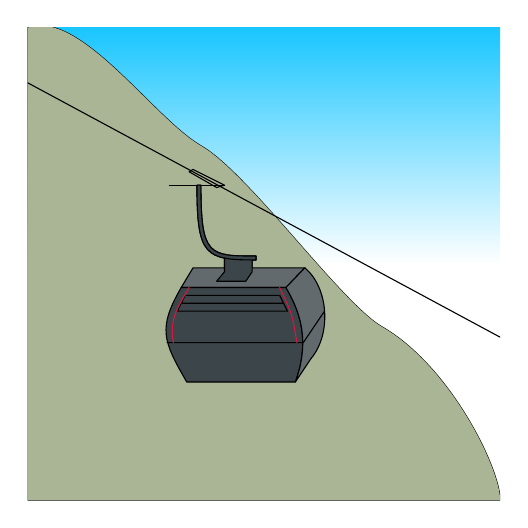
\begin{tikzpicture}[line join=round, line cap=round,scale=1,transform shape]
	\clip (-3,-3) rectangle (3,3);
	\fill[bottom color=white,top color=deepskyblue!90, middle color=white] (-3,-3) rectangle (3,3);
	\tikzset{dat/.pic={
	\def\N{ 
	(-3,3)
	..controls +(20:.7) and +(150:.7) ..(-.8,1.5)
	..controls +(-30:.7) and +(150:.6) ..(1.5,-.8)
	..controls +(-30:1) and +(90:.4) ..(3,-3)--(-3,-3)--cycle
	;
	}
	\draw[black]\N;
	\fill[darkolivegreen!50] \N;
	}}
	\tikzset{cap_treo/.pic={
	\def\X{ 
	(-.85,1)--(-.8,1)
	..controls +(-90:.9) and +(-180:.6) ..(-.1,0.1)--(-.1,.05)
	..controls +(-180:.65) and +(-90:.9) ..cycle
	(-.15,0.05)--(-.15,-.1)--(-.23,-.22)--(-.6,-.22)--(-.5,-.1)--(-.5,.08)
	;
	}
	%\fill[black] \X;
	\draw\X;
	\draw(-3,2.3)--(3.5,-1.2);
	\draw(-1.2,1)--(-.5,1);
	\draw(-.5,1)--(-.9,1.2)--(-.95,1.17)--(-.6,.97)--cycle;
	\draw[fill=arsenic!80](-.9,-.05)--(.52,-.05)--(.28,-.3)--(-1.05,-.3)--cycle;
	\def\M{ 
	(-.85,1)--(-.8,1)
	..controls +(-90:.9) and +(-180:.6) ..(-.1,0.1)--(-.1,.05)
	..controls +(-180:.65) and +(-90:.9) ..cycle
	(-.15,0.05)--(-.15,-.1)--(-.23,-.22)--(-.6,-.22)--(-.5,-.1)--(-.5,.08)
	;
	}
	\fill[arsenic] \M;
	\draw\M;
	\def\N{ 
	(-1.05,-.3)
	..controls +(-120:.6) and +(120:.6) ..(-.98,-1.5)--(.4,-1.5)
	..controls +(70:.6) and +(-60:.3) ..(.28,-.3)--cycle
	;
	}
	\fill[arsenic] \N;
	\draw\N;
	\def\P{ 
	(.4,-1.5)
	..controls +(70:.6) and +(-60:.3) ..(.28,-.3)--(.52,-.05)
	..controls +(-40:.4) and +(50:.4) ..(.6,-1.2)--cycle
	;
	}
	\fill[arsenic!80] \P;
	\draw\P;
	\draw (-1.23,-1)--(.5,-1)--(.77,-.6);
	\draw (-1.05,-.5)--(-1,-.4)--(.2,-.4)--(.25,-.5)--cycle
	(.25,-.5)--(.3,-.6)--(.3,-.6)--(-1.1,-.6)--(.-1.05,-.5)--cycle
	;
	\draw[alizarin](.42,-1)..controls +(100:.4) and +(-65:.4) ..(.2,-.3);
	\draw[alizarin](-1.15,-1)..controls +(100:.3) and +(-120:.3) ..(-.95,-.3);
	}}
	\path
	(0,0)pic[scale=1]{dat}(0,0)pic[scale=1]{cap_treo};
	\end{tikzpicture}
	\begin{tikzpicture}[scale=1, font=\footnotesize, line join=round,xscale=.2, line cap=round,>=stealth]
	\def\a{1/16} 
	\def\xmin{-3} \def\xmax{12}
	\def\ymin{-3} \def\ymax{3} 
	\coordinate (O) at (0,0);
	\coordinate (E) at (-10,-3);
	\coordinate (N) at ($(E)!.7!(O)$);
	\coordinate (P) at ($(E)!.2!(O)$);
	\coordinate (D) at ($(E)!.3!(O)$);
	\coordinate (A) at ($(N)+(3,0)$);
	\coordinate (B) at (-14,1);
	\coordinate (M) at ($(A)!.7!(B)$);
	\draw[->] (\xmin,0)--(\xmax,0) node [above right]{$y$};
	\draw[->] (O)--(0,\ymax) node [left]{$z$};
	\draw[->] (O)--(E) node [below right]{$x$};
	\node at (0,0)[above right]{$O$};
	\draw[dashed] (B)--(P)node [right]{$550$} (N)--(A)node [below right]{$A(10;3;0)$}--(3,0);
	\draw(B)node [above]{$B$}--(A);
	\draw[->,red](O)--(-4,.6)node [above right]{$\overrightarrow{u}$};
	\node at (N) [left]{$10$};
	\node at (M) [above]{$M$};
	\node at (P) [left]{$x_B$};
	\draw[fill=black] (3,0) circle (.5pt) node[below]{\footnotesize $3$};
	%	\path (-28,0) node[opacity=.5,scale=.5] {\includegraphics{image/h35}};
	\clip (\xmin+0.1,\ymin+0.1) rectangle (\xmax-0.1,\ymax-0.1);
	\end{tikzpicture}
	\end{center}
	\choiceTF
	{Phương trình chính tắc của đường cáp là $\dfrac{x+10}{2}=\dfrac{y+3}{-2}=\dfrac{z}{1}$}
	{\True Giả sử sau $t$ (s) kể từ lúc xuất phát $(t \geq 0)$, cabin đến điểm $M$. Khi đó điểm $M$ có tọạ độ là $\left(3 t+10 ;-3 t+3 ;\dfrac{3t}{2}\right)$}
	{Cabin dừng ở điểm $B$ có hoành độ $x_B=550$. Khi đó $AB=750$ m}
	{\True Đường cáp $AB$ tạo với mặt phẳng $(Oxy)$ góc $19^\circ$ (kết quả làm tròn đến hàng đơn vị của độ)}
	\loigiai{
	\begin{itemchoice}
	\itemch Phương trình chính tắc của đường cáp là $\dfrac{x-10}{2}=\dfrac{y-3}{-2}=\dfrac{z}{1}$.
	\itemch Do tốc độ chuyển động của cabin là $4{,}5$ m/s nên độ dài $A M$ bằng $4{,}5 t$ m. \\
	Vì vậy $\left|\overrightarrow{AM}\right|=4{,}5 t$ $(t \geq 0)$.\\
	Do hai véc-tơ $\overrightarrow{A M}$ và $\overrightarrow{u}$ là cùng phương và cùng hướng nên $\overrightarrow{A M}=k \overrightarrow{u}$ với $k$ là số thực dương nào đó. \\
	Suy ra $\left|\overrightarrow{A M}\right|=k|\overrightarrow{u}|=k \cdot \sqrt{2^2+(-2)^2+1}=3 k$. Do đó $3 k=4{,}5 t$. Suy ra $k=\dfrac{3 t}{2}$. \\
	Vì thế, ta có $\overrightarrow{A M}=\dfrac{3 t}{2} \overrightarrow{u}=\left(3 t ;-3 t ; \dfrac{3 t}{2}\right)$.\\
	Gọi tọa độ của điểm $M$ là $\left(x_M ; y_M ; z_M\right)$.\\
	Ta có $\overrightarrow{A M}=\left(x_M-x_A ; y_M-y_A ; z_M-z_A\right)=\left(3 t ;-3 t ; \dfrac{3 t}{2}\right)$.\\
	Nên $\heva{&x_M=3 t+x_A \\ &y_M=-3 t+y_A \\ &z_M=\dfrac{3 t}{2}+z_A}\Leftrightarrow\heva{&x_M=3 t+10 \\ &y_M=-3 t+3 \\ &z_M=\dfrac{3 t}{2}.}$\\
	Vậy điểm $M$ có tọạ độ là $\left(3 t+10 ;-3 t+3 ;\dfrac{3 t}{2}\right)$.
	\itemch Do $x_B=550$ nên $3 t+10=550$, tức là $t=180$ s. Do đó, ta có điểm $B(550 ;-537 ; 270)$. \\
	Vậy $A B=\sqrt{(550-10)^2+(-537-3)^2+(270-0)^2}=\sqrt{656100}=810$ m.
	\itemch Đường thẳng $AB$ có véc-tơ chỉ phương $\overrightarrow{u}=(2 ;-2 ; 1)$ và mặt phẳng $(Oxy)$ có véc-tơ pháp tuyến $\overrightarrow{k}=(0 ; 0 ; 1)$. Do đó, ta có
	$$
	\sin (\Delta,(O x y))=|\cos (\overrightarrow{u},\overrightarrow{k})|=\dfrac{\left|\overrightarrow{u} \cdot \overrightarrow{k}\right|}{|\overrightarrow{u}| \cdot|\overrightarrow{k}|}=\dfrac{1}{3 \cdot 1}=\dfrac{1}{3}.$$
	Vậy $(\Delta,(O x y)) \approx 19^{\circ}$.
	\end{itemchoice}
	}
\end{ex}
\begin{ex}%[Nguyễn Tuấn, dự án sáng tác đề 12 theo chủ đề]%[2H5V2-7]
	Cho hình lăng trụ đứng $OBC.O'B'C'$ có đáy là tam giác $OBC$ vuông tại $O$ và có $OB=3a$, $OC=a$, $OO'=2a$.
	\choiceTF
	{\True Cosin góc giữa hai đường thẳng $BO'$ và $B'C$ bằng $\dfrac{3}{\sqrt{14}}$}
	{\True Cosin góc giữa hai mặt phẳng $(O'BC)$ và $(OBC)$ bằng $\dfrac{6}{7}$}
	{Cosin góc giữa đường thẳng $B'C$ và mặt phẳng $(O'BC)$ bằng $\dfrac{3\sqrt{14}}{49}$}
	{\True Sin góc giữa đường thẳng $B'C$ và mặt phẳng $(O'BC)$ bằng $\dfrac{3\sqrt{14}}{49}$}
	\loigiai
	{
	Xét hệ trục tọa độ $Oxyz$ sao cho các điểm có tọa độ như sau: $O(0;0;0)$, $O'(2a;0;0)$, $B(0;3a;0)$, $C(0;0;1a)$.\\
	Trong không gian $Oxyz$ vừa chọn, ta có $B'(2a;3a;0)$, $C'(2a;0;1a)$, $\overrightarrow{BO}'=(0;-3a;0)$, $\overrightarrow{CB}'=(2a;3a;-a)$.
	\begin{center}
	\begin{tikzpicture}[line cap=round,line join=round,scale=.8,>=stealth,font=\footnotesize ]
	\coordinate (O) at (0,0);
	\coordinate (O') at (0,4.5);
	\coordinate (B) at (5.5,0);
	\coordinate (C) at (2,-2);
	\coordinate (C') at ($(C)+(0,4.5)$);
	\coordinate (B') at ($(B)+(0,4.5)$);
	\coordinate (y) at ($(O)!1.3!(B)$);
	\coordinate (x) at ($(O)!1.3!(O')$);%trung điểm
	\coordinate (z) at ($(O)!1.5!(C)$);%trung điểm
	\draw (B')--(C)--(O')--(B')--(C')--(C)--(B)--(B')(B)--(C')--(O')--(O)--(C)(O)--(C');
	\draw[dashed](O)--(B)--(O');
	\foreach \x/\g in {O'/180,B'/75,C'/180,O/180,B/-80,C/-100}
	\fill[black](\x) circle (1pt)
	($(\x)+(\g:3mm)$) node{$\x$};
	\draw[->](B)--(y)node[below]{$y$};
	\draw[->](O')--(x)node[above]{$x$};
	\draw[->](C)--(z)node[below right]{$z$};
	\end{tikzpicture}
	\end{center}
	\begin{itemchoice}
	\itemch Đúng. Hai đường thẳng $BO'$ và $B'C$ có véc-tơ chỉ phương lần lượt là $\overrightarrow{u}=(0;3;0)$, $\overrightarrow{v}=(2;3;-1)$.\\
	Ta có 
	\begin{eqnarray*}
	\cos (BO',B'C)&=&\dfrac{\left |\overrightarrow{u}\cdot\overrightarrow{v} \right |}{\left |\overrightarrow{u} \right |\cdot\left |\overrightarrow{v} \right |}\\&=&\dfrac{\left |0\cdot 2+3\cdot 3+0\cdot (-1) \right |}{\sqrt{3^2}\cdot\sqrt{2^2+3^2+(-1)^2}}=\dfrac{3}{\sqrt{14}}.
	\end{eqnarray*}
	\itemch Đúng. Ta có phương trình mặt phẳng $(O'BC)$ theo đoạn chắn là $\dfrac{x}{2a}+\dfrac{y}{3a}+\dfrac{z}{a}=1$ hay $3x+2y+6z-6a=0$.\\
	Mặt phẳng $(O'BC)$ có véc-tơ pháp tuyến $\overrightarrow{n}=(3;2;6)$, mặt đáy $(OBC)$ có véc-tơ pháp tuyến $\overrightarrow{k}=(0;0;1)$. Gọi $\alpha$ là góc giữa mặt phẳng $(O'BC)$ và mặt đáy.\\
	Ta có $\cos\alpha =\dfrac{\left |\overrightarrow{n}\cdot\overrightarrow{k} \right |}{\left |\overrightarrow{n} \right |\cdot\left |\overrightarrow{k} \right |}=\dfrac{\left |3\cdot 0+2\cdot 0+6\cdot 1 \right |}{\sqrt{3^2+2^2+6^2}\cdot\sqrt{1^2}}=\dfrac{6}{7}$.
	\itemch Sai. Gọi $\beta$ là góc giữa đường thẳng $B'C$ và mặt phẳng $(O'BC)$.\\
	Ta có $\sin\beta =\dfrac{\left |\overrightarrow{v}\cdot\overrightarrow{n} \right |}{\left |\overrightarrow{v} \right |\cdot\left |\overrightarrow{n} \right |}=\dfrac{\left |2\cdot 3+3\cdot 2+(-1)\cdot 6 \right |}{\sqrt{2^2+3^2+(-1)^2}\cdot\sqrt{3^2+2^2+6^2}}=\dfrac{3\sqrt{14}}{49}$.
	\itemch Đúng. Gọi $\beta$ là góc giữa đường thẳng $B'C$ và mặt phẳng $(O'BC)$.\\
	Ta có $\sin\beta =\dfrac{\left |\overrightarrow{v}\cdot\overrightarrow{n} \right |}{\left |\overrightarrow{v} \right |\cdot\left |\overrightarrow{n} \right |}=\dfrac{\left |2\cdot 3+3\cdot 2+(-1)\cdot 6 \right |}{\sqrt{2^2+3^2+(-1)^2}\cdot\sqrt{3^2+2^2+6^2}}=\dfrac{3\sqrt{14}}{49}$.
	\end{itemchoice}
	}
\end{ex}
\Closesolutionfile{ans}
%\indapan{3}{ans/ans-2-B16-De2-DS}
\Opensolutionfile{ans}[ans/ans-2-B16-De2-KQ]
\caukq
\begin{ex}%[Nguyễn Tuấn, dự án sáng tác đề 12 theo chủ đề]%[2H5H2-7]
	Tính góc giữa hai mặt phẳng $(P_1)\colon x+y+2z-1=0$ và $(P_2)\colon 2x-y+z-2=0$ (đơn vị độ).
	\par\shortans{$60$}
	\loigiai{
	$(P_1)$ có véc-tơ pháp tuyến $\overrightarrow{n}_1=(1;1;2)$;\\
	$(P_2)$ có véc-tơ pháp tuyến $\overrightarrow{n}_2=(2;-1;1)$.\\
	Ta có $\cos((P_1),(P_2))=\dfrac{|\overrightarrow{n}_1\cdot\overrightarrow{n}_2|}{|\overrightarrow{n}_1|\cdot|\overrightarrow{n}_2|}=\dfrac{|1\cdot 2+1\cdot(-1)+2\cdot 1|}{\sqrt{1^2+1^2+2^2}\cdot\sqrt{2^2+(-1)^2+1^2}}=\dfrac{1}{2}$.\\
	$\Rightarrow((P_1),(P_2))=60^{\circ}$.
	}
\end{ex}
\begin{ex}%[Nguyễn Tuấn, dự án sáng tác đề 12 theo chủ đề]%[2H5H2-7]
	Cho mặt phẳng $(P)$ có véc-tơ pháp tuyến $\overrightarrow{n}=(1 ; 2 ; 2)$ và đường thẳng $\Delta$ có véc-tơ chỉ phương $\overrightarrow{u}=(2 ; 2 ;-1)$. Góc giữa đường thẳng $\Delta$ và mặt phẳng $(P)$ bằng bao nhiêu độ (làm tròn kết quả đến hàng đơn vị)?
	\par\shortans{$26$}
	\loigiai{
	Ta có $\sin (\Delta,(P))=\dfrac{|1 \cdot 2+2 \cdot 2+2 \cdot(-1)|}{\sqrt{1^2+2^2+2^2} \cdot \sqrt{2^2+2^2+(-1)^2}}=\dfrac{4}{9}$. \\
	Suy ra $(\Delta,(P)) \approx 26^{\circ}$.
	}
\end{ex}
\begin{ex}%[Nguyễn Tuấn, dự án sáng tác đề 12 theo chủ đề]%[2H5V2-7]
	\immini{
	Trong không gian với hệ tọa độ $Oxyz$, cho hình lăng trụ đứng $OBC.O'B'C'$ với $O(0;0;0)$, $B(2a;0;0)$, $C(0;a;0)$, $O'(0;0;3a)$, $a>0$. Tính sin của góc giữa đường thẳng $B'C$ và mặt phẳng $\left(O'B C\right)$ (kết quả làm tròn đến hàng phần trăm).
	\par\shortans{$0{,}23$}
	}
	{
	\begin{tikzpicture}[scale=.7, font=\footnotesize, line join=round, line cap=round,>=stealth]
	\def\a{1/16} 
	\def\xmin{0} \def\xmax{4}
	\def\ymin{-3} \def\ymax{4.5} 
	\def\h{3}
	\coordinate (O) at (0,0);
	\coordinate (E) at (-2,-3);
	\coordinate (O') at (0,\h);
	\coordinate (B) at ($(E)!.2!(O)$);
	\coordinate (C) at (3,0);
	\coordinate (C') at ($(C)+(0,\h)$);
	\coordinate (B') at ($(B)+(0,\h)$);
	\draw[->] (C)--(\xmax,0) node [above right]{$y$};
	\draw[->] (O')--(0,\ymax) node [left]{$z$};
	\draw[->] (B)node [below right]{$2a$}--(E) node [below right]{$x$};
	\draw[dashed] (O)--(B)--(O')--(C)--cycle (O)--(O');
	\draw (B')--(O')--(C') (B)--(B')--(C')--(C)--cycle (B')--(C);
	\foreach \x/\g in {O/180,B/180,C/45,O'/150,B'/180,C'/45}
	\fill[black] 	(\x) circle (1pt)
	($(\g:4mm)+(\x)$) node {$\x$};	
	\clip (\xmin+0.1,\ymin+0.1) rectangle (\xmax-0.1,\ymax-0.1);
	\node at (C) [below]{$a$};
	\node at (O') [above right]{$3a$};
	\end{tikzpicture}
	}
	\loigiai{
	\begin{itemize}
	\item Ta có $\overrightarrow{BB'}=\overrightarrow{O O'}=(0 ; 0 ; 3 a)$. \\
	Suy ra $x_{B'}=x_B=2a$, $y_{B'}=y_B=0$, $z_{B'}-0=3 a$, tức là $B'(2a;0;3a)$.
	\item Vì $B(2a;0;0)$, $C(0;a;0)$, $O'(0;0;3a)$ nên mặt phẳng $\left(O' B C\right)$ có phương trình là
	\[\dfrac{x}{2a}+\dfrac{y}{a}+\dfrac{z}{3a}=1 \Leftrightarrow 3 x+6 y+2 z-6 a=0.\]
	\item Mặt phẳng $\left(O'B C\right)$ có một véc-tơ pháp tuyến là $\overrightarrow{n}=(3;6;2)$.\\
	Do $B'(2a;0;3a)$, $C(0;a;0)$ nên $\overrightarrow{B'C}=(-2 a;a;-3a)$, suy ra véc-tơ $\overrightarrow{B'C}=(-2 a ; a ;-3 a)$ cùng phương với véc-tơ $\overrightarrow{u}=(-2 ; 1 ;-3)$. \\
	Vì thế véc-tơ $\overrightarrow{u}=(-2 ; 1 ;-3)$ là một véc-tơ chỉ phương của đường thẳng $B'C$. \\
	Suy ra sin của góc giữa đường thẳng $B'C$ và mặt phẳng $\left(O'B C\right)$ bằng
	\[\dfrac{|3 \cdot(-2)+6 \cdot 1+2 \cdot(-3)|}{\sqrt{3^2+6^2+2^2} \cdot \sqrt{(-2)^2+1^2+(-3)^2}}=\dfrac{6}{7 \sqrt{14}}=\dfrac{3 \sqrt{14}}{49}\approx 0{,}23.\]
	\end{itemize}
	}
\end{ex}
\begin{ex}%[Nguyễn Tuấn, dự án sáng tác đề 12 theo chủ đề]%[2H5V2-7]
	\immini{
	Trên một sườn núi (có độ nghiêng đều), người ta trồng một cây thông và muốn giữ nó không bị nghiêng bằng hai sợi dây neo như Hình bên. Giả thiết cây thông mọc thẳng đứng và trong một hệ tọa độ phù hợp, các điểm $O$ (gốc cây thông) và $A, B$ (nơi buộc dây neo) có tọa độ tương ứng là $O(0 ; 0 ; 0)$, $A(3 ;-4 ; 2)$, $B(-5 ;-2 ; 1)$, đơn vị trên mỗi trục tọa độ là mét (Hình bên). Biết rằng hai dây neo đều được buộc vào cây thông tại điểm $(0 ; 0 ; 5)$ và được kéo căng tạo thành các đoạn thẳng.
	}
	{
	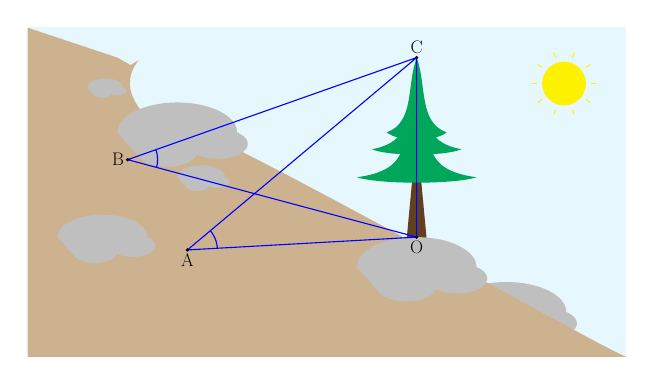
\begin{tikzpicture}[scale=0.38,transform shape,font=\LARGE]
	\draw[draw=none] (0,0)rectangle(20,11);
	\clip (0,0)rectangle(20,11);
	\fill[cyan!10](0,0)rectangle(27,15);
	\tikzset{Icon-mattroi/.pic={
	\def\r{0.35}
	\fill[opacity=1](0,0)circle(\r);
	\draw[line width=2*\r pt](0,0)circle(\r);
	\foreach \g in{1,...,10}{
	\draw[line width=\r pt](\g*36:1.2*\r)++(\g*36:0.1*\r)--++(\g*36:\r*0.25);
	}
	}}
	\tikzset{Doi-Oxyz/.pic={
	\fill[brown!90!teal!60](0,0)--(0,11)--(3,10)--++(-30:0.5)..controls++(-150:-1)and++(135:2)..(4,8)--++(20:0.25)..controls++(60:0.6) and++(160:1)..(20,0)--cycle;
	}}
	\tikzset{da/.pic={
	\fill[gray!50!white](0,0)arc(180:0: 2 and 1)arc(50:-135: 1 and 0.5)arc(-10:-150: 1 and 0.5);
	}}
	\tikzset{cay/.pic={
	\fill[brown!50!black](-0.75,-8)--(0.75,-8)--(0,0)--cycle;
	\fill[green!30!teal][xscale=2,yscale=0.75,shift={(0,-4)}](-2,0)..controls++(-40:1) and++(-140:1)..(2,0)..controls++(160:2)and++(-70:2)..(0,5)..controls++(-110:2)and++(20:2)..(-2,0);
	\fill[green!30!teal][xscale=1.5,yscale=0.75,shift={(0,-1.5)}](-2,0)..controls++(-40:1) and++(-140:1)..(2,0)..controls++(160:2)and++(-70:2)..(0,5)..controls++(-110:2)and++(20:2)..(-2,0);
	\fill[green!30!teal](-2,0)..controls++(-40:1) and++(-140:1)..(2,0)..controls++(160:2)and++(-70:2)..(0,5)..controls++(-110:2)and++(20:2)..(-2,0);
	}}
	\path(14,1.5)pic{da};
	\path(0,0)pic{Doi-Oxyz}(13,7.5)pic[scale=0.5]{cay};
	\foreach \x/\y/\sca in {1/4/0.75,11/3/1,5/6/0.4,3/7.5/1,2/9/0.3}
	\path(\x,\y)pic[scale=\sca]{da};
	\draw[blue](13,10)coordinate(C)--++(220:10)coordinate(A)--(13,4)coordinate(O)--cycle (O)--++(165:10)coordinate(B)--(C);
	\foreach \d in{O,A,B,C}
	\draw[fill=blue](\d)circle(1pt);
	\begin{scope}
	\clip(O)--(A)--(C)--cycle;
	\draw[blue](A)circle(1 cm);
	\end{scope}
	\begin{scope}
	\clip(O)--(B)--(C)--cycle;
	\draw[blue](B)circle(1 cm);
	\end{scope}
	\path(O)node[below]{O}(A)node[below]{A}(B)node[left]{B}(C)node[above]{C}(C)++(-10:5)pic[yellow,scale=2]{Icon-mattroi};
	\end{tikzpicture}
	}
	\noindent Tính tổng số đó các góc tạo bởi mỗi dây neo và mặt phẳng sườn núi (làm tròn kết quả đến hàng đơn vị của độ).
	\par\shortans{$92$}
	\loigiai{
	Ta có $\overrightarrow{O A}=(3 ;-4 ; 2), \overrightarrow{O B}=(-5 ;-2 ; 1)$ nên
	$$
	\left[\overrightarrow{OA}, \overrightarrow{O B}\right]=\left(\left|\begin{array}{ll}
	-4 & 2 \\
	-2 & 1
	\end{array}\right| ;\left|\begin{array}{cc}
	2 & 3 \\
	1 & -5
	\end{array}\right| ; \left| \begin{array}{cc}
	3 & -4 \\
	-5 & -2
	\end{array}\right|\right)=(0 ;-13 ;-26).
	$$
	Vì thế, véc-tơ $\overrightarrow{n}=(0 ; 1 ; 2)$ là một véc-tơ pháp tuyến của mặt phẳng $(O A B)$.\\
	Mặt khác, do $\overrightarrow{C A}=(3 ;-4 ;-3)$, $\overrightarrow{B C}=(5 ; 2 ; 4)$ nên ta có
	\[\sin (C A,(O A B))=|\cos (\overrightarrow{CA}, \overrightarrow{n})|=\dfrac{|\overrightarrow{C A} \cdot \overrightarrow{n}|}{|\overrightarrow{C A}| \cdot|\overrightarrow{n}|}=\dfrac{|3 \cdot 0+(-4) \cdot 1+(-3) \cdot 2|}{\sqrt{34} \cdot \sqrt{5}}=\dfrac{10}{\sqrt{170}}.\]
	Suy ra $(C A,(O A B)) \approx 50^{\circ}$. Vậy góc tạo bởi dây neo $C A$ và mặt phẳng sườn núi là khoảng $50^{\circ}$.\\
	Lại có
	$$
	\sin (B C,(O A B))=|\cos (\overrightarrow{B C}, \overrightarrow{n})|=\dfrac{|\overrightarrow{B C} \cdot \overrightarrow{n}|}{|\overrightarrow{B C}| \cdot|\overrightarrow{n}|}=\dfrac{|5 \cdot 0+2 \cdot 1+4 \cdot 2|}{3 \sqrt{5} \cdot \sqrt{5}}=\dfrac{2}{3},
	$$
	suy ra $(B C,(O A B)) \approx 42^{\circ}$. \\
	Vậy góc tạo bởi dây neo $B C$ và mặt phẳng sườn núi là khoảng $42^{\circ}$.\\
	Vậy tổng số đo $2$ góc là $92^\circ$.
	}
\end{ex}
\begin{ex}%[Nguyễn Tuấn, dự án sáng tác đề 12 theo chủ đề]%[2H5V2-7]
	\immini{	Trong không gian với hệ tọa độ $Oxyz$, cho hình chóp $S.ABCD$ có các đỉnh lần lượt là $S\left(0;0;\dfrac{a\sqrt{3}}{2}\right)$, $A\left(\dfrac{a}{2};0;0\right)$, $B\left(-\dfrac{a}{2};0;0\right)$, $C\left(-\dfrac{a}{2};a;0\right)$, $D\left(\dfrac{a}{2};a;0\right)$ với $a>0$. Tính góc giữa đường thẳng $SD$ và mặt phẳng $(SAC)$ (làm tròn kết quả đến hàng đơn vị của độ).
	\shortans{$28$}
	}{\begin{tikzpicture}[scale=0.6, font=\footnotesize,line join=round, line cap=round, >=stealth]
	\coordinate (B) at (0,0);
	\coordinate (A) at (-2,-2);
	\coordinate (J) at ($(A)!0.5!(B)$);
	\coordinate (x) at ($(B)!1.2!(A)$);
	\coordinate (C) at (5,0);
	\coordinate (D) at ($(A)+(C)-(B)$);
	\coordinate (I) at ($(C)!0.5!(D)$);
	\coordinate (y) at ($(J)!1.2!(I)$);
	\coordinate (S) at ($(J)+(0,4)$);
	\coordinate (z) at ($(J)!1.2!(S)$);
	\draw[dashed] (S)--(J)--(I);
	\draw[->](S)--(z) node[above]{$z$};
	\draw[->](I)--(y) node[below]{$y$};
	\draw[->](A)--(x) node[below,left]{$x$};
	\draw (S)--(C)--(D)--(A)--(S)--(D);
	\draw[dashed,thin] (C)--(B)--(A)--(D) (S)--(B);
	\draw (J) node[left]{$O$};
	\foreach \i/\g in {S/180,A/-90,B/-90,C/-90,D/-90}{\draw[fill=black](\i) circle (1.5pt) ($(\i)+(\g:3mm)$) node[scale=1]{$\i$};}
	\end{tikzpicture}}
	\loigiai{
	Ta có $\overrightarrow{SA}=\left(\dfrac{a}{2};0;-\dfrac{\sqrt{3}}{2}\right)$, $\overrightarrow{SC}=\left(-\dfrac{a}{2};a;-\dfrac{a\sqrt{3}}{2}\right)$, 	$\overrightarrow{SD}=\left(\dfrac{a}{2};a;-\dfrac{\sqrt{3}}{2}\right)$.\\
	$\left[\overrightarrow{SA};\overrightarrow{SC}\right]=\left(\dfrac{a^2\sqrt{3}}{2};\dfrac{a^2\sqrt{3}}{2};\dfrac{a^2}{2}\right)=\dfrac{a^2}{2}\cdot \overrightarrow{n}$, với $\overrightarrow{n}=(\sqrt{3};\sqrt{3};1)$.\\
	Ta có\\
	$\sin(SD,(SAC))=\dfrac{|\overrightarrow{n}\cdot\overrightarrow{SD}|}{|\overrightarrow{n}|\cdot|\overrightarrow{SD}|}=\dfrac{\left|\dfrac{a\sqrt{3}}{2}+a\sqrt{3}-\dfrac{a\sqrt{3}}{2}\right|}{\sqrt{(\sqrt{3})^2+(\sqrt{3})^2+1^2}\cdot\sqrt{\left(\dfrac{a}{2}\right)^2+a^2+\left(\dfrac{-a\sqrt{3}}{2}\right)^2}}=\dfrac{\sqrt{42}}{4}$.\\
	Suy ra $(SD,(SAC))\approx 28^{\circ}$.
	}
\end{ex}
\begin{ex}%[Nguyễn Tuấn, dự án sáng tác đề 12 theo chủ đề]%[2H5V2-7]
	\immini
	{
	Để chuẩn bị cho chuyến đi dã ngoại, nhóm bạn Đức thiết kế lều cắm trại dạng hình chóp tứ giác đều có đáy là hình vuông cạnh $4$m. Theo bản vẽ thiết kế thì góc giữa hai mặt bên của lều bằng $60^{\circ}$. Bằng phương pháp tọa độ, hãy tính chiều cao của lều này (đơn vị: mét).
	\shortans{$2$}
	}
	{
	\begin{tikzpicture}[>=stealth,line join=round,line cap=round,font=\footnotesize,scale=0.9]
	\def \cao{3};
	\def \x{3};
	\coordinate (D) at (0,0);
	\coordinate (C) at (1,.8);
	\coordinate (A) at (\x,0);
	\coordinate (B) at ($(A)-(D)+(C)$);
	\coordinate (O) at ($(C)!.5!(A)$);
	\coordinate (S) at ($(O)+(90:\cao)$);
	\coordinate (X) at (intersection of S--O and D--A);
	\draw (D)--(A)--(B)--(S)--cycle (S)--(A);
	\draw[dashed] (C)--(B) (S)--(C)--(D);
	\draw[dashed,red] (A)--($(A)!1.2!(C)$) (D)--(B) (S)--(X);
	\draw[->,red] (A)--($(O)!1.6!(A)$) node[right]{$x$};
	\draw[->,red] (B)--($(O)!1.4!(B)$) node[above]{$y$};
	\draw[->,red] (S)--($(O)!1.3!(S)$) node[left]{$z$};
	\draw[red] (X)--++(-90:0.7) (D)--($(O)!1.3!(D)$);
	\foreach \diem/\goc in {C/45,D/-90,A/-90,B/-30,S/45,O/-130} \fill[black](\diem) circle (1pt) ($(\diem)+(\goc:3mm)$) node{$\diem$};
	\end{tikzpicture}
	}
	\loigiai{
	Ta có $AC=BD=\sqrt{AD^2+AB^2}=\sqrt{4^2+4^2}=4\sqrt{2}$.\\
	Chọn hệ trục tọa độ $Oxyz$ với gốc tọa độ $O$ là giao điểm của hai đường chéo $AC$ và $BD$ như hình vẽ.\\
	Gọi $z$ là chiều cao của lều.\\
	Ta có $O(0;0;0)$, $A(2\sqrt{2};0;0)$, $B(0;2\sqrt{2};0)$, $C(-2\sqrt{2};0;0)$, $D(0;-2\sqrt{2};0),S(0;0;z)$, với $z>0$.\\
	Ta có $\overrightarrow{AD}=(-2\sqrt{2};-2\sqrt{2};0),\overrightarrow{AB}=(-2\sqrt{2};2\sqrt{2};0),\overrightarrow{AS}=(-2\sqrt{2};0;z)$.\\
	Véc-tơ pháp tuyến của $(SAD)$ là $\overrightarrow{n}_1=\left[\overrightarrow{AD},\overrightarrow{AS}\right]=(-2z\sqrt{2};2z\sqrt{2};-8)$.\\
	Véc-tơ pháp tuyến của $(SAB)$ là $\overrightarrow{n}_2=\left[\overrightarrow{AB},\overrightarrow{AS}\right]=(2z\sqrt{2};2z\sqrt{2};8)$.\\
	Ta có
	\begin{eqnarray*}
	\cos((SAD),(SAB))&=&\dfrac{|\overrightarrow{n}_1\cdot \overrightarrow{n}_2|}{|\overrightarrow{n}_1|\cdot |\overrightarrow{n}_2|}\\
	&=&\dfrac{|-2z\sqrt{2}\cdot 2z\sqrt{2}+2z\sqrt{2}\cdot 2z\sqrt{2}+8\cdot(-8)|}{\sqrt{(-2z\sqrt{2})^2+(2z\sqrt{2})^2+(-8)^2}\cdot \sqrt{(2z\sqrt{2})^2+(2z\sqrt{2})^2+8^2}}\\
	&=&\dfrac{64}{16z^2+64}.
	\end{eqnarray*}
	Vì góc giữa hai mặt bên bằng $60^{\circ}$ nên góc giữa hai mặt phẳng $(SAD)$ và $(SAB)$ bằng $60^{\circ}$.\\
	Do đó
	$$\cos 60^{\circ}=\dfrac{64}{16z^2+64} \Leftrightarrow \dfrac{1}{2}=\dfrac{64}{16z^2+64}\Leftrightarrow 16z^2+64=128\Leftrightarrow \hoac{&z=2\\&z=-2}$$
	Vì $z>0$ nên ta có $S(0;0;2)$.\\
	Vậy chiều cao của lều là $2$ m.
	}
\end{ex}
\Closesolutionfile{ans}
% %\indapan{6}{ans/ans-2-B16-De2-KQ}

\begin{name}
	{\tenchude}
	{TOÁN 12 - PHƯƠNG TRÌNH MẶT CẦU}
	{LỚP TOÁN THẦY PHÁT}
	{Thời gian: 90 phút - Không kể thời gian phát đề}
\end{name}

\Opensolutionfile{ans}[ans/ans-2-B17-De1]
\caulc
\begin{ex}%Cau1
	Trong không gian với hệ trục tọa độ $Oxyz$, phương trình nào sau đây là phương trình mặt cầu
	\choice
	{\True $x^2+y^2+z^2-2x=0$}
	{$x^2+y^2-z^2+2x-y+1=0$}
	{$2x^2+2y^2=\left( x+y \right)^{2}-z^2+2x-1 $}
	{$\left(x+y \right)^{2}=2xy-z^2-1 $}
	\loigiai{Phương trình mặt cầu $\left(S \right)$ có hai dạng là:
\begin{description}
\item[{\rm (1)}] $\left(x-a \right)^2+\left(y-b \right)^2+\left(z-c \right)^2=R^2$
\item[{\rm (2)}] $x^2+y^2+z^2-2ax-2by-2cz+d=0 \text{ với } a^2+b^2+c^2-d>0$
\end{description}	
$\ast$ $x^2+y^2+z^2-2x=0$ là phương trình mặt cầu.\\
$\ast$ $x^2+y^2-z^2+2x-y+1=0$ không là phương trình mặt cầu.\\
$\ast$ $2x^2+2y^2=\left( x+y \right)^{2}-z^2+2x-1 \Leftrightarrow x^2+y^2+z^2-2xy-2x+1=0$ không là phương trình mặt cầu.\\
$\ast$ $\left(x+y \right)^{2}=2xy-z^2-1 \Leftrightarrow x^2+y^2+z^2+1=0$ không là phương trình mặt cầu vì $a^2+b^2+c^2-d=-1<0$. 
}
\end{ex}	
\begin{ex}%Cau2
Trong không gian với hệ trục tọa độ $Oxyz$, mặt cầu $\left(S \right) \left( x-1\right)^2+y^2+\left( z+3\right)^2=16$ có tâm là
	\choice
	{$I\left(1;0;3\right)$}
	{$I\left(-1;0;-3\right)$}
	{\True $I\left(1;0;-3\right)$}
	{$I\left(1;2;-3\right)$}
	\loigiai{
	Phương trình mặt cầu $\left( S \right)$ có dạng là:
$\left(x-a \right)^2+\left(y-b \right)^2+\left(z-c \right)^2=R^2$ có tâm $I\left(a;b;c\right)$ bán kính là $R$\\
Khi đó mặt cầu $\left(S\right)$ có tâm $I\left(1;0;-3\right)$.}
\end{ex}
\begin{ex}%Cau3
Trong không gian với hệ trục tọa độ $Oxyz$, mặt cầu $x^2+y^2+z^2-4x+1=0$ có tâm và bán kính là
	\choice
	{$I\left(2;0;0\right)$, $R=3$}
	{$I\left(-2;0;0\right)$, $R=\sqrt{3}$}
	{$I\left(0;2;0\right)$, $R=\sqrt{3}$}
	{\True $I\left(2;0;0\right)$, $R=\sqrt{3}$}
	\loigiai{
	Phương trình mặt cầu $\left( S \right)$ có dạng là:
$x^2+y^2+z^2-2ax-2by-2cz+d=0$ có tâm $I\left(a;b;c\right)$, có bán kính là $R =\sqrt{a^2+b^2+c^2-d}$\\
Khi đó, mặt cầu $x^2+y^2+z^2-4x+1=0$ có tâm là $I\left(2;0;0\right)$, có bán kính là $R=\sqrt{2^2+0^2+0^2-1}=\sqrt{3}$.}
\end{ex}
\begin{ex}%Cau4 
Trong không gian với hệ trục tọa độ $Oxyz$, phương trình mặt cầu có tâm $I\left(-3;1;2\right)$, bán kính $R=3$ là
	\choice
	{$\left(x+3 \right)^2+\left(y-1 \right)^2+\left(z+2 \right)^2=3$}
	{$\left(x-1 \right)^2+\left(y+3 \right)^2+\left(z-2 \right)^2=9$}
	{$\left(x-3 \right)^2+\left(y+1 \right)^2+\left(z+2 \right)^2=9$}
	{\True $\left(x+3 \right)^2+\left(y-1 \right)^2+\left(z-2 \right)^2=9$}
	\loigiai{
	Phương trình mặt cầu có tâm $I\left(-3;1;2\right)$, có bán kính $R=3$ là: $$\left(x+3 \right)^2+\left(y-1 \right)^2+\left(z-2 \right)^2=9$$ }
\end{ex}
\begin{ex}%Cau5
Mặt cầu ${3x}^2+{3y}^2+{3z}^2-6x+12y+2=0$ có bán kính bằng
\choice
	{\True $R=\sqrt{\dfrac{13}{3}}$}
	{$R=\dfrac{\sqrt{7}}{3}$}
	{$R=\dfrac{2\sqrt{7}}{3}$}
	{$R=\dfrac{\sqrt{21}}{3}$}
	\loigiai{
	Biến đổi ${3x}^2+{3y}^2+{3z}^2-6x+12y+2=0 \Leftrightarrow x^2+y^2+z^2-2x+4y+\dfrac{2}{3}=0$ có tâm $I\left(1;-2;0\right)$ và bán kính $R= \sqrt{1^2+\left(-2 \right)^2+0^2-\dfrac{2}{3}}=\sqrt{\dfrac{13}{3}}$.}
\end{ex}
\begin{ex}%Cau6
Mặt cầu $\left(S \right)$ : $x^2+y^2+z^2-2x+10y+3z+1=0$ đi qua điểm có tọa độ nào sau đây
\choice
	{$\left(3;-2;-4 \right) $}
	{\True $\left(4;-1;0 \right) $}
	{$\left(2;1;9 \right) $}
	{$\left(-1;3;-1 \right) $}
	\loigiai{
	Lần lượt thay các tọa độ các điểm vào phương trình mặt cầu. Tọa độ điểm nào thỏa mãn phương trình thì điểm đó thuộc mặt cầu.\\
	$\ast$ Với đáp án $\textbf{A}$, ta thay $x=3,y=-2,z=-4$ vào $\left(S\right)$.\\
	 Ta có $3^2+\left(-2\right)^2+\left(-4\right)^2-2.3+10.\left(-2\right)+3.\left(-4\right)+1=-8\neq0$. Khi đó $\left(3;-2;-4\right) \notin \left(S\right)$ nên ta loại đáp án $\textbf{A}$\\
	$\ast$ Tương tự với đáp án $\textbf{B}$. Ta có $4^2+\left(-1\right)^2+0^2-2.4+10.\left(-1\right)+3.0+1=0$. Khi đó $\left(4;-1;0\right) \in \left(S\right)$ nên ta chọn $\textbf{B}$\\
	$\ast$ Với đáp án $\textbf{C}$. Ta có $2^2+1^2+9^2-2.2+10.1+3.9+1=120$. Khi đó $\left(2;1;9\right) \notin \left(S\right)$ nên ta loại đáp án $\textbf{C}$\\
	$\ast$ Với đáp án $\textbf{D}$. Ta có $\left(-1\right)^2+3^2+\left(-1\right)^2-2.\left(-1\right)+10.3+3.\left(-1\right)+1=41$. Khi đó $\left(-1;3;-1\right) \notin \left(S\right)$ nên ta loại đáp án $\textbf{D}$}
\end{ex}
\begin{ex}%Cau7
Mặt cầu tâm $I\left(-1;2;-3 \right)$ và đi qua điểm $A\left(2;0;0 \right)$ có phương trình là
\choice
	{\True $\left(x+1 \right)^2+\left(y-2 \right)^2+\left(z+3 \right)^2=22$}
	{$\left(x+1 \right)^2+\left(y-2 \right)^2+\left(z+3 \right)^2=11$}
	{$\left(x-1 \right)^2+\left(y+2 \right)^2+\left(z-3 \right)^2=22$}
	{$\left(x-1 \right)^2+\left(y-2 \right)^2+\left(z-3 \right)^2=22$}
	\loigiai{
	Ta có $\vec{IA}=\left( 3;-2;3\right)$, $R=IA=\sqrt{22}$\\
	Vậy phương trình mặt cầu tâm $I\left(-1;2;-3 \right)$, bán kính $R=\sqrt{22}$ là: $$\left(x+1 \right)^2+\left(y-2 \right)^2+\left(z+3 \right)^2=22$$
	}
\end{ex}
\begin{ex}%Cau8
Mặt cầu $\left(S \right):\left(x+y \right)^2=2xy-z^2+1-4x$ có tâm là
\choice
	{$I\left(4;0;0\right)$}
	{\True $I\left(-2;0;0\right)$}
	{$I\left(-4;0;0\right)$}
	{$I\left(2;0;0\right)$}
	\loigiai{
	Ta biến đổi $\left(x+y\right)^2=2xy-z^2+1-4x \Leftrightarrow x^2+y^2+z^2+4x-1=0$\\
	Vậy mặt cầu có tâm $I\left(-2;0;0\right)$.}
\end{ex}
\begin{ex}%Cau9
Trong không gian với hệ trục tọa độ $Oxyz$, cho hai điểm $A\left(1;0;-3 \right)$ và $B\left(3;2;1 \right)$. Phương trình mặt cầu đường kính $AB$ là
\choice
	{$x^2+y^2+z^2+4x-2y+2z=0$}
	{\True $x^2+y^2+z^2-4x-2y+2z=0$}
	{$x^2+y^2+z^2-2x-y+z-6=0$}
	{$x^2+y^2+z^2-4x-2y+2z+6=0$}
	\loigiai{
Ta có $\vec{AB}=\left(2;2;4\right) \Rightarrow AB=2\sqrt{6}$.
	Mặt cầu đường kính $AB$ có tâm $I$ là trung điểm $AB$ nên $I\left(2;1;-1\right)$, bán kính $R=\dfrac{AB}{2}=\sqrt{6}$.\\
	Khi đó phương trình mặt cầu: $\left(x-2\right)^2+\left(y-1\right)^2+\left(z+1\right)^2=6$.\\
	 hay $x^2+y^2+z^2-4x-2y+2z=0$.}
\end{ex}
\begin{ex}%Cau10
Phương trình mặt cầu $\left(S \right)$ có tâm $O$, tiếp xúc với mặt phẳng $\left(\alpha\right):16x-15y-12z+75=0$ là
\choice
	{$x^2+y^2+z^2-3x=9$}
	{$x^2+y^2+z^2=3$}
	{$x^2+y^2+z^2=81$}
	{\True $x^2+y^2+z^2=9$}
	\loigiai{
	Do $\left( S\right)$ tiếp xúc với $\left(\alpha\right)$ nên $\mathrm{d}\left(O;\left( \alpha\right)\right) = R \Leftrightarrow R = \dfrac{75}{25}=3$.\\
	Mặt cầu tâm $O\left( 0;0;0\right)$ và bán kính $R=3$ có phương trình $\left( S\right): x^2+y^2+z^2=9$.}
\end{ex}
\begin{ex}%Cau11
Cho mặt phẳng $\left(P\right)$ và mặt cầu $\left(S\right)$ có phương trình lần lượt là\\
 $\left(P\right): 2x+2y+z-m^2+4m-5=0$ và $\left(S\right): x^2+y^2+z^2-2x+2y-2z-6=0$. Giá trị của $m$ để $\left(P\right)$ tiếp xúc với $\left(S\right)$ là
\choice
	{\True $m=-1$ hoặc $m=5$}
	{$m=1$ hoặc $m=-5$}
	{$m=-1$}
	{$m=5$}
	\loigiai{
	Dễ thấy mặt cầu $\left(S \right)$ có tâm $I\left(1;-1;1\right)$ và bán kính $R=\sqrt{1^2+\left( -1\right)^2+1^2+6}=3$.\\
	Khi $\left(P\right)$ tiếp xúc với $\left(S\right)$ ta có:
\begin{eqnarray*}
& &\mathrm{d}\left(I;\left(P \right)\right)=R\\
&\Leftrightarrow & \dfrac{\vert 2\cdot1+2\cdot\left(-1\right)+1\cdot1-m^2+4m-5 \vert}{\sqrt{2^2+2^2+1^2}}=3\\
&\Leftrightarrow & \vert m^2-4m+4 \vert = 9\\
&\Leftrightarrow & \hoac{&m^2-4m+4=9\\&m^2-4m+4=-9}\\
&\Rightarrow & m^2-4m-5=0\\
&\Rightarrow &\hoac{&m=-1\\&m=5}.
\end{eqnarray*}}
\end{ex}
\begin{ex}%Cau12
Cho bốn điểm $A\left(6;-2;3\right)$,$B\left(0;1;6\right)$,$C\left(2;0;-1 \right)$,$D\left(4;1;0\right)$. Khi đó mặt cầu ngoại tiếp tứ diện $ABCD$ có phương trình là
\choice
	{$x^2+y^2+z^2-2x+y-3z-3=0$}
	{\True $x^2+y^2+z^2-4x+2y-6z-3=0$}
	{$x^2+y^2+z^2+4x-2y+6z-3=0$}
	{$x^2+y^2+z^2+2x-y+3z-3=0$}
	\loigiai{
	Gọi phương trình mặt cầu $\left( S\right)$ có dạng: $x^2+y^2+z^2-2Ax-2By-2Cz+D=0$ với $A^2+B^2+C^2-D>0$, ta có\\
	$\heva{&A\left(6;-2;3\right)\in \left( S\right)\\&B\left(0;1;6\right)\in \left( S\right)\\&C\left(2;0;-1\right)\in \left( S\right)\\&D\left(4;1;0\right)\in \left( S\right)}$ $\Leftrightarrow \heva{&49-12A+4B-6C+D=0\quad(1)\\&37 -2B-12C+D=0\quad(2)\\&5-4A +2C+D=0\quad(3)\\&17-8A-2B +D=0\quad(4)}$\\
	Lấy $\left(1 \right)-\left( 2\right)$;$\left(2 \right)-\left( 3\right)$;$\left(3 \right)-\left( 4\right)$ ta được hệ\\
	$\heva{&-12A+6B+6C=-12\\&4A-2B-14C=-32\\&4A+2B+2C=12} \Leftrightarrow \heva{&A=2\\&B=-1\\&C=3} \Rightarrow D=3$.\\
	Vậy phương trình mặt cầu là: $x^2+y^2+z^2-4x+2y-6z-3=0$.
	\medskip
	Ở bài này máy tính Casio cũng có thể thực hiện giải hệ phương trình bậc nhất bốn ẩn để tìm các hệ số.
	}
\end{ex}
\Closesolutionfile{ans}
% \indapan{6}{ans/ans-2-B17-De1}
\cauds
\Opensolutionfile{ans}[ans/ans-0-B15-DS]
\begin{ex}%Cau1
Cho $\left(S\right): x^2+y^2+z^2-2x-4y+6z-67=0$. Các mệnh đề sau đúng hay sai ?
\choiceTF
	{Mặt cầu $\left( S\right)$ có tâm $I\left(1;2;3\right)$}
	{\True Bán kính mặt cầu $\left( S\right)$ là $R=9$}
	{Cho mặt phẳng $\left(P\right): 2x-2y+z-13=0$. Khi đó $\left( P\right)$ tiếp xúc với $\left(S\right)$}
	{\True Cho đường thẳng $\left(\Delta\right) :\heva{&x=1+t\\&y=2\\&z=-4+7t}$. Khi đó $\left(\Delta\right)$ và $\left(S\right)$ cắt nhau tại hai điểm}
	\loigiai{
	\begin{itemchoice}
	\itemch Sai. Mặt cầu $\left( S\right)$ có tâm $I\left(1;2;-3\right)$.
	\itemch Đúng. Ta có $R=\sqrt{1^2+2^2+\left(-3\right)^2+67}=\sqrt{81}=9$
	\itemch Sai. Vì $\mathrm{d}\left(I,\left(P\right)\right)=\dfrac{\vert 2\cdot1-2\cdot2+\left(-3\right)-13\vert}{\sqrt{2^2+2^2+\left(-1\right)^2}}=6< R=9$. Suy ra $\left(P\right)$ cắt $\left(S\right)$ theo giao tuyến là một đường tròn.
	\itemch Đúng. Tọa độ giao điểm là nghiệm của hệ phương trình\\
	 $\heva{&x=1+t\\&y=2\\&z=-4+7t\\&x^2+y^2+z^2-2x-4y+6z-67=0}\Rightarrow \hoac{&t=0\\&t=1}$.\\
	 Với $t=0$, thay $t=0$ vào $\left(\Delta\right)$ ta được tọa độ $A\left(1;2;-4\right)$\\
	 Với $t=1$, thay $t=1$ vào $\left(\Delta\right)$ ta được tọa độ $B\left(2;2;3\right)$.\\
	 Vậy, $\left(\Delta\right)$ và $\left(S\right)$ cắt nhau tại hai điểm $A$ và $B$.
	\end{itemchoice}
	}
\end{ex}
\begin{ex}%Cau2
	Trong không gian $Oxyz$ cho ba điểm $A\left(1;0;0\right)$ $B\left(0;2;0\right)$ $C\left(0;0;3\right)$ và phương trình mặt cầu $\left(S \right): \left(x-3\right)^2+\left(y+2\right)^2+\left(z-1\right)^2=9$ Các mệnh đề sau đúng hay sai ?
	\choiceTF
	{\True Thể tích của $\left(S\right)$ là $V=36\pi$ }
	{Phương trình mặt cầu nhận $AB$ làm đường kính có tâm là $I \left(\dfrac{1}{2};1;\dfrac{3}{2}\right)$}
	{Gọi $K$ là tâm của $\left( S \right)$, khi đó $\mathrm{d}\left(K;\left(ABC\right)\right)=\dfrac{9}{7}$ }
	{Tập hợp các điểm $M$ thỏa mãn $MA^2=MB^2+MC^2$ là mặt cầu có bán kính bằng 2}
	\loigiai{
	\begin{itemchoice}
	\itemch Đúng. Với $R=3$. Thể tích của khối cầu $V = \dfrac{4}{3}\pi R^3=\dfrac{4}{3}\pi 3^3=36\pi$
	\itemch Sai. Phương trình mặt cầu nhận trung điểm $I$ của $AB$ làm tâm. Khi đó $I\left(\dfrac{1}{2};1;0\right)$
	\itemch Sai. Ta có $K\left(3;-2;1\right)$\\
	và phương trình mặt phẳng $\left(ABC\right): \dfrac{x}{1}+\dfrac{y}{2}+\dfrac{z}{3}=1$.\\
	Khi đó, $\mathrm{d}\left(K;\left(ABC\right)\right)=\dfrac{\left\vert \dfrac{3}{1}+\dfrac{-2}{2}+\dfrac{1}{3}-1\right\vert}{\sqrt{\left(\dfrac{1}{1}\right)^2+\left(\dfrac{1}{2}\right)^2+\left(\dfrac{1}{3}\right)^2}}=\dfrac{8}{7}$.
	\itemch Sai. Giả sử $M \left(x;y;z\right)$\\
	Ta có $MA^2=\left(x-1\right)^2+y^2+z^2$; $MB^2=x^2+\left(y-2\right)^2+z^2$; $MC^2=x^2+y^2+\left(z-3\right)^2$.\\
	Khi đó, $MA^2=MB^2+MC^2$ \\
	$ \Leftrightarrow \left(x-1\right)^2+y^2+z^2= x^2+\left(y-2\right)^2+z^2 +x^2+y^2+\left(z-3\right)^2 $ \\
	$\Leftrightarrow -2x+1 = \left( y-2 \right)^2+x^2+\left( y-3\right)^2$\\
	 $\Leftrightarrow \left(x+1\right)^2+\left(y-2\right)^2+\left(z-3\right)^2=2$\\
	Vậy tập hợp các điểm $M$ là mặt cầu có bán kính là $R= \sqrt{2}$.
	\end{itemchoice}
	}
\end{ex}
\begin{ex}%Cau3
	Trong không gian với hệ trục tọa độ $Oxyz$ cho mặt phẳng $\left(P\right): 2x+2y-z+16=0$ và mặt cầu $\left(S\right): \left(x-2\right)^2+\left(y-1\right)^2+\left(z-3\right)^2=9$. Các khẳng định nào dưới đây đúng hay sai ?
	\choiceTF
	{Khoảng cách từ tâm $I$ của $\left(S\right)$ đến mặt phẳng $\left(P\right)$ bằng 3 }
	{\True $\left(P\right)$ và $\left(S\right)$ không có điểm chung }
	{Cho mặt phẳng $\left(Q\right):3x-2y+z-10=0$, khi đó $\left(S\right)$ cắt $\left(Q\right)$ theo một giao tuyến là đường tròn có chu vi bằng $\dfrac{3\sqrt{182}}{14} \pi$}
	{\True Cho điểm $M$ di động trên $\left(S\right)$ và điểm $\left(N\right)$ di động trên $\left(P\right)$ sao cho độ dài $MN$ ngắn nhất. Tọa độ điểm $M$ là $M\left(0;-3;4\right)$}
	\loigiai{
	\begin{itemchoice}
	\itemch Sai. Ta có mặt cầu tâm $I\left(2;-1;3\right)$ và có $R=3$. Khoảng cách từ $I$ đến $\left(P\right)$ là\\
	$\mathrm{d}\left(I,\left(P\right)\right)=\dfrac{ \left\vert 2\cdot2+2\cdot\left(-1\right)-3+16 \right\vert}{3}=5$. 
	\itemch Đúng. Vì $\mathrm{d}\left(I,\left(P\right)\right)=5>R=3$ nên $\left(P\right)$ và $\left(S\right)$ không có điểm chung.
	\itemch Sai. Ta có $\mathrm{d}=\mathrm{d}\left(I,\left(Q\right)\right)=\dfrac{3\sqrt{14}}{14}$.\\
	Gọi $r$ là bán kính của đường tròn giao tuyến của $\left(S\right)$ cắt $\left(Q\right)$. \\
	Khi đó $r=\sqrt{R^2-d^2}= \dfrac{3\sqrt{182}}{14}$. Khi đó chu vi cần tìm là $C=2\pi r= \dfrac{3\sqrt{182}}{7} \pi$
	\itemch Đúng. Do $\left(P\right)$ và $\left(S\right)$ không có điểm chung nên $MN_{min}=d-R=2$;\\
	Khi đó $N$ là hình chiếu vuông góc của $I$ lên mặt phẳng $\left(P\right)$ và $M$ là giao điểm của đoạn thẳng $IN$ với mặt cầu $\left(S\right)$\\
	Gọi $\left(d\right)$ là đường thẳng đi qua điểm $I$ và vuông góc với $\left(P\right)$, thì $\left(d\right) \cap \left(P\right) = N$\\
	và $\overrightarrow{u}_{\left(d\right)}=\overrightarrow{u}_{\left(P\right)}=\left(2;2;-1\right)$. Phương trình đường thẳng $\left(d\right): \heva{&x=2+2t\\&y=-1+2t\\&z=3-t}$\\
	$N\in \left(d\right) \Rightarrow N\left(2+2t;-1+2t;3-t\right)$ mà $N \in \left(P\right)$\\
	$\Rightarrow 2\left(2+2t\right)+2\left(-1+2t\right)-\left(3-t\right)+16=0 \Leftrightarrow 9t+15=0 \Leftrightarrow t=\dfrac{-5}{3}$ \\
	Suy ra $N\left(-\dfrac{4}{3};-\dfrac{13}{3};\dfrac{14}{3}\right)$. Ta có $\overrightarrow{IM}=\dfrac{3}{5} \overrightarrow{IN} \Rightarrow M \left(0;-3;4 \right)$.
	\end{itemchoice}
	}
\end{ex}
\begin{ex}%Cau4
	Cho mặt cầu $\left(S\right): x^2+y^2+z^2-2x-4y-6z-m=0$.
	\choiceTF
	{Điều kiện của $m$ để mặt cầu $\left(S\right)$ xác định là $m>14 $}
	{\True Với $m=2$, đường tròn giao tuyến của $\left(S\right)$ khi cắt mặt phẳng $\left(Oxy\right)$ có chu vi bằng $2\sqrt{7}\pi$ }
	{Với $m=2$, Phương trình mặt cầu đối xứng với mặt cầu $\left(S\right)$ qua trục $Oz$ có phương trình $\left(x+1\right)^2+\left(y+2\right)^2+\left(z+3\right)^2=16$}
	{\True Với $m=2$, cho mặt phẳng $\left(P\right): x+y-2x+4=0$. Phương trình đường thẳng $d$ tiếp xúc với $\left(S\right)$ tại $A\left(-1;0;0\right)$ và song song với mặt phẳng $\left(P\right)$ là $\heva{&x=-1+7t\\&y=-7t\\&z=0}$ }
	\loigiai{
	\begin{itemchoice}
	\itemch Sai. Phương trình mặt cầu $\left(S\right): x^2+y^2+z^2-2ax-2by-2cz+d=0$ xác định khi $a^2+b^2+c^2-d>0 \Leftrightarrow 14+m>0 \Leftrightarrow m>-14$.
	\itemch Đúng. Với $m=2$, mặt cầu $\left(S\right)$ có tâm $I\left(1;2;3\right)$ và $R=\sqrt{1^2+2^2+3^2+2}=4$. \\
	Ta có $\mathrm{d}\left(I;\left(Oxy\right)\right)=\vert z_I \vert=3$.\\
	Gọi $r$ là bán kính của đường tròn giao tuyến của $\left(S\right)$ và mặt phẳng $Oxy$, ta suy ra $r=\sqrt{R^2-d^2}=\sqrt{7}$. Vậy chu vi cần tìm là $C=2\sqrt{7}\pi$.
	\itemch Sai. Gọi mặt cầu $\left(S'\right)$ là mặt cầu cần tìm. Do $\left(S'\right)$ đối xứng với $\left(S\right)$ qua trục $Oz$ nên tâm $I'$ của $\left(S'\right)$ cũng đối xứng với tâm $I$ của $\left(S\right)$ qua trục $Oz$. Khi đó ta có bán kính $R'=R=4$ và $I'\left(-1;-2;3\right)$. Vậy $\left(S'\right):\left(x+1\right)^2+\left(y+2\right)^2+\left(z-3\right)^2=16 $. 
	\itemch Đúng. Mặt cầu $\left(S\right)$ có tâm $I\left(1;2;3\right)$ nên $\overrightarrow{IA}=\left(-2;-2;-3\right)$. \\
	Đường thẳng $d$ tiếp xúc với mặt cầu $\left(S\right)$ tại $A$ và song song với $\left(P\right)$ nên đường thẳng $d$ có VTCP là $\overrightarrow{u_d}=\left[ \overrightarrow{n}_{\left(P\right)},\overrightarrow{IA}\right] = \left(7;-7;0\right)$.\\
	 Vậy phương trình đường thẳng $d:\heva{&x=-1+7t\\&y=-7t\\&z=0}$ 
	\end{itemchoice}
	}
\end{ex}
\Closesolutionfile{ans}
% \indapan{3}{ans/ans-0-B15-DS}
\Opensolutionfile{ans}[ans/ans-0-B15-KQ]
\caukq
\begin{ex}%Cau1TH
	Gọi $I$ là tâm mặt cầu $\left(S \right): x^2+y^2+\left( z-2\right)^2=4$. Độ dài $\left\vert\overrightarrow{OI}\right\vert$ bằng
	\shortans{$2$}
	\loigiai{
	Ta có $I\left(0;0;2\right)$ nên $\overrightarrow{OI}=\left(0;0;2\right)$. Khi đó $\left\vert\overrightarrow{OI}\right\vert = \sqrt{0^2+0^2+2^2}=2$.
	}
\end{ex}
\begin{ex}%Cau2TH
	 Cho mặt cầu $\left(S\right): x^2+y^2+z^2-2x-4y-4z=0$. Giả sử mặt phẳng tiếp xúc với mặt cầu $\left(S\right)$ tại điểm $A\left(3;4;3\right)$ có dạng $ax+by+cz-17=0$. Khi đó $H=a+b+c$ bằng
	\shortans{$5$}
	\loigiai{
	Ta có mặt cầu $\left(S\right)$ có tâm $I\left(1;2;2\right)$. Gọi $\left(\alpha\right)$ là mặt phẳng tiếp xúc với mặt cầu tại điểm $A$, khi đó $\overrightarrow{n}_{\alpha} = \overrightarrow{IA}=\left(2;2;1\right)$\\
	Vậy phương trình mặt phẳng cần tìm là: $$2\left(x-3\right)+2\left(y-4\right)+\left(z-3\right)=0 \Leftrightarrow 2x+2y+z-17=0$$
	Do đó $H=2+2+1=5$
	}
\end{ex}
\begin{ex}%Cau3VD
	Trong không gian với hệ trục tọa độ $Oxyz$, cho $A\left(1;2;3\right)$; $B\left(4;2;3\right)$; $C\left(4;5;3\right)$. Giả sử diện tích mặt cầu nhận đường tròn ngoại tiếp tam giác $ABC$ làm đường tròn lớn có dạng $m\pi$, Khi đó $m$ bằng
	\par\shortans{$18$}
	\loigiai{
	Ta có $AB = 3$; $BC=3$; $AC=3\sqrt{2}$ nên tam giác $ABC$ vuông cân tại $B$.\\
	Khi đó bán kính đường tròn ngoại tiếp tam giác $ABC$ là $R=\dfrac{3\sqrt{2}}{2}$.\\
	Vậy, diện tích mặt cầu cần tìm là $S=4\pi R^2=18\pi$.
	}
\end{ex}
\begin{ex}%Cau4VD
	Trong không gian với hệ trục tọa độ $Oxyz$, có tất cả bao nhiêu số tự nhiên của tham số $m$ để phương trình $x^2+y^2+z^2+2\left(m-2\right)y-2\left(m+3\right)z+3m^2+7=0$ là phương trình mặt cầu
	\shortans{$4$}
	\loigiai{Theo lí thuyết, Phương trình mặt cầu $\left(S\right): x^2+y^2+z^2-2ax-2by-2cz+d=0$ xác định khi $a^2+b^2+c^2-d>0$. Khi đó, để phương trình $x^2+y^2+z^2+2\left(m-2\right)y-2\left(m+3\right)z+3m^2+7=0$ là phương trình mặt cầu thì $\left(2-m\right)^2+\left(m+3\right)^2-3m^2-7>0$\\
	 $\Leftrightarrow -m^2+2m+6>0 \Leftrightarrow -\sqrt{7}<m<1+\sqrt{7}$, mà $m \in \mathbb{N}$ nên $m \in \left\lbrace 0;1;2;3 \right\rbrace$.
	}
\end{ex}
\begin{ex}%Cau5VDC
	Trong không gian $Oxyz$, cho mặt cầu $x^2+y^2+z^2=9$ và điểm $M\left(x_0;y_0;z_0\right)$ thuộc $d: \heva{&x=1+t\\&1+2t\\&2-3t}$. Ba điểm $A$,$B$,$C$ phân biệt cùng thuộc mặt cầu sao cho $MA$,$MB$,$MC$ là các tiếp tuyến của mặt cầu. Biết rằng mặt phẳng $\left(ABC\right)$ đi qua $D\left(1;1;2\right)$. Tổng $T=x_{0}^2+y_{0}^2+z_{0}^2$ bằng
	\shortans{$26$}
	\loigiai{
	Ta có mặt cầu $\left(S\right)$ có tâm $O\left(0;0;0\right)$ và $R=3$. Gọi $M\left(1+t_0;1+2t_0;2-3t_0\right) \in d$.\\
	Giả sử $T\left(x;y;z\right) \in \left(S\right)$ là một tiếp điểm của tiếp tuyến $MT$ với mặt cầu $\left(S\right)$. Khi đó $OT^2+MT^2=OM^2$\\
	$\Leftrightarrow 9+\left[x-\left(1+t_0\right)\right]^2+\left[y-\left(1+2t_0\right)\right]^2+\left[z-\left(2-3t_0\right)\right]^2=\left(1+t_0\right)^2+\left(1+2t_0\right)^2+\left(2-3t_0\right)^2$\\
	$\Leftrightarrow \left(1+t_0\right)x+\left(1+2t_0\right)y+\left(2-3t_0\right)z-9=0$.\\
	Suy ra phương trình mặt phẳng $\left(ABC\right)$ có dạng $\left(1+t_0\right)x+\left(1+2t_0\right)+\left(2-3t_0\right)z-9=0$. Hơn nữa $D \in \left(ABC\right)$ nên thay $x=1$, $y=1$, $z=2$ vào $\left(ABC\right)$ ta được $t_0=-1$\\
	$\Rightarrow M\left(0;-1;5\right)$. Vậy $T=0^2+\left(-1\right)^2+5^2=26$
	}
\end{ex}
\begin{ex}%Cau6VDC
	Trong không gian $Oxyz$, cho các điểm $M\left(2;1;4\right)$, $N\left(5;0;0\right)$, $P\left(1;-3;1\right)$. Gọi $I\left(a;b;c\right)$ là tâm của mặt cầu tiếp xúc với mặt phẳng $\left(Oyz\right)$ đồng thời đi qua các điểm $M,N,P$. Biết rằng $a+b+c<5$. Khi đó $c$ bằng 
	\par\shortans{$2$}
	\loigiai{
	Phương trình mặt cầu $\left(S\right)$ tâm $I\left(a;b;c\right)$ có dạng $x^2+y^2+z^2-2ax-2by-2cz+d=0$, với điều kiện $a^2+b^2+c^2-d>0$\\
	Do $\left(S\right)$ đi qua các điểm $M,N,P$ và tiếp xúc với mặt phẳng $\left(Oyz\right)$ nên ta có\\
	$\Leftrightarrow \heva{&-4a-2b-8c+d=-21\\&-10a+d=-25\\&-2a+6b-2c+d=-11\\&R=\vert a \vert} \Leftrightarrow \heva{&-4a-2b-8c+10a-25=-21\\&d=10a-25\\&-2a+6b-2c+10a-25=-11\\&a^2+b^2+c^2-d=a^2}$\\
	$\Leftrightarrow \heva{&6a-2b-8c=4\\&d=10a-25\\&8a+6b-2c=14\\&b^2+c^2-d=0} \Leftrightarrow \heva{&6a-2b-8c=4\\&d=10a-25\\&32a+24b-8c=52\\&b^2+c^2-d=0} \Leftrightarrow \heva{&6a-2b-8c=4\\&d=10a-25\\&26a+26b=52\\&b^2+c^2-d=0}$\\
	$\Leftrightarrow \heva{&c=a-1\\&d=10a-25\\&b=-a+2\\&b^2+c^2-d=0}$\\
	$\Leftrightarrow \left(-a+2\right)^2+\left(a-1\right)^2-10a+25=0 \Leftrightarrow 2a^2-16a+30=0$\\
	$\Leftrightarrow \hoac{&a=3\\&a=5}$. Do $a+b+c<5$ nên $a=3,b=-1, c=2$
	}
\end{ex}
\Closesolutionfile{ans}
% \indapan{6}{ans/ans-0-B15-KQ}
%\subsection{ÔN TẬP CHƯƠNG 5}
\begin{name}
	{\tenchude}
	{TOÁN 12 - ÔN TẬP CHƯƠNG 5}
	{LỚP TOÁN THẦY PHÁT}
	{Thời gian: 90 phút - Không kể thời gian phát đề}
\end{name}
\Opensolutionfile{ans}[ans/ans-2-OTC5-DE1]
\caulc
% Câu 1%
\begin{ex}%[2H5H1-2]
	Cho mặt phẳng $(P)\colon x+2 y+3 z-1=0$. Véc-tơ nào dưới đây là một véc-tơ pháp tuyến của $(P)$?
	\choice
	{$\overrightarrow{n}_1=(1 ; 3 ;-1)$}
	{$\overrightarrow{n}_2=(2 ; 3 ;-1)$}
	{$\overrightarrow{n}_3=(1 ; 2 ;-1)$}
	{\True $\overrightarrow{n}_4=(1 ; 2 ; 3)$}
	\loigiai{
	$(P)$ có véc-tơ pháp tuyến là $\overrightarrow{n}_4=(1 ; 2 ; 3)$.
	}
\end{ex}
% Câu 2%
\begin{ex}%[2H5N1-3]
	Phương trình nào dưới đây là phương trình của mặt phẳng $(Oyz)$?
	\choice
	{$y=0$}
	{\True $x=0$}
	{$y-z=0$}
	{$z=0$}
	\loigiai{
	Phương trình của mặt phẳng $(O y z)$ là $x=0$.
	}
\end{ex}
% Câu 3%
\begin{ex}%[2H5H1-3]
	Phương trình nào dưới đây là phương trình mặt phẳng đi qua điểm $M(1 ; 2 ;-3)$ và có véc-tơ pháp tuyến $\overrightarrow{n}=(1 ;-2 ; 3)$?
	\choice
	{$x-2 y+3 z-12=0$}
	{$x-2 y-3 z+6=0$}
	{\True $x-2 y+3 z+12=0$}
	{$x-2 y-3 z-6=0$}
	\loigiai{
	Mặt phẳng đi qua điểm $M(1 ; 2 ;-3)$ và có véc-tơ pháp tuyến $\overrightarrow{n}=(1 ;-2 ; 3)$ nên phương trình mặt phẳng là $1(x-1)-2(y-2)+3(z+3)=0\Leftrightarrow x-2y+3z+12=0$.
	}
\end{ex}
% Câu 4%
\begin{ex}%[2H5H1-5]
	Cho mặt phẳng $(P)\colon 3 x+4 y+2 z+4=0$ và điểm $A(1 ;-2 ; 3)$. Khoảng cách từ $A$ đến $(P)$ bằng
	\choice
	{\True $\dfrac{5}{\sqrt{29}}$}
	{$\dfrac{5}{29}$}
	{$\dfrac{\sqrt{5}}{3}$}
	{$\dfrac{5}{9}$}
	\loigiai{
	Khoảng cách từ $A$ đến $(P)$ là 
	$$\mathrm{d}(A,(P))=\dfrac{\left| 3\cdot 1+ 4\cdot (-2)+2\cdot 3+4\right| }{\sqrt{3^2+4^2+2^2}}=\dfrac{5}{\sqrt{29}}.$$
	}
\end{ex}
% Câu 5%
\begin{ex}%[2H5H1-4]
	Cho ba mặt phẳng $(\alpha)\colon x+y+2 z+1=0$, $(\beta)\colon x+y-z+2=0$ và $(\gamma)\colon x-y+5=0$. Trong các mệnh đề sau, mệnh đề nào \textbf{sai}?
	\choice
	{$(\alpha) \perp(\beta)$}
	{$(\gamma) \perp(\beta)$}
	{\True $(\alpha) || (\beta)$}
	{$(\alpha) \perp(\gamma)$}
	\loigiai{
	Mặt phẳng $(\alpha)$ có véc-tơ	pháp tuyến $ \overrightarrow{n}_1=\left(1;1;2\right)$.\\
	Mặt phẳng $(\beta)$ có véc-tơ	pháp tuyến $ \overrightarrow{n}_2=\left(1;1;-1\right)$.\\
	Mặt phẳng $(\gamma)$ có véc-tơ	pháp tuyến $ \overrightarrow{n}_3=\left(1;-1;0\right)$.\\
	Khi đó ta có
	\begin{itemize}
	\item $\overrightarrow{n}_1\cdot \overrightarrow{n}_2=0 \Rightarrow (\alpha) \perp(\beta)$.
	\item $\overrightarrow{n}_2\cdot \overrightarrow{n}_3=0\Rightarrow (\gamma) \perp(\beta)$.
	\item $\overrightarrow{n}_1\cdot \overrightarrow{n}_3=0\Rightarrow (\alpha) \perp(\gamma)$.
	\end{itemize}
	}
\end{ex}
% Câu 6%
\begin{ex}%[2H5H2-2]
	Cho đường thẳng $d\colon \dfrac{x-2}{-1}=\dfrac{y-1}{2}=\dfrac{z+3}{1}$. Véc-tơ nào dưới đây là véc-tơ chỉ phương của đường thẳng $d$
	\choice
	{$\overrightarrow{u}_1=(2 ; 1 ;-3)$}
	{$\overrightarrow{u}_2=(-2 ;-1 ; 3)$}
	{\True $\overrightarrow{u}_3=(-1 ; 2 ; 1)$}
	{$\overrightarrow{u}_4=(-1 ; 2 ;-1)$}
	\loigiai{
	Đường thẳng $d$ có véc-tơ chỉ phương là $\overrightarrow{u}_3=(-1 ; 2 ; 1)$.
	}
\end{ex}
\begin{ex}%[2H5H2-4]
	Cho hai đường thẳng $d_1 \colon \heva{&x=1+2t \\&y=2+3t \\&z=3+4 t} \ (t \in \mathbb{R})$ và $d_2 \colon \heva{x=3+4 t' \\ y=5+6 t' \\ z=7+8 t'} \ (t' \in \mathbb{R})$.
	Trong các mệnh đề sau, mệnh đề nào đúng?
	\choice
	{$d_1$ và $d_2$ cắt nhau}
	{$d_1 \parallel d_2$}
	{\True $d_1 \equiv d_2$}
	{$d_1$ và $d_2$ chéo nhau}
	\loigiai{
	Đường thẳng $d_1$ có véc-tơ chỉ phương $\vec{u_1}=(2;3;4)$ và $M(1;2;3) \in d_1$.\\
	Đường thẳng $d_2$ có véc-tơ chỉ phương $\vec{u_2}=(4;6;8)$.\\
	Kiểm tra $M \in d_2$: thay $x=1$; $y=2$ và $z=3$ vào $d_2$ ta có hệ $$\heva{&1=3+4t'\\&2=5+6t'\\&3=7+8t'} \Leftrightarrow t'=-\dfrac{1}{2}.$$
	Suy ra $M \in d_2$. Mặt khác $\vec{u_1}$ cùng phương $\vec{u_2}$ nên $d_1$ trùng $d_2$.
	}
\end{ex}
\begin{ex}%[2H5H3-3]
	Phương trình mặt cầu tâm $I(2;1;-1)$, bán kính $R=2$ là
	\choice
	{$(x+2)^2+(y+1)^2+(z-1)^2=4$}
	{$(x+2)^2+(y+1)^2+(z-1)^2=2$}
	{$(x-2)^2+(y-1)^2+(z+1)^2=2$}
	{\True $(x-2)^2+(y-1)^2+(z+1)^2=4$}
	\loigiai{
	Phương trình mặt cầu tâm $I(2;1;-1)$, bán kính $R=2$ là	$(x-2)^2+(y-1)^2+(z+1)^2=4$.
	}
\end{ex}
\begin{ex}%[2H5H2-7]
	Góc giữa đường thẳng $d: \dfrac{x}{1}=\dfrac{y-1}{2}=\dfrac{z}{1}$ và mặt phẳng $(\alpha): 4x+3y+5z-4=0$ bằng
	\choice
	{$30^{\circ}$}
	{$120^{\circ}$}
	{\True $60^{\circ}$}
	{$150^{\circ}$}
	\loigiai{
	Đường thẳng $d$ có véc-tơ chỉ phương là $\vec{u}=(1;2;1)$.\\
	Mặt phẳng $(\alpha)$ có véc-tơ pháp tuyến là $\vec{n}=(4;3;5)$.\\
	$\sin(d,(\alpha))=\dfrac{|\vec{n}\cdot \vec{u}|}{|\vec{n}|\cdot|\vec{u}|}=\dfrac{|1\cdot 4+2\cdot 3+1\cdot 5|}{\sqrt{1^2+2^2+1^2}\sqrt{4^2+3^2+5^2}}=\dfrac{\sqrt{3}}{2} \Rightarrow (d,(\alpha))=60^{\circ}$.
	}
\end{ex}
\begin{ex}%[2H5V1-3]
	Trong không gian với hệ tọa độ $Oxyz$, mặt phẳng $(P)$ cắt ba trục $Ox$, $Oy$, $Oz$ tại $A$, $B$, $C$; trọng tâm của tam giác $ABC$ là $G(-1;-3;2)$. Phương trình mặt phẳng $(P)$ là
	\choice
	{$x+y-z-5=0$}
	{$2x-3y-z-1=0$}
	{$x+3y-2z+1=0$}
	{\True $6x+2y-3z+18=0$}
	\loigiai{
	$(P)$ cắt $Ox$, $Oy$, $Oz$ lần lượt tại $A(a;0;0)$; $B(0;b;0)$; $C(0;0;c)$; $(abc\neq 0)$.\\
	Tọa độ trọng tâm $G(-1;-3;2)$ suy ra: $\heva{&\dfrac{a}{3}=-1\\&\dfrac{b}{3}=-3\\&\dfrac{c}{3}=2}\Leftrightarrow\heva{&a=-3\\&b=-9\\&c=6.}$ \\
	Phương trình $(P)$ qua $A$, $B$, $C$ là $(P)\colon\dfrac{x}{-3}+\dfrac{y}{-9}+\dfrac{z}{6}=1\Leftrightarrow 6x+2y-3z+18=0$.}
\end{ex}
\begin{ex}%[2H5V2-3]
	Cho hai điểm $A(1;-2;-3)$, $B(-1;4;1)$ và đường thẳng $d \colon \dfrac{x+2}{1}=\dfrac{y-2}{-1}=\dfrac{z+3}{2}$. Phương trình nào dưới đây là phương trình đường thẳng đi qua trung điểm của đoạn thẳng $AB$ và song song với $d$ ?
	\choice
	{$d' \colon \dfrac{x}{1}=\dfrac{y-1}{1}=\dfrac{z+1}{2}$}
	{$d'\colon \dfrac{x}{1}=\dfrac{y-2}{-1}=\dfrac{z+2}{2}$}
	{\True $d'\colon \dfrac{x}{1}=\dfrac{y-1}{-1}=\dfrac{z+1}{2}$}
	{$d'\colon \dfrac{x-1}{1}=\dfrac{y-1}{-1}=\dfrac{z+1}{2}$}
	\loigiai{
	Ta có $I(0;1;-1)$ là trung điểm của $AB$ và $d$ có véc-tơ chỉ phương $\vec{u}_d=(1;-1;2)$.\\
	$d' \parallel d$ nên $d'$ nhận $\vec{u}_{d'}=\vec{u}_d=(1;-1;2)$ làm véc-tơ chỉ phương.\\
	Phương trình của $d'$ qua $I(0;1;-1)$ và nhận $\vec{u}_{d'}=(1;-1;2)$ làm véc-tơ chỉ phương là
	\[\dfrac{x}{1}=\dfrac{y-1}{-1}=\dfrac{z+1}{2}.\]
	}
\end{ex}
\begin{ex}%[2H5V3-3]
	Trong không gian với hệ tọa độ $Oxyz$, cho mặt cầu $(S)$ đi qua hai điểm $A(1;1;2)$, $B(3;0;1)$ và có tâm thuộc trục $Ox$. Phương trình mặt cầu $(S)$ là
	\choice
	{$(x+1)^{2}+y^{2}+z^{2}=5$}
	{$(x+1)^{2}+y^{2}+z^{2}=\sqrt{5}$}
	{\True $(x-1)^{2}+y^{2}+z^{2}=5$}
	{$(x-1)^{2}+y^{2}+z^{2}=\sqrt{5}$}
	\loigiai{
	$ I\in Ox $ nên gọi $ I(a;0;0) $ là tâm của mặt cầu. Vì mặt cầu qua hai điểm $A$, $B$ nên
	\[ IA=IB\Leftrightarrow\sqrt{(1-a)^2+1^2+2^2}=\sqrt{(3-a)^2+0^2+1^2} \Leftrightarrow a=1. \]
	Vậy mặt cầu có tâm $ I(1;0;0) $ và bán kính $ R=IA=\sqrt{5}. $\\
	Phương trình mặt cầu $ (S) $ là $ (x-1)^2+y^2+z^2=5 $.
	}
\end{ex}
\Closesolutionfile{ans}
%\indapan{6}{ans/ans-2-OTC5-DE1}
\cauds
\Opensolutionfile{ans}[ans/ans-0-B15-DS]
\begin{ex}%[2H5V3-3]
	Phương trình tổng quát của mặt phẳng $(P)$ trong mỗi trường hợp sau là đúng hay sai?
	\choiceTF
	{\True $(P)$ đi qua điểm $M(-3;1;4)$ và có một véc-tơ pháp tuyến là $\vec{n}=(2;-4;1)$ là $2x-4y+z+6=0$}
	{$(P)$ đi qua điểm $N(2;-1;5)$ và có cặp véc-tơ chỉ phương là $\vec{u}_1=(1;-3;2)$ và $\vec{u}_2=(-3;4;1)$ là $11x+7y+5z+40=0$}
	{$(P)$ đi qua điểm $I(4;0;-7)$ và song song với mặt phẳng $(Q) \colon 2x-y-z-3=0$ là $2x+y-z-15=0$}
	{\True $(P)$ đi qua điểm $K(-4;9;2)$ và vuông góc với đường thẳng $\Delta \colon \dfrac{x-1}{2}=\dfrac{y}{1}=\dfrac{z-6}{5}$ là $2x+y+5z-11=0$}
	\loigiai{
	\begin{itemchoice}
	\itemch $(P)$ đi qua điểm $M(-3;1;4)$ và có một véc-tơ pháp tuyến là $\vec{n}=(2;-4;1)$ có phương trình là 
	$$2\cdot (x+3)-4\cdot(y-1)+1\cdot (z-4)=0 \Leftrightarrow 2x-4y+z+6=0.$$
	\itemch Ta có $\left[\vec{u_1};\vec{u_2}\right]= (-11;-7;-5)$, do đó mặt phẳng $(P)$ có một véc-tơ pháp tuyến là $\vec{n}=(-11;-7;-5)$. \\
	Phương trình mặt phẳng $(P)$ đi qua điểm $N(2;-1;5)$ là $$-11\cdot (x-2)-7\cdot (y+1) -5\cdot (z-5)=0 \Leftrightarrow -11x-7y-5z+40=0.$$
	\itemch Do $(P) \parallel (Q)$ nên mặt phẳng $(P)$ nhận véc-tơ pháp tuyến của mặt phẳng $(Q)$ làm véc-tơ pháp tuyến. Vậy mặt phẳng $(P)$ đi qua $I(4;0;-7)$ và $\vec{n}_{P}=(2;1;-1)$ có phương trình là $$2\cdot (x-4)+1\cdot (y-0)-1\cdot (z+7)=0 \Leftrightarrow 2x+y-z-15=0.$$
	\itemch Mặt phẳng $(P)$ vuông góc với đường thẳng $\Delta$ nên véc-tơ chỉ phương của $\Delta$ cũng là véc-tơ pháp tuyến của $(P)$. Vậy $(P)$ đi qua điểm $K(-4;9;2)$ và $\vec{n}_{P}=(2;1;5)$ nên có phương trình là $$2\cdot (x+4) +1\cdot (y-9)+5\cdot (z-2)=0 \Leftrightarrow 2x+y+5z-11=0.$$
	\end{itemchoice}
	}
\end{ex}
\begin{ex}%[2H5V3-3]
	Trong không gian $Oxyz$, cho ba điểm $A(1;0;-1)$, $B(0;1;2)$, $C(-1;-2;3)$. Mỗi mệnh đề sau là đúng hay sai?
	\choiceTF
	{Phương trình mặt phẳng $(ABC)$ là $5x-y+2z+3=0$}
	{\True Phương trình đường thẳng $AC$ là $\dfrac{x-1}{-1}=\dfrac{y}{1}=\dfrac{x+1}{3}$ }
	{Phương trình mặt cầu đường kính $AC$ là $x^2+(y-1)^2+(z+1)^2=12$}
	{\True Phương trình mặt cầu có tâm $A$ và đi qua $B$ là $(x-1)^2+y^2+(z+1)^2=11$}
	\loigiai{
	\begin{itemchoice}
	\itemch Mặt phẳng $(ABC)$ nhận $\overrightarrow{AB}=(-1;1;3)$, $\overrightarrow{AC}=(-2;-2;4)$ làm cặp véc-tơ chỉ phương nên có véc-tơ pháp tuyến là $\overrightarrow{n}=\left[\overrightarrow{AB},\overrightarrow{AC}\right]=(10;-2;4)$.\\
	Mặt phẳng $(ABC)$ đi qua $A(1;0;-1)$ và nhận $\overrightarrow{n}=(10;-2;4)$ làm một véc-tơ pháp tuyến nên có phương trình\\
	$10(x-1)-2y+4(z+1)=0\Leftrightarrow 10x-2y+4z-6=0\Leftrightarrow 5x-y+2z-3=0$.
	\itemch Đường thẳng $AB$ đi qua điểm $A(1;0;-1)$ nhận véc-tơ $\overrightarrow{AB}=(-1;1;3)$ làm một véc-tơ chỉ phương nên có phương trình là $\dfrac{x-1}{-1}=\dfrac{y}{1}=\dfrac{z+1}{3}$.
	\itemch Mặt cầu có tâm $I\left(0;-1;1\right)$ là trung điểm của đường kính $AC$.\\
	Bán kính $R=\dfrac{AC}{2}=\dfrac{\sqrt{(-2)^2+(-2)^2+4^2}}{2}=\sqrt{6}$.\\
	Phương trình mặt cầu là $x^2+(y+1)^2+(z-1)^2=6$.
	\itemch Mặt cầu có tâm $A(1;0;-1)$ và đi qua $B(0;1;2)$.\\
	Bán kính $R=AB=\sqrt{(-1)^2+1^2+3^2}=\sqrt{11}$.\\
	Phương trình mặt cầu là $(x-1)^2+y^2+(z+1)^2=11$.
	\end{itemchoice}
	}
\end{ex}
\begin{ex}%[2H5V3-3]
	Mỗi mệnh đề sau là đúng hay sai?
	\choiceTF
	{\True Mặt cầu $(S)$ có tâm $I(4;-2;1)$ và bán kính $R=9$ là $(x-4)^2+(y+2)^2+(z-1)^2=81$}
	{Mặt cầu $(S)$ có tâm $I(3;2;0)$ và đi qua điểm $M(2;4;-1)$ là $(S)$ là $(x+3)^2+(y+2)^2+z^2=6$}
	{Mặt cầu $(S)$ có đường kính là đoạn thẳng $AB$ với $A(1;2;0)$ và $B(-1;0;4)$ là $x^2+(y-1)^2+(z-2)^2=32$}
	{\True Mặt cầu $(S)$ mặt cầu tâm $I(-1 ; 2 ; 3)$ và tiếp xúc với mặt phẳng $(P)\colon 2 x-y-2 z+1=0$ có phương trình là $ (x+1)^2+(y-2)^2+(z-3)^2=9$}
	\loigiai{
	\begin{itemchoice}
	\itemch Phương trình mặt cầu $(S)$ có tâm $I(4;-2;1)$ và bán kính $R=9$ là $$(x-4)^2+(y+2)^2+(z-1)^2=81.$$
	\itemch Ta có $R=IM=\sqrt{(2-3)^2+(4-2)^2+(-1-0)^2} = \sqrt{6}$.\\
	Phương trình mặt cầu $(S)$ là $(x-3)^2+(y-2)^2+z^2=6$.
	\itemch Gọi $I$ là trung điểm $AB$, ta có $I(0;1;2)$, điểm $I$ chính là tâm của mặt cầu đường kính $AB$.\\
	Ta có $AB=\sqrt{(-1-1)^2+(0-2)^2+(4-0)^2}=2\sqrt{6}$. Suy ra $R= \dfrac{AB}{2}=\sqrt{6}$.\\
	Phương trình mặt cầu $(S)$ là $$(x-0)^2+(y-1)^2+(z-2)^2=6 \Leftrightarrow x^2+(y-1)^2+(z-2)^2=6.$$
	\itemch Vì mặt cầu $(S)$ mặt cầu tâm $I(-1 ; 2 ; 3)$ và tiếp xúc với mặt phẳng $(P)$
	nên bán kính mặt cầu $$ R=\mathrm{d}(I,(P))=\dfrac{|2 \cdot (-1)-2-2 \cdot 3+1|}{\sqrt{2^2+(-1)^2+2^2}} =3.$$
	Phương trình mặt cầu tâm $ I $ tiếp xúc với $ (P) $ là
	$ (x+1)^2+(y-2)^2+(z-3)^2=9. $
	\end{itemchoice}
	}
\end{ex}
\begin{ex}%[2H5V2-7]
	Hình bên dưới minh họa đường bay của một chiếc trực thăng $H$ cất cánh từ một sân bay. Xét hệ trục tọa độ $Oxyz$ có gốc tọa độ $O$ là chân tháp điều khiển của sân bay; trục $Ox$ là hướng đông, trục $Oy$ là hướng Bắc và trục $Oz$ là trục thẳng đứng, đơn vị trên mỗi trục là kilômét.\\
	Trực thăng cất cánh từ điểm $G$. véc-tơ $\vec{r}$ chỉ vị trí của trực thăng tại thời điểm $t$ phút sau khi cất cánh $(t\ge 0)$ có tọa độ là $\vec{r}=(1+t; 0,5+2t; 2t)$.
	\begin{center}
	\begin{tikzpicture}
	\coordinate (O) at (0,0);
	\coordinate (z) at (0,3);
	\coordinate (x) at (2.5,-1.5);
	\coordinate (y) at (5,2);
	\coordinate (Oxy) at ($(y)+(2.5,-1.5)$);
	\path[fill=cyan!15] (O)--(x)--(Oxy)--(y)--cycle;
	\coordinate (G) at (1.5,0);
	\coordinate (F) at (4,0);
	\coordinate (F') at (5,0);
	\coordinate (H) at ($(F)+(0,3.5)$);
	\draw[->] (G)--(H);
	\draw[dashed] (G)--(F') (H)--(F);
	\draw ($(F)+(-0.2,0)$)|-($(F)+(0,0.2)$);
	\begin{scope}
	\clip (F)--(G)--(H);
	\draw (G) circle(0.4);
	\end{scope}
	\draw[->] (O)--(x);
	\draw[->] (O)--(y);
	\draw[->] (O)--(z);
	\foreach \x in{G,H,F}{
	\fill (\x) circle(1pt);
	}
	\path 
	node at (O) [below]{$O$}
	node at (z) [left]{$z$}
	node at (x) [below]{$x$ (Đ)}
	node at (y) [above right]{$y$ (B)}
	node at (G) [below]{$G$}
	node at (F) [below]{$F$}
	node at (H) [right]{$H$}
	node at ($(G)+(30:0.6)$) {$\theta$}
	;
	\end{tikzpicture}
	\end{center}
	Mỗi mệnh đề sau là đúng hay sai?
	\choiceTF
	{Góc $\theta$ mà đường bay tạo với phương ngang làm tròn đến phút là $45^\circ$}
	{\True Phương trình đường thẳng $GF$, trong đó $F$ là hình chiếu của điểm $H$ lên mặt phẳng $(Oxy)$ là $\heva{&x=1+t\\&y=0,5+2t\\&z=0}$, $t\in \mathbb{R}$}
	{\True Trực thăng bay vào mây ở độ cao $2$ km. Tọa độ điểm mà máy bay trực thăng bắt đầu đi vào đám mây là $(2;2{,}5;2)$}
	{Giả sử một đỉnh núi nằm ở điểm $M(5;4,5;3)$. Khi $HM$ vuông góc với đường bay $GH$ thì khoảng cách từ máy bay trực thăng đến đỉnh núi tại thời điểm đó là $3$km}
	\loigiai{
	\begin{itemchoice}
	\itemch Ta có phương trình tham số của đường thẳng $GH$ là $\heva{&x=1+t \\&y=0,5+2t\\ & z=2t}$, $t\in \mathbb{R}$.\\
	\allowdisplaybreaks
	\begin{eqnarray*}
	\sin \left(d; (Oxy)\right) &=& \left|\cos\left(\vec{u}_{d}; \vec{n}_{Oxy}\right)\right|\\
	&=& \dfrac{\left|\vec{u}_{d}\cdot \vec{n}_{Oxy}\right|}{\left|\vec{u}_{d}\right| \cdot \left| \vec{n}_{Oxy}\right|}\\
	&=& \dfrac{\left|1\cdot 0 + 2\cdot 0 + 2\cdot 1\right|}{\sqrt{1^2+2^2+2^2} \cdot \sqrt{0^2+0^2+1^2}}=\dfrac{2}{3}.	
	\end{eqnarray*}
	Suy ra $\left(d;(Oxy)\right)\approx 41^{\circ} 49'$. \\
	Vậy góc $\theta$ mà đường bay tạo với phương ngang xấp xỉ $41^{\circ} 49'$.
	\itemch Ta có điểm $M\left(2;2,5;4\right)$ nằm trên đường thẳng $GH$.\\ 
	Hình chiếu của $M$ lên mặt phẳng $(Oxy)$ là $N(2;2,5;0)$ và điểm $N$ nằm trên đường thẳng $GF$.\\
	Vậy $GF$ đi qua $G(1;0,5;0)$ và nhận véc-tơ $\vec{GN}=(1;2;0)$ làm véc-tơ chỉ phương, do đó có phương trình là $\heva{&x=1+t\\&y=0,5+2t\\&z=0}$, $t\in \mathbb{R}$.
	\itemch Trực thăng bay vào mây ở độ cao $2$ km, khi đó ta có 
	$2t=2 \Leftrightarrow t=1$. Tọa độ điểm mà máy bay bắt đầu đi vào mây là $(2;2{,}5;2)$.
	\itemch Gọi $H(1+t; 0,5+2t;2t)$ là vị trí cần tìm. Ta có $\vec{HM}=(4-t; 4-2t; 3-2t)$. \\
	Ta có $HM \perp GH$ suy ra $$\vec{HM}\cdot \vec{u}_{GH} = 0 \Leftrightarrow (4-t)\cdot 1 + (4-2t)\cdot 2 + (3-2t) \cdot 2 =0 \Leftrightarrow t=2.$$
	Vậy $H(3;4,5;4)$.\\
	Khoảng cách từ trực thăng đến đỉnh núi là $$MH = \sqrt{(3-5)^2+(4,5-4,5)^2+(4-3)^2} =\sqrt{5} \approx 2,236 \text{ km.}$$ 
	\itemch 
	\begin{center}
	\begin{tikzpicture}
	\coordinate (O) at (0,0);
	\coordinate (z) at (0,3);
	\coordinate (x) at (2.5,-1.5);
	\coordinate (y) at (5,2);
	\coordinate (Oxy) at ($(y)+(2.5,-1.5)$);
	\path[fill=cyan!15] (O)--(x)--(Oxy)--(y)--cycle;
	\coordinate (G) at (1.5,0);
	\coordinate (F) at (4,0);
	\coordinate (F') at (5,0);
	\coordinate (H) at ($(F)+(0,3.5)$);
	\draw[->] (G)--(H);
	\draw[dashed] (G)--(F') (H)--(F);
	\draw ($(F)+(-0.2,0)$)|-($(F)+(0,0.2)$);
	\begin{scope}
	\clip (F)--(G)--(H);
	\draw (G) circle(0.4);
	\end{scope}
	\draw[->] (O)--(x);
	\draw[->] (O)--(y);
	\draw[->] (O)--(z);
	\foreach \x in{G,H,F}{
	\fill (\x) circle(1pt);
	}
	\path 
	node at (O) [below]{$O$}
	node at (z) [left]{$z$}
	node at (x) [below]{$x$ (Đ)}
	node at (y) [above right]{$y$ (B)}
	node at (G) [below]{$G$}
	node at (F) [below]{$F$}
	node at (H) [right]{$H$}
	node at ($(G)+(30:0.6)$) {$\theta$}
	;
	\end{tikzpicture}
	\end{center}
	\end{itemchoice}
	}
\end{ex}
\Closesolutionfile{ans}
%\indapan{3}{ans/ans-0-B15-DS}
\Opensolutionfile{ans}[ans/ans-0-B15-KQ]
\caukq
\begin{ex}%[2H2H2-2]
	Cho 3 điểm $A(2;-1;5)$, $B(5;-5;7)$, $M(x;y;1)$. Khi $A$, $B$, $M$ thẳng hàng thì $2x+y$ bằng?
	\par \shortans{$1$}
	\loigiai{
	Ta có $\overrightarrow{AB}=(3;-4;2)$, $\overrightarrow{AM}=(x-2;y+1;-4)$.\\
	$A$, $B$, $M$ thẳng hàng $\Leftrightarrow\overrightarrow{AB}$, $\overrightarrow{AM}$ cùng phương $\Leftrightarrow\dfrac{x-2}{3}=\dfrac{y+1}{-4}=\dfrac{-4}{2}\Leftrightarrow\heva{&x=-4\\&y=7.}$\\
	Vậy $2x+y=-8+7=1$
	}
\end{ex}
\begin{ex}%[2H5H1-3]
	Trong không gian $Oxyz$, cho điểm $A(1;2;-5)$. Gọi $M$, $N$, $P$ lần lượt là hình chiếu của điểm $A$ lên các trục $Ox$, $Oy$, $Oz$. Mặt phẳng $(MNP)$ có dạng phương trình $10x+by+cx+d=0$. Khi đó $b+c+d$ bằng
	\par\shortans{$-7$}
	\loigiai{Ta có $M(1;0;0)$, $N(0;2;0)$, $P(0;0-5)$. Mặt phẳng $(MNP)$ có phương trình là $$ x+\dfrac{y}{2}-\dfrac{z}{5}=1\Leftrightarrow 10x+5y-2z-10=0.$$
	Suy ra $b=5$, $c=-2$ và $d=-10$. Vậy $b+c+d=-7$.
	}
\end{ex}
\begin{ex}%[2H5V2-3]
	Trong không gian $Oxyz$, cho điểm $M(4;1;1)$ và mặt phẳng $(P) \colon 3x+y-z-1=0$. Hình chiếu vuông góc $H(a;b;c)$ của điểm $M$ trên mặt phẳng $(P)$. Khi đó $a-b+c$ bằng
	\shortans{$3$}
	\loigiai{	\immini
	{
	Gọi $ d $ là đường thẳng qua $M$ và vuông góc với $(P)$.\\
	Ta có $ \vv{u}_{d}=\vv{n}_{P}=(3;1;-1) $.\\
	Khi đó phương trình đường thẳng $ d\colon \heva{& x=4+3t \\ & y=1+t \\ & z=1-t.} $ \\
	Gọi $H = d \cap (P)$. Do $ H \in d \Rightarrow H(4+3t;1+t;1-t) \in (P)$.\\
	}
	{
	\begin{tikzpicture}[scale=1.2,font=\footnotesize,dot/.style={circle,inner sep=1pt,fill,label={#1},name=#1},
	extended line/.style={shorten >=-#1,shorten <=-#1},
	extended line/.default=1cm]
	\path 
	(0,0) coordinate (O)
	(2.5,0) coordinate (B)
	(B)--(O)--([turn]-130:1.1) coordinate (D)
	($(D)+(B)-( O)$) coordinate (C)
	($(O)!0.5!(C)$) coordinate (H)
	($(H)+(0,1)$) coordinate (M)node[shift={(0:10mm)}]{$M(4;1;1)$}
	($(H)+(0,1.5)$) coordinate (H1)
	($(M)!1.6!(H)$) coordinate (H2)
	($(M)!2.5!(H)$) coordinate (H3)
	($(H)!0.5!(O)$) coordinate (A)
	($(A)+(0,1)$) coordinate (A1)node[red,shift={(180:4.5mm)}]{$\vec{n}_{(P)}$}
	;
	\fill (M) circle (1pt);
	\draw (H1)--(H) (H3)--(H2);
	\draw[dashed](H)--(H3);
	\draw[->,>=stealth,red,thick](A)--(A1);
	\begin{scope}
	\clip (D)--(O)--(B);
	\draw[fill=cyan!60,opacity=0.7] (O) circle(0.6cm)node[black,shift={(25:4mm)}]{$P$};
	\end{scope}
	\draw (O)--(B)--(C)--(D)--cycle ;
	\foreach \p/\r in {H/0}
	\fill (\p) circle (1pt) node[shift={(\r:3mm)}]{$\p$};
	%\foreach \p/\r in {H/90,M/90,H1/90,H2/90,H3/90,A1/90,A/90}
	%\fill (\p) circle (1pt) node[shift={(\r:3mm)}]{$\p$};
	\end{tikzpicture}
	}
	Thay tọa độ điểm $H$ vào phương trình mặt phẳng $(P)$, ta được
	\begin{equation*}
	3(4+3t)+1+t-(1-t)=0 \Leftrightarrow t=-1 \Rightarrow H(1;0;2) .
	\end{equation*}
	Vậy hình chiếu vuông góc của điểm $ M $ trên mặt phẳng $ (P) $ là điểm $ H(1;0;2)$.\\
	Vậy $a-b+c=1-0+2=3$
	}
\end{ex}
\begin{ex}%[2H5H1-3]
	Trong không gian $Oxyz$, cho mặt phẳng $(P)\colon 2x-y+2z-4=0$. Phương trình mặt phẳng $(Q)$ song song với $(P)$ và cách $(P)$ một khoảng bằng $1$ có dạng $2x-y+2z+m=0$. Khi đó $m$ bằng mấy?
	\par \shortans{$2$}
	\loigiai{Vì $(Q)$ song song với $(P)$ nên $(Q)$ có dạng $ 2x-y+2z+D=0$ với $ D\neq -4$.\\
	Lấy $M(0;-1;0)\in (P)$.\\
	Ta có 
	\allowdisplaybreaks
	\begin{eqnarray*}
	&& \mathrm{d}(P), (Q))=1\\
	&\Leftrightarrow& \mathrm{d}(M, (Q))=1\\
	&\Leftrightarrow& \dfrac{|1+D|}{\sqrt{2^2+(-1)^2+2^2}}=1\\
	&\Leftrightarrow& |1+D|=3\\
	&\Leftrightarrow& \hoac{&D=2\\&D=-4 \text{ (loại)}.}
	\end{eqnarray*}
	Vậy phương trình mặt phẳng là $(Q)\colon 2x-y+2z+2=0$.\\
	Vậy $m=2$.}
\end{ex}
\begin{ex}
	Trong không gian $Oxyz$ cho điểm $ A(1;2;1) $ và hai đường thẳng $d_{1}\colon \dfrac{x-1}{1}=\dfrac{y-2}{-1}=\dfrac{z}{1}$; $d_{2}\colon \dfrac{x+1}{2}=\dfrac{y-1}{1}=\dfrac{z+3}{-2}$. Đường thẳng $ d $ đi qua $ A $, cắt $ d_1 $ và vuông góc với $ d_2 $ có véc-tơ chỉ phương $\overrightarrow{u}=(2;a;b)$. khi đó $a-b$ bằng . 
	\shortans{$-3$}
	\loigiai{
	Gọi $B(1+b;2-b;b)\in d_1 \Rightarrow \overrightarrow{AB}=(b;-b;b-1) $.\\ 
	Vì $ AB \perp d_2 $ nên $ \overrightarrow{AB}\cdot \overrightarrow{u}_{d_2}=0 \Leftrightarrow 2b-b-2(b-1)=0 \Leftrightarrow b=2$.\\
	Do đó $\overrightarrow{u}= \overrightarrow{AB}=(2;-2;1)$. Suy ra $a=-2$ và $b=1$.\\
	Vậy $a-b=-2-1=-3$. 
	}
\end{ex}
\begin{ex}%[2H5C3-4]
	Trong không gian với hệ tọa độ $Oxyz$, đài kiểm soát không lưu sân bay có tọa độ $O(0;0;0)$, mỗi đơn vị trên trục ứng với $1$ km. Máy bay bay trong phạm vi cách đài kiểm soát $417$ km sẽ hiển thị trên màn hình ra đa. Một máy bay đang ở vị trí $A\left(-688;-185;8\right)$, chuyển động theo đường thẳng $d$ có véc-tơ chỉ phương là $\vec{u}=(91;75;0)$ và hướng về đài kiểm soát không lưu.
	\begin{center}
	\begin{tikzpicture}[scale=0.85]
	\def\r{3}
	\def \x{3} %bán kính trục lớn elip
	\def \y{1.2} 
	\coordinate (o1) at (-\r,0);
	\coordinate (o2) at (\r,0);
	\coordinate (O) at (0,0);
	% ve mp
	\coordinate (P) at (-5,2);
	\coordinate (Q) at ($(P)+(240:6)$);
	\coordinate (R) at ($(Q)+(12,0)$);
	\coordinate (S) at ($(R)+(60:6)$);
	\fill[cyan!20] (P)--(Q)--(R)--(S)--cycle;
	\draw (O) circle(\r); 
	\path[fill=orange!20] (O) circle(\r); 
	\fill[orange!80] (o2) arc (0:-180:\x cm and \y cm) arc (180:360:\x cm and \x cm);
	\draw[dashed] (o2) arc (0:180:\x cm and \y cm);
	\draw (o2) arc (0:-180:\x cm and \y cm);
	% truc oz
	\coordinate (Oz) at (0,4.5);
	\coordinate (Oz') at (0,2.5);
	\coordinate (Oz'') at (0,-3.5);
	\draw[dashed] (Oz'')--(Oz');
	\draw[->] (Oz')--(Oz);
	% tru ox
	\def\t{240}
	\coordinate (Ox) at ({\x*cos(\t)},{\y*sin(\t)});
	\coordinate (Ox') at ($(O)!2!(Ox)$);
	\coordinate (Ox'') at ($(Ox)!2.2!(O)$);
	\draw[dashed] (O)--(Ox);
	\draw[->] (Ox)--(Ox');
	\draw[dashed] (O)--(Ox'');
	% truc oy
	\coordinate (O4) at (\r,0);
	\coordinate (O5) at (1.5*\r,0);
	\coordinate (O2) at (-\r,0);
	\coordinate (O1) at (-1.5*\r,0);
	\draw (O1)--(O2);
	\draw[dashed] (O2)--(O4);
	\draw[->] (O4)--(O5);
	% duong d
	\coordinate (A) at (-4.52,1.7);
	\coordinate (A3) at (4.5,0.3);
	\coordinate (A1) at ($(A)!0.25!(A3)$);
	\coordinate (A2) at ($(A)!0.82!(A3)$);
	\draw (A)--(A1);
	\draw[dashed] (A1)--(A2);
	\draw (A2)--(A3);
	\foreach \x in {O}{
	\fill (\x) circle(1pt);
	}
	\path 
	node at (O) [above left]{$O$}
	node at (A) [above] {$A$}
	node at (A1) [above]{B}
	node at (A2) [above right]{$C$}
	node at (A3) [above]{$d$}
	node at (Oz) [left]{$z$}
	node at (O5) [below]{$y$}
	node at (Ox')[below]{$x$}
	;
	\end{tikzpicture}
	\end{center}
	Tọa độ của vị trí sớm nhất mà máy bay xuất hiện trên màn hình ra đa là $M(a;b;c)$. Khi đó $a+b+c$ bằng
	\par \shortans{$-458$}
	\loigiai{
	Đường thẳng $d$ đi qua $A(-688;-185;8)$, có véc-tơ chỉ phương là $\vec{u}=(91;75;0)$ nên có phương trình tham số là $\heva{& x=-688 +91t \\ &y=-185+75t\\ &z=8}, t\in \mathbb{R}$.\\
	Mặt cầu $(S)$ tâm $O(0;0;0)$ bán kính $R=417$ có phương trình $x^2+y^2+z^2=173\,889$.\\
	Tọa độ giao điểm của đường thẳng $d$ và mặt cầu $(S)$ là nghiệm của hệ 
	\begin{eqnarray*}
	\heva{&x=-688 +91t \\ &y=-185+75t\\ &z=8 \\& x^2+y^2+z^2=173\,889} 
	&\Leftrightarrow & 
	\heva{&x=-688 +91t \\ &y=-185+75t\\ &z=8 \\& (-688+91t)^2+(-185+75t)^2+8^2=173\,889} \\
	& \Leftrightarrow & 	\heva{&x=-688 +91t \\ &y=-185+75t\\ &z=8 \\& \hoac{&t=8 \\&t=3.}} 
	\end{eqnarray*}
	Với $t=8 \Rightarrow $ tọa độ giao điểm thứ nhất là $M_1 (40;415;8)$.\\
	Với $t=3 \Rightarrow $ tọa độ giao điểm thứ hai là $M_2 (-506; 40;8)$.\\
	Ta có $AM_1 = \sqrt{889984}$ và $AM_2 = \sqrt{76869}$, suy ra $AM_2 < AM_1$. Vậy tọa độ của vị trí sớm nhất mà máy bay xuất hiện trên màn hình ra đa là $M_2=(-506;40;8)$.\\
	Điểm $M_2$ chính là điểm $B$ trên hình vẽ.\\
	Suy ra $a=-506$, $b=40$ và $c=8$. Vậy $a+b+c=-458$.
	}
\end{ex}
\Closesolutionfile{ans}
% %\indapan{6}{ans/ans-0-B15-KQ}